% Documentation method diagram. Build both themes with TeX Live and poppler:
%   pdflatex -jobname=method-light "\def\xevalstheme{light}% Documentation method diagram. Build both themes with TeX Live and poppler:
%   pdflatex -jobname=method-light "\def\xevalstheme{light}% Documentation method diagram. Build both themes with TeX Live and poppler:
%   pdflatex -jobname=method-light "\def\xevalstheme{light}% Documentation method diagram. Build both themes with TeX Live and poppler:
%   pdflatex -jobname=method-light "\def\xevalstheme{light}\input{method.tex}"
%   pdflatex -jobname=method-dark  "\def\xevalstheme{dark}\input{method.tex}"
%   pdftocairo -svg method-light.pdf method-light.svg
%   pdftocairo -svg method-dark.pdf method-dark.svg
% Commit the SVGs; documentation builds do not require LaTeX.
\documentclass[border=8pt]{standalone}
\usepackage[T1]{fontenc}
\usepackage{lmodern}
\usepackage{xcolor}
\usepackage{tikz}
\usetikzlibrary{arrows.meta}
\providecommand{\xevalstheme}{light}
\def\xevalslight{light}
\ifx\xevalstheme\xevalslight
  \definecolor{ink}{HTML}{121412}
  \definecolor{muted}{HTML}{5C615D}
  \definecolor{rule}{HTML}{A8ADA7}
  \definecolor{panel}{HTML}{F1F2EF}
  \definecolor{signal}{HTML}{367FC9}
  \definecolor{tint}{HTML}{E8F0F8}
  \definecolor{dimA}{HTML}{440154}\definecolor{dimB}{HTML}{46327E}
  \definecolor{dimC}{HTML}{365C8D}\definecolor{dimD}{HTML}{277F8E}
  \definecolor{dimE}{HTML}{1FA187}\definecolor{dimF}{HTML}{4AC16D}
  \definecolor{dimG}{HTML}{A0DA39}
\else
  \definecolor{ink}{HTML}{E4E5E2}
  \definecolor{muted}{HTML}{AFB4AE}
  \definecolor{rule}{HTML}{454B46}
  \definecolor{panel}{HTML}{232823}
  \definecolor{signal}{HTML}{5DA3E9}
  \definecolor{tint}{HTML}{233344}
  \definecolor{dimA}{HTML}{774782}\definecolor{dimB}{HTML}{786AA0}
  \definecolor{dimC}{HTML}{6D88AB}\definecolor{dimD}{HTML}{62A1AC}
  \definecolor{dimE}{HTML}{5CBAA7}\definecolor{dimF}{HTML}{7BD194}
  \definecolor{dimG}{HTML}{B9E36E}
\fi
\begin{document}
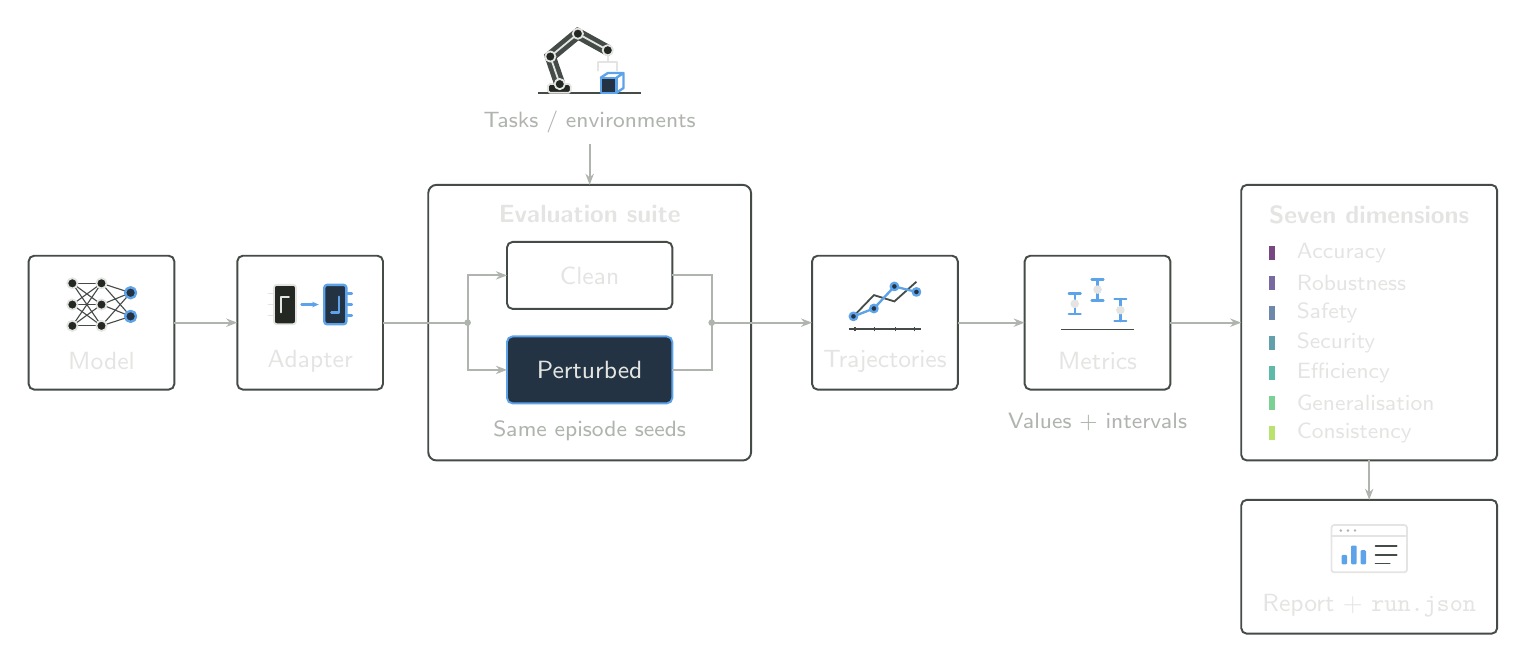
\begin{tikzpicture}[
  x=1cm,y=1cm,
  every node/.style={font=\sffamily\fontsize{9}{11}\selectfont,
    text=ink,inner sep=4pt,outer sep=0pt,align=center},
  box/.style={draw=rule,line width=0.7pt,rounded corners=2pt,
    minimum height=0.85cm,minimum width=1.85cm},
  note/.style={text=muted,font=\sffamily\fontsize{8}{10}\selectfont},
  flow/.style={draw=muted,line width=0.7pt,-{Stealth[length=4pt,width=3pt]}},
  wire/.style={draw=muted,line width=0.7pt},
  icon/.style={draw=ink,line width=0.65pt,line cap=round,line join=round},
  accenticon/.style={draw=signal,line width=0.85pt,line cap=round,line join=round},
  % Small vector illustrations share a two-tone palette and a 0.9 cm footprint.
  pics/model/.style={code={
    \foreach \a in {-0.27,0,0.27} {
      \foreach \b in {-0.27,0,0.27}
        \draw[draw=rule,line width=0.4pt] (-0.37,\a) -- (0,\b);
      \foreach \b in {-0.15,0.15}
        \draw[draw=rule,line width=0.4pt] (0,\a) -- (0.37,\b);
    }
    \foreach \x in {-0.37,0} {
      \foreach \y in {-0.27,0,0.27}
        \draw[icon,fill=panel] (\x,\y) circle (0.065);
    }
    \foreach \y in {-0.15,0.15}
      \draw[accenticon,fill=tint] (0.37,\y) circle (0.07);
  }},
  pics/adapter/.style={code={
    \draw[icon,fill=panel,rounded corners=1pt] (-0.46,-0.25) rectangle (-0.18,0.25);
    \draw[accenticon,fill=tint,rounded corners=1pt] (0.18,-0.25) rectangle (0.46,0.25);
    \foreach \y in {-0.14,0,0.14} {
      \draw[icon] (-0.53,\y) -- (-0.46,\y);
      \draw[accenticon] (0.46,\y) -- (0.53,\y);
    }
    \draw[accenticon,-{Stealth[length=2.4pt,width=2pt]}] (-0.11,0) -- (0.11,0);
    \draw[icon] (-0.37,-0.10) -- (-0.37,0.10) -- (-0.27,0.10);
    \draw[accenticon] (0.27,-0.10) -- (0.37,-0.10) -- (0.37,0.10);
  }},
  pics/trajectory/.style={code={
    \draw[draw=rule,line width=0.45pt] (-0.46,-0.31) -- (0.46,-0.31);
    \foreach \x in {-0.38,-0.13,0.13,0.38}
      \draw[draw=rule,line width=0.45pt] (\x,-0.34) -- (\x,-0.28);
    \draw[draw=rule,line width=0.65pt] (-0.40,-0.15) -- (-0.14,0.12) -- (0.12,0.04) -- (0.40,0.29);
    \draw[accenticon] (-0.40,-0.15) -- (-0.14,-0.05) -- (0.12,0.23) -- (0.40,0.16);
    \foreach \x/\y in {-0.40/-0.15,-0.14/-0.05,0.12/0.23,0.40/0.16}
      \draw[accenticon,fill=tint] (\x,\y) circle (0.047);
  }},
  pics/metrics/.style={code={
    \draw[draw=rule,line width=0.45pt] (-0.46,-0.32) -- (0.46,-0.32);
    \foreach \x/\y/\lo/\hi in {-0.29/0.01/-0.12/0.14,0/0.19/0.05/0.32,0.29/-0.07/-0.21/0.07} {
      \draw[accenticon] (\x,\lo) -- (\x,\hi)
        (\x-0.075,\lo) -- (\x+0.075,\lo)
        (\x-0.075,\hi) -- (\x+0.075,\hi);
      \fill[ink] (\x,\y) circle (0.055);
    }
  }},
  pics/scene/.style={code={
    % Articulated manipulator and an object on its work surface.
    \draw[draw=rule,line width=0.6pt] (-0.65,-0.38) -- (0.65,-0.38);
    \draw[icon,fill=panel,rounded corners=0.7pt] (-0.53,-0.38) rectangle (-0.24,-0.27);
    \draw[draw=rule,line width=4pt,line cap=round] (-0.38,-0.27) -- (-0.50,0.08) -- (-0.15,0.37) -- (0.23,0.16);
    \draw[icon] (-0.38,-0.27) -- (-0.50,0.08) -- (-0.15,0.37) -- (0.23,0.16);
    \foreach \x/\y in {-0.38/-0.27,-0.50/0.08,-0.15/0.37,0.23/0.16}
      \draw[icon,fill=panel] (\x,\y) circle (0.065);
    \draw[icon] (0.23,0.09) -- (0.23,0.01)
      (0.11,-0.10) -- (0.11,0.01) -- (0.35,0.01) -- (0.35,-0.10);
    \draw[accenticon,fill=tint] (0.14,-0.38) rectangle (0.34,-0.19);
    \draw[accenticon] (0.14,-0.19) -- (0.23,-0.13) -- (0.43,-0.13)
      -- (0.34,-0.19) (0.43,-0.13) -- (0.43,-0.32) -- (0.34,-0.38);
  }},
  pics/report/.style={code={
    \draw[icon,rounded corners=1pt] (-0.48,-0.30) rectangle (0.48,0.30);
    \draw[icon] (-0.48,0.16) -- (0.48,0.16);
    \foreach \x in {-0.36,-0.27,-0.18}
      \fill[muted] (\x,0.23) circle (0.018);
    \foreach \x/\h in {-0.35/0.12,-0.23/0.24,-0.11/0.18}
      \fill[signal,rounded corners=0.4pt] (\x,-0.20) rectangle ++(0.07,\h);
    \draw[draw=rule,line width=0.6pt,line cap=round]
      (0.08,0.03) -- (0.35,0.03) (0.08,-0.08) -- (0.35,-0.08)
      (0.08,-0.19) -- (0.26,-0.19);
  }},
]
% The suite branches into matched conditions, whose recorded trajectories feed
% the same metrics. Boxes denote operations or data, never illustrative scores.
\node[box,minimum height=1.70cm] (model) at (0,0) {};
\pic at (0,0.23) {model};
\node at (0,-0.49) {Model};
\node[box,minimum height=1.70cm] (adapter) at (2.65,0) {};
\pic at (2.65,0.23) {adapter};
\node at (2.65,-0.49) {Adapter};
\draw[flow] (model) -- (adapter);

\draw[draw=rule,line width=0.7pt,rounded corners=3pt]
  (4.15,-1.75) rectangle (8.25,1.75);
\node[font=\sffamily\bfseries\fontsize{9}{11}\selectfont]
  at (6.20,1.38) {Evaluation suite};
\node[box,minimum width=2.1cm] (clean) at (6.20,0.60) {Clean};
\node[box,minimum width=2.1cm,draw=signal,fill=tint]
  (perturbed) at (6.20,-0.60) {Perturbed};
\node[note] at (6.20,-1.38) {Same episode seeds};
\coordinate (split) at (4.65,0);
\draw[wire] (adapter.east) -- (split);
\draw[flow] (split) |- (clean.west);
\draw[flow] (split) |- (perturbed.west);
\fill[muted] (split) circle (1.2pt);

\pic at (6.20,3.30) {scene};
\node[note] (tasks) at (6.20,2.55) {Tasks / environments};
\draw[flow] (tasks.south) -- (6.20,1.75);

\node[box,minimum height=1.70cm] (trajectories) at (9.95,0) {};
\pic at (9.95,0.23) {trajectory};
\node at (9.95,-0.49) {Trajectories};
\coordinate (join) at (7.75,0);
\draw[wire] (clean.east) -| (join);
\draw[wire] (perturbed.east) -| (join);
\draw[flow] (join) -- (trajectories.west);
\fill[muted] (join) circle (1.2pt);
\node[box,minimum height=1.70cm] (metrics) at (12.65,0) {};
\pic at (12.65,0.23) {metrics};
\node at (12.65,-0.49) {Metrics};
\draw[flow] (trajectories) -- (metrics);
\node[note,anchor=north] at (12.65,-1.01) {Values + intervals};

% A compact, named output vector avoids fabricating a chart of model scores.
\node[box,minimum width=3.25cm,minimum height=3.50cm]
  (profile) at (16.10,0) {};
\node[font=\sffamily\bfseries\fontsize{9}{11}\selectfont]
  at (16.10,1.37) {Seven dimensions};
\foreach \y/\col/\title in {
  0.88/dimA/Accuracy,
  0.50/dimB/Robustness,
  0.12/dimC/Safety,
  -0.26/dimD/Security,
  -0.64/dimE/Efficiency,
  -1.02/dimF/Generalisation,
  -1.40/dimG/Consistency} {
  \fill[\col] (14.83,\y-0.09) rectangle ++(0.07,0.18);
  \node[anchor=west,font=\sffamily\fontsize{8.5}{10}\selectfont]
    at (15.04,\y) {\title};
}
\draw[flow] (metrics) -- (profile);
\node[box,minimum width=3.25cm,minimum height=1.70cm] (artifacts) at (16.10,-3.10) {};
\pic at (16.10,-2.87) {report};
\node at (16.10,-3.59) {Report + \texttt{run.json}};
\draw[flow] (profile) -- (artifacts);
\end{tikzpicture}
\end{document}
"
%   pdflatex -jobname=method-dark  "\def\xevalstheme{dark}% Documentation method diagram. Build both themes with TeX Live and poppler:
%   pdflatex -jobname=method-light "\def\xevalstheme{light}\input{method.tex}"
%   pdflatex -jobname=method-dark  "\def\xevalstheme{dark}\input{method.tex}"
%   pdftocairo -svg method-light.pdf method-light.svg
%   pdftocairo -svg method-dark.pdf method-dark.svg
% Commit the SVGs; documentation builds do not require LaTeX.
\documentclass[border=8pt]{standalone}
\usepackage[T1]{fontenc}
\usepackage{lmodern}
\usepackage{xcolor}
\usepackage{tikz}
\usetikzlibrary{arrows.meta}
\providecommand{\xevalstheme}{light}
\def\xevalslight{light}
\ifx\xevalstheme\xevalslight
  \definecolor{ink}{HTML}{121412}
  \definecolor{muted}{HTML}{5C615D}
  \definecolor{rule}{HTML}{A8ADA7}
  \definecolor{panel}{HTML}{F1F2EF}
  \definecolor{signal}{HTML}{367FC9}
  \definecolor{tint}{HTML}{E8F0F8}
  \definecolor{dimA}{HTML}{440154}\definecolor{dimB}{HTML}{46327E}
  \definecolor{dimC}{HTML}{365C8D}\definecolor{dimD}{HTML}{277F8E}
  \definecolor{dimE}{HTML}{1FA187}\definecolor{dimF}{HTML}{4AC16D}
  \definecolor{dimG}{HTML}{A0DA39}
\else
  \definecolor{ink}{HTML}{E4E5E2}
  \definecolor{muted}{HTML}{AFB4AE}
  \definecolor{rule}{HTML}{454B46}
  \definecolor{panel}{HTML}{232823}
  \definecolor{signal}{HTML}{5DA3E9}
  \definecolor{tint}{HTML}{233344}
  \definecolor{dimA}{HTML}{774782}\definecolor{dimB}{HTML}{786AA0}
  \definecolor{dimC}{HTML}{6D88AB}\definecolor{dimD}{HTML}{62A1AC}
  \definecolor{dimE}{HTML}{5CBAA7}\definecolor{dimF}{HTML}{7BD194}
  \definecolor{dimG}{HTML}{B9E36E}
\fi
\begin{document}
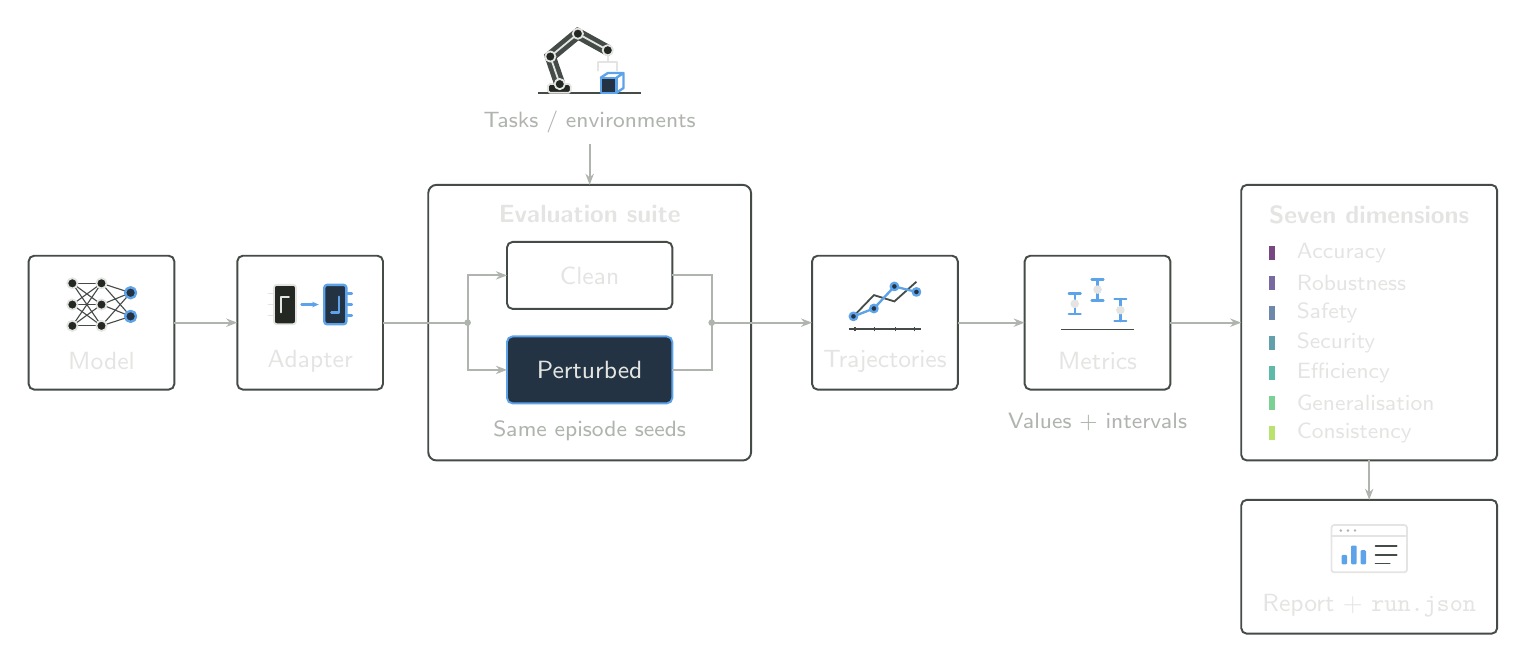
\begin{tikzpicture}[
  x=1cm,y=1cm,
  every node/.style={font=\sffamily\fontsize{9}{11}\selectfont,
    text=ink,inner sep=4pt,outer sep=0pt,align=center},
  box/.style={draw=rule,line width=0.7pt,rounded corners=2pt,
    minimum height=0.85cm,minimum width=1.85cm},
  note/.style={text=muted,font=\sffamily\fontsize{8}{10}\selectfont},
  flow/.style={draw=muted,line width=0.7pt,-{Stealth[length=4pt,width=3pt]}},
  wire/.style={draw=muted,line width=0.7pt},
  icon/.style={draw=ink,line width=0.65pt,line cap=round,line join=round},
  accenticon/.style={draw=signal,line width=0.85pt,line cap=round,line join=round},
  % Small vector illustrations share a two-tone palette and a 0.9 cm footprint.
  pics/model/.style={code={
    \foreach \a in {-0.27,0,0.27} {
      \foreach \b in {-0.27,0,0.27}
        \draw[draw=rule,line width=0.4pt] (-0.37,\a) -- (0,\b);
      \foreach \b in {-0.15,0.15}
        \draw[draw=rule,line width=0.4pt] (0,\a) -- (0.37,\b);
    }
    \foreach \x in {-0.37,0} {
      \foreach \y in {-0.27,0,0.27}
        \draw[icon,fill=panel] (\x,\y) circle (0.065);
    }
    \foreach \y in {-0.15,0.15}
      \draw[accenticon,fill=tint] (0.37,\y) circle (0.07);
  }},
  pics/adapter/.style={code={
    \draw[icon,fill=panel,rounded corners=1pt] (-0.46,-0.25) rectangle (-0.18,0.25);
    \draw[accenticon,fill=tint,rounded corners=1pt] (0.18,-0.25) rectangle (0.46,0.25);
    \foreach \y in {-0.14,0,0.14} {
      \draw[icon] (-0.53,\y) -- (-0.46,\y);
      \draw[accenticon] (0.46,\y) -- (0.53,\y);
    }
    \draw[accenticon,-{Stealth[length=2.4pt,width=2pt]}] (-0.11,0) -- (0.11,0);
    \draw[icon] (-0.37,-0.10) -- (-0.37,0.10) -- (-0.27,0.10);
    \draw[accenticon] (0.27,-0.10) -- (0.37,-0.10) -- (0.37,0.10);
  }},
  pics/trajectory/.style={code={
    \draw[draw=rule,line width=0.45pt] (-0.46,-0.31) -- (0.46,-0.31);
    \foreach \x in {-0.38,-0.13,0.13,0.38}
      \draw[draw=rule,line width=0.45pt] (\x,-0.34) -- (\x,-0.28);
    \draw[draw=rule,line width=0.65pt] (-0.40,-0.15) -- (-0.14,0.12) -- (0.12,0.04) -- (0.40,0.29);
    \draw[accenticon] (-0.40,-0.15) -- (-0.14,-0.05) -- (0.12,0.23) -- (0.40,0.16);
    \foreach \x/\y in {-0.40/-0.15,-0.14/-0.05,0.12/0.23,0.40/0.16}
      \draw[accenticon,fill=tint] (\x,\y) circle (0.047);
  }},
  pics/metrics/.style={code={
    \draw[draw=rule,line width=0.45pt] (-0.46,-0.32) -- (0.46,-0.32);
    \foreach \x/\y/\lo/\hi in {-0.29/0.01/-0.12/0.14,0/0.19/0.05/0.32,0.29/-0.07/-0.21/0.07} {
      \draw[accenticon] (\x,\lo) -- (\x,\hi)
        (\x-0.075,\lo) -- (\x+0.075,\lo)
        (\x-0.075,\hi) -- (\x+0.075,\hi);
      \fill[ink] (\x,\y) circle (0.055);
    }
  }},
  pics/scene/.style={code={
    % Articulated manipulator and an object on its work surface.
    \draw[draw=rule,line width=0.6pt] (-0.65,-0.38) -- (0.65,-0.38);
    \draw[icon,fill=panel,rounded corners=0.7pt] (-0.53,-0.38) rectangle (-0.24,-0.27);
    \draw[draw=rule,line width=4pt,line cap=round] (-0.38,-0.27) -- (-0.50,0.08) -- (-0.15,0.37) -- (0.23,0.16);
    \draw[icon] (-0.38,-0.27) -- (-0.50,0.08) -- (-0.15,0.37) -- (0.23,0.16);
    \foreach \x/\y in {-0.38/-0.27,-0.50/0.08,-0.15/0.37,0.23/0.16}
      \draw[icon,fill=panel] (\x,\y) circle (0.065);
    \draw[icon] (0.23,0.09) -- (0.23,0.01)
      (0.11,-0.10) -- (0.11,0.01) -- (0.35,0.01) -- (0.35,-0.10);
    \draw[accenticon,fill=tint] (0.14,-0.38) rectangle (0.34,-0.19);
    \draw[accenticon] (0.14,-0.19) -- (0.23,-0.13) -- (0.43,-0.13)
      -- (0.34,-0.19) (0.43,-0.13) -- (0.43,-0.32) -- (0.34,-0.38);
  }},
  pics/report/.style={code={
    \draw[icon,rounded corners=1pt] (-0.48,-0.30) rectangle (0.48,0.30);
    \draw[icon] (-0.48,0.16) -- (0.48,0.16);
    \foreach \x in {-0.36,-0.27,-0.18}
      \fill[muted] (\x,0.23) circle (0.018);
    \foreach \x/\h in {-0.35/0.12,-0.23/0.24,-0.11/0.18}
      \fill[signal,rounded corners=0.4pt] (\x,-0.20) rectangle ++(0.07,\h);
    \draw[draw=rule,line width=0.6pt,line cap=round]
      (0.08,0.03) -- (0.35,0.03) (0.08,-0.08) -- (0.35,-0.08)
      (0.08,-0.19) -- (0.26,-0.19);
  }},
]
% The suite branches into matched conditions, whose recorded trajectories feed
% the same metrics. Boxes denote operations or data, never illustrative scores.
\node[box,minimum height=1.70cm] (model) at (0,0) {};
\pic at (0,0.23) {model};
\node at (0,-0.49) {Model};
\node[box,minimum height=1.70cm] (adapter) at (2.65,0) {};
\pic at (2.65,0.23) {adapter};
\node at (2.65,-0.49) {Adapter};
\draw[flow] (model) -- (adapter);

\draw[draw=rule,line width=0.7pt,rounded corners=3pt]
  (4.15,-1.75) rectangle (8.25,1.75);
\node[font=\sffamily\bfseries\fontsize{9}{11}\selectfont]
  at (6.20,1.38) {Evaluation suite};
\node[box,minimum width=2.1cm] (clean) at (6.20,0.60) {Clean};
\node[box,minimum width=2.1cm,draw=signal,fill=tint]
  (perturbed) at (6.20,-0.60) {Perturbed};
\node[note] at (6.20,-1.38) {Same episode seeds};
\coordinate (split) at (4.65,0);
\draw[wire] (adapter.east) -- (split);
\draw[flow] (split) |- (clean.west);
\draw[flow] (split) |- (perturbed.west);
\fill[muted] (split) circle (1.2pt);

\pic at (6.20,3.30) {scene};
\node[note] (tasks) at (6.20,2.55) {Tasks / environments};
\draw[flow] (tasks.south) -- (6.20,1.75);

\node[box,minimum height=1.70cm] (trajectories) at (9.95,0) {};
\pic at (9.95,0.23) {trajectory};
\node at (9.95,-0.49) {Trajectories};
\coordinate (join) at (7.75,0);
\draw[wire] (clean.east) -| (join);
\draw[wire] (perturbed.east) -| (join);
\draw[flow] (join) -- (trajectories.west);
\fill[muted] (join) circle (1.2pt);
\node[box,minimum height=1.70cm] (metrics) at (12.65,0) {};
\pic at (12.65,0.23) {metrics};
\node at (12.65,-0.49) {Metrics};
\draw[flow] (trajectories) -- (metrics);
\node[note,anchor=north] at (12.65,-1.01) {Values + intervals};

% A compact, named output vector avoids fabricating a chart of model scores.
\node[box,minimum width=3.25cm,minimum height=3.50cm]
  (profile) at (16.10,0) {};
\node[font=\sffamily\bfseries\fontsize{9}{11}\selectfont]
  at (16.10,1.37) {Seven dimensions};
\foreach \y/\col/\title in {
  0.88/dimA/Accuracy,
  0.50/dimB/Robustness,
  0.12/dimC/Safety,
  -0.26/dimD/Security,
  -0.64/dimE/Efficiency,
  -1.02/dimF/Generalisation,
  -1.40/dimG/Consistency} {
  \fill[\col] (14.83,\y-0.09) rectangle ++(0.07,0.18);
  \node[anchor=west,font=\sffamily\fontsize{8.5}{10}\selectfont]
    at (15.04,\y) {\title};
}
\draw[flow] (metrics) -- (profile);
\node[box,minimum width=3.25cm,minimum height=1.70cm] (artifacts) at (16.10,-3.10) {};
\pic at (16.10,-2.87) {report};
\node at (16.10,-3.59) {Report + \texttt{run.json}};
\draw[flow] (profile) -- (artifacts);
\end{tikzpicture}
\end{document}
"
%   pdftocairo -svg method-light.pdf method-light.svg
%   pdftocairo -svg method-dark.pdf method-dark.svg
% Commit the SVGs; documentation builds do not require LaTeX.
\documentclass[border=8pt]{standalone}
\usepackage[T1]{fontenc}
\usepackage{lmodern}
\usepackage{xcolor}
\usepackage{tikz}
\usetikzlibrary{arrows.meta}
\providecommand{\xevalstheme}{light}
\def\xevalslight{light}
\ifx\xevalstheme\xevalslight
  \definecolor{ink}{HTML}{121412}
  \definecolor{muted}{HTML}{5C615D}
  \definecolor{rule}{HTML}{A8ADA7}
  \definecolor{panel}{HTML}{F1F2EF}
  \definecolor{signal}{HTML}{367FC9}
  \definecolor{tint}{HTML}{E8F0F8}
  \definecolor{dimA}{HTML}{440154}\definecolor{dimB}{HTML}{46327E}
  \definecolor{dimC}{HTML}{365C8D}\definecolor{dimD}{HTML}{277F8E}
  \definecolor{dimE}{HTML}{1FA187}\definecolor{dimF}{HTML}{4AC16D}
  \definecolor{dimG}{HTML}{A0DA39}
\else
  \definecolor{ink}{HTML}{E4E5E2}
  \definecolor{muted}{HTML}{AFB4AE}
  \definecolor{rule}{HTML}{454B46}
  \definecolor{panel}{HTML}{232823}
  \definecolor{signal}{HTML}{5DA3E9}
  \definecolor{tint}{HTML}{233344}
  \definecolor{dimA}{HTML}{774782}\definecolor{dimB}{HTML}{786AA0}
  \definecolor{dimC}{HTML}{6D88AB}\definecolor{dimD}{HTML}{62A1AC}
  \definecolor{dimE}{HTML}{5CBAA7}\definecolor{dimF}{HTML}{7BD194}
  \definecolor{dimG}{HTML}{B9E36E}
\fi
\begin{document}
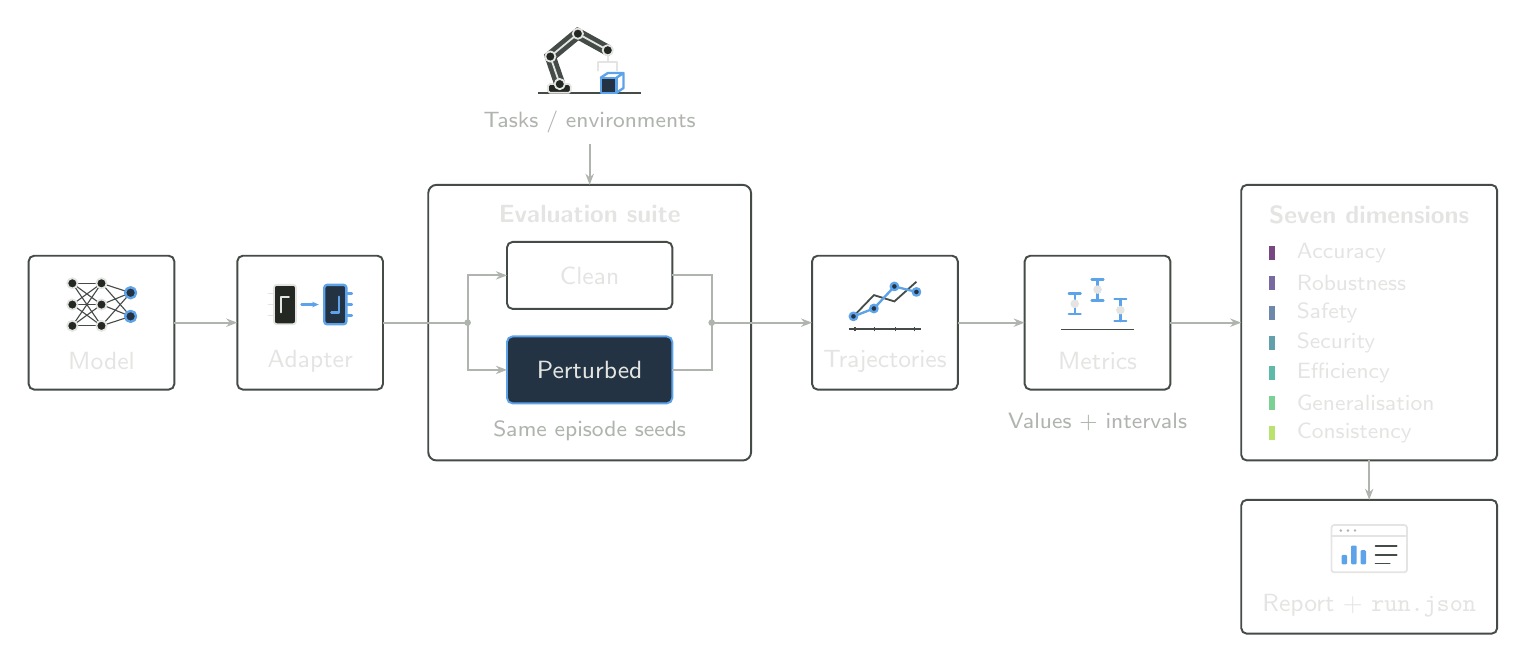
\begin{tikzpicture}[
  x=1cm,y=1cm,
  every node/.style={font=\sffamily\fontsize{9}{11}\selectfont,
    text=ink,inner sep=4pt,outer sep=0pt,align=center},
  box/.style={draw=rule,line width=0.7pt,rounded corners=2pt,
    minimum height=0.85cm,minimum width=1.85cm},
  note/.style={text=muted,font=\sffamily\fontsize{8}{10}\selectfont},
  flow/.style={draw=muted,line width=0.7pt,-{Stealth[length=4pt,width=3pt]}},
  wire/.style={draw=muted,line width=0.7pt},
  icon/.style={draw=ink,line width=0.65pt,line cap=round,line join=round},
  accenticon/.style={draw=signal,line width=0.85pt,line cap=round,line join=round},
  % Small vector illustrations share a two-tone palette and a 0.9 cm footprint.
  pics/model/.style={code={
    \foreach \a in {-0.27,0,0.27} {
      \foreach \b in {-0.27,0,0.27}
        \draw[draw=rule,line width=0.4pt] (-0.37,\a) -- (0,\b);
      \foreach \b in {-0.15,0.15}
        \draw[draw=rule,line width=0.4pt] (0,\a) -- (0.37,\b);
    }
    \foreach \x in {-0.37,0} {
      \foreach \y in {-0.27,0,0.27}
        \draw[icon,fill=panel] (\x,\y) circle (0.065);
    }
    \foreach \y in {-0.15,0.15}
      \draw[accenticon,fill=tint] (0.37,\y) circle (0.07);
  }},
  pics/adapter/.style={code={
    \draw[icon,fill=panel,rounded corners=1pt] (-0.46,-0.25) rectangle (-0.18,0.25);
    \draw[accenticon,fill=tint,rounded corners=1pt] (0.18,-0.25) rectangle (0.46,0.25);
    \foreach \y in {-0.14,0,0.14} {
      \draw[icon] (-0.53,\y) -- (-0.46,\y);
      \draw[accenticon] (0.46,\y) -- (0.53,\y);
    }
    \draw[accenticon,-{Stealth[length=2.4pt,width=2pt]}] (-0.11,0) -- (0.11,0);
    \draw[icon] (-0.37,-0.10) -- (-0.37,0.10) -- (-0.27,0.10);
    \draw[accenticon] (0.27,-0.10) -- (0.37,-0.10) -- (0.37,0.10);
  }},
  pics/trajectory/.style={code={
    \draw[draw=rule,line width=0.45pt] (-0.46,-0.31) -- (0.46,-0.31);
    \foreach \x in {-0.38,-0.13,0.13,0.38}
      \draw[draw=rule,line width=0.45pt] (\x,-0.34) -- (\x,-0.28);
    \draw[draw=rule,line width=0.65pt] (-0.40,-0.15) -- (-0.14,0.12) -- (0.12,0.04) -- (0.40,0.29);
    \draw[accenticon] (-0.40,-0.15) -- (-0.14,-0.05) -- (0.12,0.23) -- (0.40,0.16);
    \foreach \x/\y in {-0.40/-0.15,-0.14/-0.05,0.12/0.23,0.40/0.16}
      \draw[accenticon,fill=tint] (\x,\y) circle (0.047);
  }},
  pics/metrics/.style={code={
    \draw[draw=rule,line width=0.45pt] (-0.46,-0.32) -- (0.46,-0.32);
    \foreach \x/\y/\lo/\hi in {-0.29/0.01/-0.12/0.14,0/0.19/0.05/0.32,0.29/-0.07/-0.21/0.07} {
      \draw[accenticon] (\x,\lo) -- (\x,\hi)
        (\x-0.075,\lo) -- (\x+0.075,\lo)
        (\x-0.075,\hi) -- (\x+0.075,\hi);
      \fill[ink] (\x,\y) circle (0.055);
    }
  }},
  pics/scene/.style={code={
    % Articulated manipulator and an object on its work surface.
    \draw[draw=rule,line width=0.6pt] (-0.65,-0.38) -- (0.65,-0.38);
    \draw[icon,fill=panel,rounded corners=0.7pt] (-0.53,-0.38) rectangle (-0.24,-0.27);
    \draw[draw=rule,line width=4pt,line cap=round] (-0.38,-0.27) -- (-0.50,0.08) -- (-0.15,0.37) -- (0.23,0.16);
    \draw[icon] (-0.38,-0.27) -- (-0.50,0.08) -- (-0.15,0.37) -- (0.23,0.16);
    \foreach \x/\y in {-0.38/-0.27,-0.50/0.08,-0.15/0.37,0.23/0.16}
      \draw[icon,fill=panel] (\x,\y) circle (0.065);
    \draw[icon] (0.23,0.09) -- (0.23,0.01)
      (0.11,-0.10) -- (0.11,0.01) -- (0.35,0.01) -- (0.35,-0.10);
    \draw[accenticon,fill=tint] (0.14,-0.38) rectangle (0.34,-0.19);
    \draw[accenticon] (0.14,-0.19) -- (0.23,-0.13) -- (0.43,-0.13)
      -- (0.34,-0.19) (0.43,-0.13) -- (0.43,-0.32) -- (0.34,-0.38);
  }},
  pics/report/.style={code={
    \draw[icon,rounded corners=1pt] (-0.48,-0.30) rectangle (0.48,0.30);
    \draw[icon] (-0.48,0.16) -- (0.48,0.16);
    \foreach \x in {-0.36,-0.27,-0.18}
      \fill[muted] (\x,0.23) circle (0.018);
    \foreach \x/\h in {-0.35/0.12,-0.23/0.24,-0.11/0.18}
      \fill[signal,rounded corners=0.4pt] (\x,-0.20) rectangle ++(0.07,\h);
    \draw[draw=rule,line width=0.6pt,line cap=round]
      (0.08,0.03) -- (0.35,0.03) (0.08,-0.08) -- (0.35,-0.08)
      (0.08,-0.19) -- (0.26,-0.19);
  }},
]
% The suite branches into matched conditions, whose recorded trajectories feed
% the same metrics. Boxes denote operations or data, never illustrative scores.
\node[box,minimum height=1.70cm] (model) at (0,0) {};
\pic at (0,0.23) {model};
\node at (0,-0.49) {Model};
\node[box,minimum height=1.70cm] (adapter) at (2.65,0) {};
\pic at (2.65,0.23) {adapter};
\node at (2.65,-0.49) {Adapter};
\draw[flow] (model) -- (adapter);

\draw[draw=rule,line width=0.7pt,rounded corners=3pt]
  (4.15,-1.75) rectangle (8.25,1.75);
\node[font=\sffamily\bfseries\fontsize{9}{11}\selectfont]
  at (6.20,1.38) {Evaluation suite};
\node[box,minimum width=2.1cm] (clean) at (6.20,0.60) {Clean};
\node[box,minimum width=2.1cm,draw=signal,fill=tint]
  (perturbed) at (6.20,-0.60) {Perturbed};
\node[note] at (6.20,-1.38) {Same episode seeds};
\coordinate (split) at (4.65,0);
\draw[wire] (adapter.east) -- (split);
\draw[flow] (split) |- (clean.west);
\draw[flow] (split) |- (perturbed.west);
\fill[muted] (split) circle (1.2pt);

\pic at (6.20,3.30) {scene};
\node[note] (tasks) at (6.20,2.55) {Tasks / environments};
\draw[flow] (tasks.south) -- (6.20,1.75);

\node[box,minimum height=1.70cm] (trajectories) at (9.95,0) {};
\pic at (9.95,0.23) {trajectory};
\node at (9.95,-0.49) {Trajectories};
\coordinate (join) at (7.75,0);
\draw[wire] (clean.east) -| (join);
\draw[wire] (perturbed.east) -| (join);
\draw[flow] (join) -- (trajectories.west);
\fill[muted] (join) circle (1.2pt);
\node[box,minimum height=1.70cm] (metrics) at (12.65,0) {};
\pic at (12.65,0.23) {metrics};
\node at (12.65,-0.49) {Metrics};
\draw[flow] (trajectories) -- (metrics);
\node[note,anchor=north] at (12.65,-1.01) {Values + intervals};

% A compact, named output vector avoids fabricating a chart of model scores.
\node[box,minimum width=3.25cm,minimum height=3.50cm]
  (profile) at (16.10,0) {};
\node[font=\sffamily\bfseries\fontsize{9}{11}\selectfont]
  at (16.10,1.37) {Seven dimensions};
\foreach \y/\col/\title in {
  0.88/dimA/Accuracy,
  0.50/dimB/Robustness,
  0.12/dimC/Safety,
  -0.26/dimD/Security,
  -0.64/dimE/Efficiency,
  -1.02/dimF/Generalisation,
  -1.40/dimG/Consistency} {
  \fill[\col] (14.83,\y-0.09) rectangle ++(0.07,0.18);
  \node[anchor=west,font=\sffamily\fontsize{8.5}{10}\selectfont]
    at (15.04,\y) {\title};
}
\draw[flow] (metrics) -- (profile);
\node[box,minimum width=3.25cm,minimum height=1.70cm] (artifacts) at (16.10,-3.10) {};
\pic at (16.10,-2.87) {report};
\node at (16.10,-3.59) {Report + \texttt{run.json}};
\draw[flow] (profile) -- (artifacts);
\end{tikzpicture}
\end{document}
"
%   pdflatex -jobname=method-dark  "\def\xevalstheme{dark}% Documentation method diagram. Build both themes with TeX Live and poppler:
%   pdflatex -jobname=method-light "\def\xevalstheme{light}% Documentation method diagram. Build both themes with TeX Live and poppler:
%   pdflatex -jobname=method-light "\def\xevalstheme{light}\input{method.tex}"
%   pdflatex -jobname=method-dark  "\def\xevalstheme{dark}\input{method.tex}"
%   pdftocairo -svg method-light.pdf method-light.svg
%   pdftocairo -svg method-dark.pdf method-dark.svg
% Commit the SVGs; documentation builds do not require LaTeX.
\documentclass[border=8pt]{standalone}
\usepackage[T1]{fontenc}
\usepackage{lmodern}
\usepackage{xcolor}
\usepackage{tikz}
\usetikzlibrary{arrows.meta}
\providecommand{\xevalstheme}{light}
\def\xevalslight{light}
\ifx\xevalstheme\xevalslight
  \definecolor{ink}{HTML}{121412}
  \definecolor{muted}{HTML}{5C615D}
  \definecolor{rule}{HTML}{A8ADA7}
  \definecolor{panel}{HTML}{F1F2EF}
  \definecolor{signal}{HTML}{367FC9}
  \definecolor{tint}{HTML}{E8F0F8}
  \definecolor{dimA}{HTML}{440154}\definecolor{dimB}{HTML}{46327E}
  \definecolor{dimC}{HTML}{365C8D}\definecolor{dimD}{HTML}{277F8E}
  \definecolor{dimE}{HTML}{1FA187}\definecolor{dimF}{HTML}{4AC16D}
  \definecolor{dimG}{HTML}{A0DA39}
\else
  \definecolor{ink}{HTML}{E4E5E2}
  \definecolor{muted}{HTML}{AFB4AE}
  \definecolor{rule}{HTML}{454B46}
  \definecolor{panel}{HTML}{232823}
  \definecolor{signal}{HTML}{5DA3E9}
  \definecolor{tint}{HTML}{233344}
  \definecolor{dimA}{HTML}{774782}\definecolor{dimB}{HTML}{786AA0}
  \definecolor{dimC}{HTML}{6D88AB}\definecolor{dimD}{HTML}{62A1AC}
  \definecolor{dimE}{HTML}{5CBAA7}\definecolor{dimF}{HTML}{7BD194}
  \definecolor{dimG}{HTML}{B9E36E}
\fi
\begin{document}
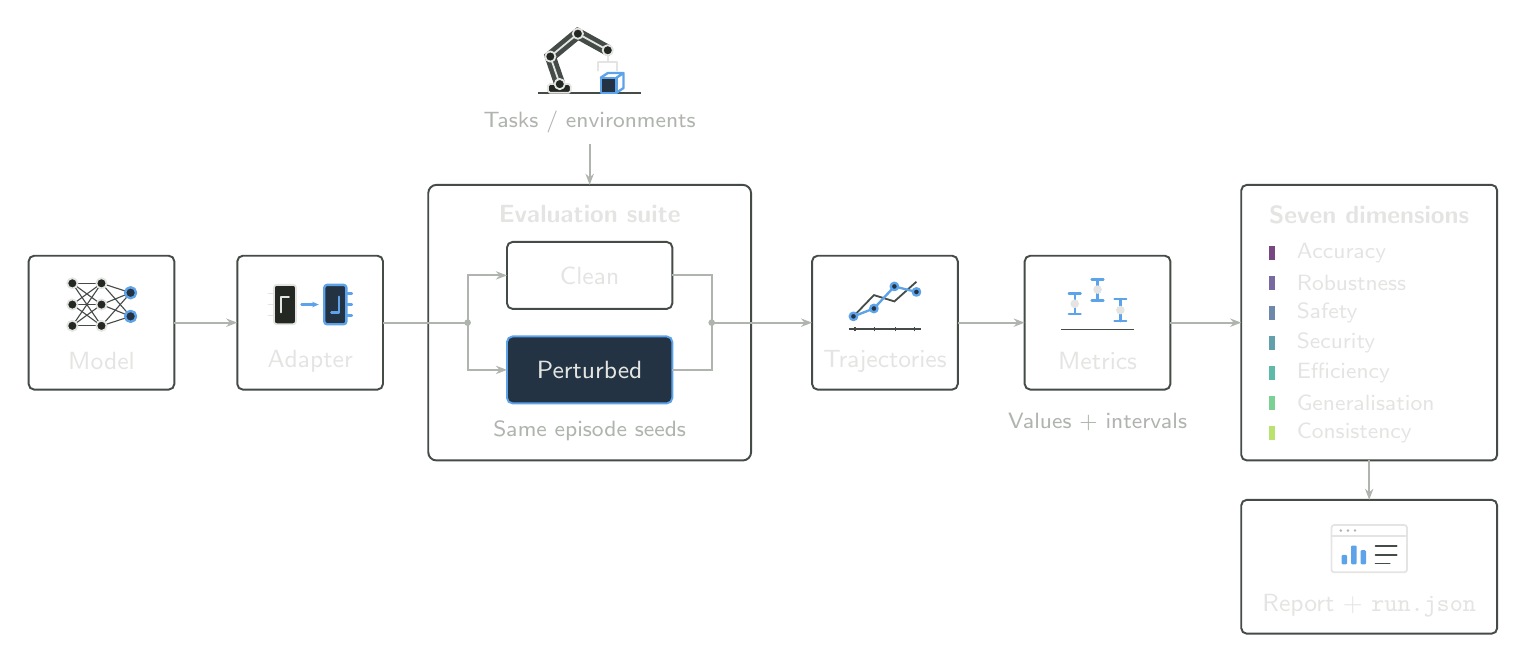
\begin{tikzpicture}[
  x=1cm,y=1cm,
  every node/.style={font=\sffamily\fontsize{9}{11}\selectfont,
    text=ink,inner sep=4pt,outer sep=0pt,align=center},
  box/.style={draw=rule,line width=0.7pt,rounded corners=2pt,
    minimum height=0.85cm,minimum width=1.85cm},
  note/.style={text=muted,font=\sffamily\fontsize{8}{10}\selectfont},
  flow/.style={draw=muted,line width=0.7pt,-{Stealth[length=4pt,width=3pt]}},
  wire/.style={draw=muted,line width=0.7pt},
  icon/.style={draw=ink,line width=0.65pt,line cap=round,line join=round},
  accenticon/.style={draw=signal,line width=0.85pt,line cap=round,line join=round},
  % Small vector illustrations share a two-tone palette and a 0.9 cm footprint.
  pics/model/.style={code={
    \foreach \a in {-0.27,0,0.27} {
      \foreach \b in {-0.27,0,0.27}
        \draw[draw=rule,line width=0.4pt] (-0.37,\a) -- (0,\b);
      \foreach \b in {-0.15,0.15}
        \draw[draw=rule,line width=0.4pt] (0,\a) -- (0.37,\b);
    }
    \foreach \x in {-0.37,0} {
      \foreach \y in {-0.27,0,0.27}
        \draw[icon,fill=panel] (\x,\y) circle (0.065);
    }
    \foreach \y in {-0.15,0.15}
      \draw[accenticon,fill=tint] (0.37,\y) circle (0.07);
  }},
  pics/adapter/.style={code={
    \draw[icon,fill=panel,rounded corners=1pt] (-0.46,-0.25) rectangle (-0.18,0.25);
    \draw[accenticon,fill=tint,rounded corners=1pt] (0.18,-0.25) rectangle (0.46,0.25);
    \foreach \y in {-0.14,0,0.14} {
      \draw[icon] (-0.53,\y) -- (-0.46,\y);
      \draw[accenticon] (0.46,\y) -- (0.53,\y);
    }
    \draw[accenticon,-{Stealth[length=2.4pt,width=2pt]}] (-0.11,0) -- (0.11,0);
    \draw[icon] (-0.37,-0.10) -- (-0.37,0.10) -- (-0.27,0.10);
    \draw[accenticon] (0.27,-0.10) -- (0.37,-0.10) -- (0.37,0.10);
  }},
  pics/trajectory/.style={code={
    \draw[draw=rule,line width=0.45pt] (-0.46,-0.31) -- (0.46,-0.31);
    \foreach \x in {-0.38,-0.13,0.13,0.38}
      \draw[draw=rule,line width=0.45pt] (\x,-0.34) -- (\x,-0.28);
    \draw[draw=rule,line width=0.65pt] (-0.40,-0.15) -- (-0.14,0.12) -- (0.12,0.04) -- (0.40,0.29);
    \draw[accenticon] (-0.40,-0.15) -- (-0.14,-0.05) -- (0.12,0.23) -- (0.40,0.16);
    \foreach \x/\y in {-0.40/-0.15,-0.14/-0.05,0.12/0.23,0.40/0.16}
      \draw[accenticon,fill=tint] (\x,\y) circle (0.047);
  }},
  pics/metrics/.style={code={
    \draw[draw=rule,line width=0.45pt] (-0.46,-0.32) -- (0.46,-0.32);
    \foreach \x/\y/\lo/\hi in {-0.29/0.01/-0.12/0.14,0/0.19/0.05/0.32,0.29/-0.07/-0.21/0.07} {
      \draw[accenticon] (\x,\lo) -- (\x,\hi)
        (\x-0.075,\lo) -- (\x+0.075,\lo)
        (\x-0.075,\hi) -- (\x+0.075,\hi);
      \fill[ink] (\x,\y) circle (0.055);
    }
  }},
  pics/scene/.style={code={
    % Articulated manipulator and an object on its work surface.
    \draw[draw=rule,line width=0.6pt] (-0.65,-0.38) -- (0.65,-0.38);
    \draw[icon,fill=panel,rounded corners=0.7pt] (-0.53,-0.38) rectangle (-0.24,-0.27);
    \draw[draw=rule,line width=4pt,line cap=round] (-0.38,-0.27) -- (-0.50,0.08) -- (-0.15,0.37) -- (0.23,0.16);
    \draw[icon] (-0.38,-0.27) -- (-0.50,0.08) -- (-0.15,0.37) -- (0.23,0.16);
    \foreach \x/\y in {-0.38/-0.27,-0.50/0.08,-0.15/0.37,0.23/0.16}
      \draw[icon,fill=panel] (\x,\y) circle (0.065);
    \draw[icon] (0.23,0.09) -- (0.23,0.01)
      (0.11,-0.10) -- (0.11,0.01) -- (0.35,0.01) -- (0.35,-0.10);
    \draw[accenticon,fill=tint] (0.14,-0.38) rectangle (0.34,-0.19);
    \draw[accenticon] (0.14,-0.19) -- (0.23,-0.13) -- (0.43,-0.13)
      -- (0.34,-0.19) (0.43,-0.13) -- (0.43,-0.32) -- (0.34,-0.38);
  }},
  pics/report/.style={code={
    \draw[icon,rounded corners=1pt] (-0.48,-0.30) rectangle (0.48,0.30);
    \draw[icon] (-0.48,0.16) -- (0.48,0.16);
    \foreach \x in {-0.36,-0.27,-0.18}
      \fill[muted] (\x,0.23) circle (0.018);
    \foreach \x/\h in {-0.35/0.12,-0.23/0.24,-0.11/0.18}
      \fill[signal,rounded corners=0.4pt] (\x,-0.20) rectangle ++(0.07,\h);
    \draw[draw=rule,line width=0.6pt,line cap=round]
      (0.08,0.03) -- (0.35,0.03) (0.08,-0.08) -- (0.35,-0.08)
      (0.08,-0.19) -- (0.26,-0.19);
  }},
]
% The suite branches into matched conditions, whose recorded trajectories feed
% the same metrics. Boxes denote operations or data, never illustrative scores.
\node[box,minimum height=1.70cm] (model) at (0,0) {};
\pic at (0,0.23) {model};
\node at (0,-0.49) {Model};
\node[box,minimum height=1.70cm] (adapter) at (2.65,0) {};
\pic at (2.65,0.23) {adapter};
\node at (2.65,-0.49) {Adapter};
\draw[flow] (model) -- (adapter);

\draw[draw=rule,line width=0.7pt,rounded corners=3pt]
  (4.15,-1.75) rectangle (8.25,1.75);
\node[font=\sffamily\bfseries\fontsize{9}{11}\selectfont]
  at (6.20,1.38) {Evaluation suite};
\node[box,minimum width=2.1cm] (clean) at (6.20,0.60) {Clean};
\node[box,minimum width=2.1cm,draw=signal,fill=tint]
  (perturbed) at (6.20,-0.60) {Perturbed};
\node[note] at (6.20,-1.38) {Same episode seeds};
\coordinate (split) at (4.65,0);
\draw[wire] (adapter.east) -- (split);
\draw[flow] (split) |- (clean.west);
\draw[flow] (split) |- (perturbed.west);
\fill[muted] (split) circle (1.2pt);

\pic at (6.20,3.30) {scene};
\node[note] (tasks) at (6.20,2.55) {Tasks / environments};
\draw[flow] (tasks.south) -- (6.20,1.75);

\node[box,minimum height=1.70cm] (trajectories) at (9.95,0) {};
\pic at (9.95,0.23) {trajectory};
\node at (9.95,-0.49) {Trajectories};
\coordinate (join) at (7.75,0);
\draw[wire] (clean.east) -| (join);
\draw[wire] (perturbed.east) -| (join);
\draw[flow] (join) -- (trajectories.west);
\fill[muted] (join) circle (1.2pt);
\node[box,minimum height=1.70cm] (metrics) at (12.65,0) {};
\pic at (12.65,0.23) {metrics};
\node at (12.65,-0.49) {Metrics};
\draw[flow] (trajectories) -- (metrics);
\node[note,anchor=north] at (12.65,-1.01) {Values + intervals};

% A compact, named output vector avoids fabricating a chart of model scores.
\node[box,minimum width=3.25cm,minimum height=3.50cm]
  (profile) at (16.10,0) {};
\node[font=\sffamily\bfseries\fontsize{9}{11}\selectfont]
  at (16.10,1.37) {Seven dimensions};
\foreach \y/\col/\title in {
  0.88/dimA/Accuracy,
  0.50/dimB/Robustness,
  0.12/dimC/Safety,
  -0.26/dimD/Security,
  -0.64/dimE/Efficiency,
  -1.02/dimF/Generalisation,
  -1.40/dimG/Consistency} {
  \fill[\col] (14.83,\y-0.09) rectangle ++(0.07,0.18);
  \node[anchor=west,font=\sffamily\fontsize{8.5}{10}\selectfont]
    at (15.04,\y) {\title};
}
\draw[flow] (metrics) -- (profile);
\node[box,minimum width=3.25cm,minimum height=1.70cm] (artifacts) at (16.10,-3.10) {};
\pic at (16.10,-2.87) {report};
\node at (16.10,-3.59) {Report + \texttt{run.json}};
\draw[flow] (profile) -- (artifacts);
\end{tikzpicture}
\end{document}
"
%   pdflatex -jobname=method-dark  "\def\xevalstheme{dark}% Documentation method diagram. Build both themes with TeX Live and poppler:
%   pdflatex -jobname=method-light "\def\xevalstheme{light}\input{method.tex}"
%   pdflatex -jobname=method-dark  "\def\xevalstheme{dark}\input{method.tex}"
%   pdftocairo -svg method-light.pdf method-light.svg
%   pdftocairo -svg method-dark.pdf method-dark.svg
% Commit the SVGs; documentation builds do not require LaTeX.
\documentclass[border=8pt]{standalone}
\usepackage[T1]{fontenc}
\usepackage{lmodern}
\usepackage{xcolor}
\usepackage{tikz}
\usetikzlibrary{arrows.meta}
\providecommand{\xevalstheme}{light}
\def\xevalslight{light}
\ifx\xevalstheme\xevalslight
  \definecolor{ink}{HTML}{121412}
  \definecolor{muted}{HTML}{5C615D}
  \definecolor{rule}{HTML}{A8ADA7}
  \definecolor{panel}{HTML}{F1F2EF}
  \definecolor{signal}{HTML}{367FC9}
  \definecolor{tint}{HTML}{E8F0F8}
  \definecolor{dimA}{HTML}{440154}\definecolor{dimB}{HTML}{46327E}
  \definecolor{dimC}{HTML}{365C8D}\definecolor{dimD}{HTML}{277F8E}
  \definecolor{dimE}{HTML}{1FA187}\definecolor{dimF}{HTML}{4AC16D}
  \definecolor{dimG}{HTML}{A0DA39}
\else
  \definecolor{ink}{HTML}{E4E5E2}
  \definecolor{muted}{HTML}{AFB4AE}
  \definecolor{rule}{HTML}{454B46}
  \definecolor{panel}{HTML}{232823}
  \definecolor{signal}{HTML}{5DA3E9}
  \definecolor{tint}{HTML}{233344}
  \definecolor{dimA}{HTML}{774782}\definecolor{dimB}{HTML}{786AA0}
  \definecolor{dimC}{HTML}{6D88AB}\definecolor{dimD}{HTML}{62A1AC}
  \definecolor{dimE}{HTML}{5CBAA7}\definecolor{dimF}{HTML}{7BD194}
  \definecolor{dimG}{HTML}{B9E36E}
\fi
\begin{document}
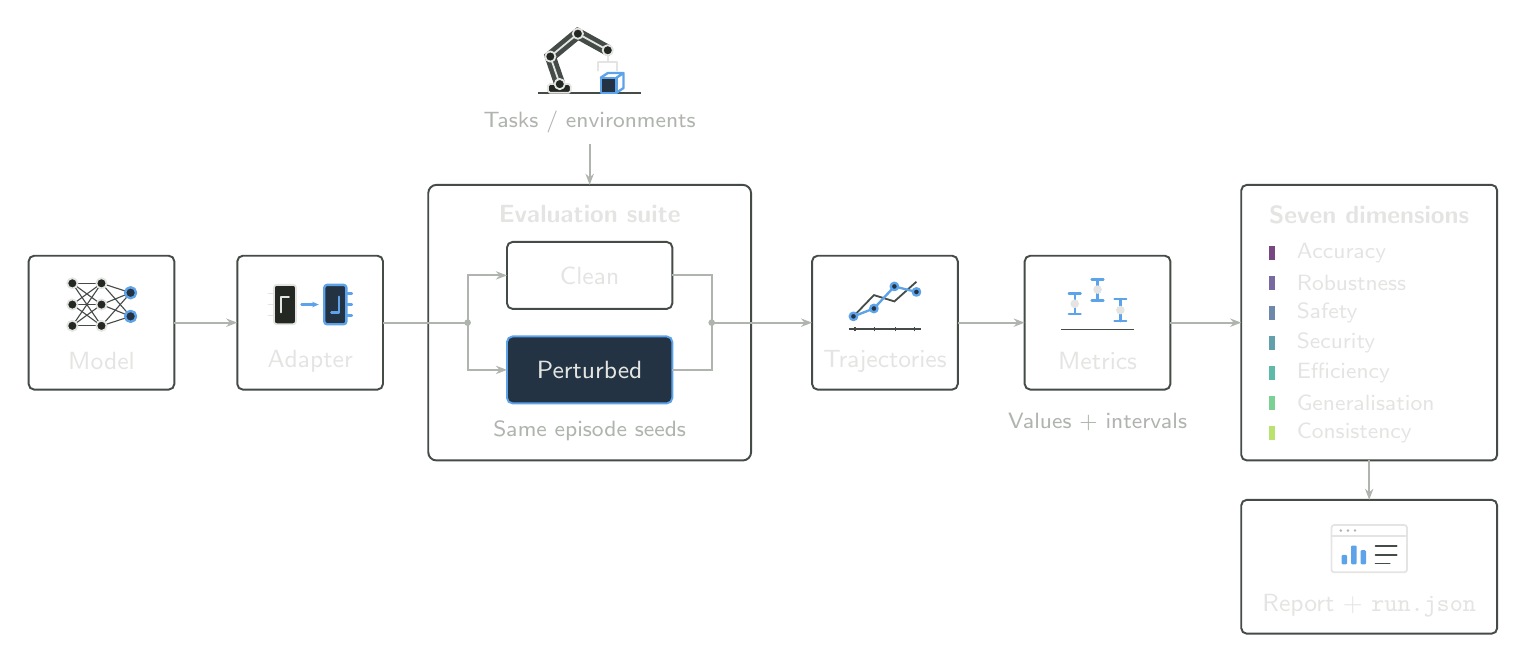
\begin{tikzpicture}[
  x=1cm,y=1cm,
  every node/.style={font=\sffamily\fontsize{9}{11}\selectfont,
    text=ink,inner sep=4pt,outer sep=0pt,align=center},
  box/.style={draw=rule,line width=0.7pt,rounded corners=2pt,
    minimum height=0.85cm,minimum width=1.85cm},
  note/.style={text=muted,font=\sffamily\fontsize{8}{10}\selectfont},
  flow/.style={draw=muted,line width=0.7pt,-{Stealth[length=4pt,width=3pt]}},
  wire/.style={draw=muted,line width=0.7pt},
  icon/.style={draw=ink,line width=0.65pt,line cap=round,line join=round},
  accenticon/.style={draw=signal,line width=0.85pt,line cap=round,line join=round},
  % Small vector illustrations share a two-tone palette and a 0.9 cm footprint.
  pics/model/.style={code={
    \foreach \a in {-0.27,0,0.27} {
      \foreach \b in {-0.27,0,0.27}
        \draw[draw=rule,line width=0.4pt] (-0.37,\a) -- (0,\b);
      \foreach \b in {-0.15,0.15}
        \draw[draw=rule,line width=0.4pt] (0,\a) -- (0.37,\b);
    }
    \foreach \x in {-0.37,0} {
      \foreach \y in {-0.27,0,0.27}
        \draw[icon,fill=panel] (\x,\y) circle (0.065);
    }
    \foreach \y in {-0.15,0.15}
      \draw[accenticon,fill=tint] (0.37,\y) circle (0.07);
  }},
  pics/adapter/.style={code={
    \draw[icon,fill=panel,rounded corners=1pt] (-0.46,-0.25) rectangle (-0.18,0.25);
    \draw[accenticon,fill=tint,rounded corners=1pt] (0.18,-0.25) rectangle (0.46,0.25);
    \foreach \y in {-0.14,0,0.14} {
      \draw[icon] (-0.53,\y) -- (-0.46,\y);
      \draw[accenticon] (0.46,\y) -- (0.53,\y);
    }
    \draw[accenticon,-{Stealth[length=2.4pt,width=2pt]}] (-0.11,0) -- (0.11,0);
    \draw[icon] (-0.37,-0.10) -- (-0.37,0.10) -- (-0.27,0.10);
    \draw[accenticon] (0.27,-0.10) -- (0.37,-0.10) -- (0.37,0.10);
  }},
  pics/trajectory/.style={code={
    \draw[draw=rule,line width=0.45pt] (-0.46,-0.31) -- (0.46,-0.31);
    \foreach \x in {-0.38,-0.13,0.13,0.38}
      \draw[draw=rule,line width=0.45pt] (\x,-0.34) -- (\x,-0.28);
    \draw[draw=rule,line width=0.65pt] (-0.40,-0.15) -- (-0.14,0.12) -- (0.12,0.04) -- (0.40,0.29);
    \draw[accenticon] (-0.40,-0.15) -- (-0.14,-0.05) -- (0.12,0.23) -- (0.40,0.16);
    \foreach \x/\y in {-0.40/-0.15,-0.14/-0.05,0.12/0.23,0.40/0.16}
      \draw[accenticon,fill=tint] (\x,\y) circle (0.047);
  }},
  pics/metrics/.style={code={
    \draw[draw=rule,line width=0.45pt] (-0.46,-0.32) -- (0.46,-0.32);
    \foreach \x/\y/\lo/\hi in {-0.29/0.01/-0.12/0.14,0/0.19/0.05/0.32,0.29/-0.07/-0.21/0.07} {
      \draw[accenticon] (\x,\lo) -- (\x,\hi)
        (\x-0.075,\lo) -- (\x+0.075,\lo)
        (\x-0.075,\hi) -- (\x+0.075,\hi);
      \fill[ink] (\x,\y) circle (0.055);
    }
  }},
  pics/scene/.style={code={
    % Articulated manipulator and an object on its work surface.
    \draw[draw=rule,line width=0.6pt] (-0.65,-0.38) -- (0.65,-0.38);
    \draw[icon,fill=panel,rounded corners=0.7pt] (-0.53,-0.38) rectangle (-0.24,-0.27);
    \draw[draw=rule,line width=4pt,line cap=round] (-0.38,-0.27) -- (-0.50,0.08) -- (-0.15,0.37) -- (0.23,0.16);
    \draw[icon] (-0.38,-0.27) -- (-0.50,0.08) -- (-0.15,0.37) -- (0.23,0.16);
    \foreach \x/\y in {-0.38/-0.27,-0.50/0.08,-0.15/0.37,0.23/0.16}
      \draw[icon,fill=panel] (\x,\y) circle (0.065);
    \draw[icon] (0.23,0.09) -- (0.23,0.01)
      (0.11,-0.10) -- (0.11,0.01) -- (0.35,0.01) -- (0.35,-0.10);
    \draw[accenticon,fill=tint] (0.14,-0.38) rectangle (0.34,-0.19);
    \draw[accenticon] (0.14,-0.19) -- (0.23,-0.13) -- (0.43,-0.13)
      -- (0.34,-0.19) (0.43,-0.13) -- (0.43,-0.32) -- (0.34,-0.38);
  }},
  pics/report/.style={code={
    \draw[icon,rounded corners=1pt] (-0.48,-0.30) rectangle (0.48,0.30);
    \draw[icon] (-0.48,0.16) -- (0.48,0.16);
    \foreach \x in {-0.36,-0.27,-0.18}
      \fill[muted] (\x,0.23) circle (0.018);
    \foreach \x/\h in {-0.35/0.12,-0.23/0.24,-0.11/0.18}
      \fill[signal,rounded corners=0.4pt] (\x,-0.20) rectangle ++(0.07,\h);
    \draw[draw=rule,line width=0.6pt,line cap=round]
      (0.08,0.03) -- (0.35,0.03) (0.08,-0.08) -- (0.35,-0.08)
      (0.08,-0.19) -- (0.26,-0.19);
  }},
]
% The suite branches into matched conditions, whose recorded trajectories feed
% the same metrics. Boxes denote operations or data, never illustrative scores.
\node[box,minimum height=1.70cm] (model) at (0,0) {};
\pic at (0,0.23) {model};
\node at (0,-0.49) {Model};
\node[box,minimum height=1.70cm] (adapter) at (2.65,0) {};
\pic at (2.65,0.23) {adapter};
\node at (2.65,-0.49) {Adapter};
\draw[flow] (model) -- (adapter);

\draw[draw=rule,line width=0.7pt,rounded corners=3pt]
  (4.15,-1.75) rectangle (8.25,1.75);
\node[font=\sffamily\bfseries\fontsize{9}{11}\selectfont]
  at (6.20,1.38) {Evaluation suite};
\node[box,minimum width=2.1cm] (clean) at (6.20,0.60) {Clean};
\node[box,minimum width=2.1cm,draw=signal,fill=tint]
  (perturbed) at (6.20,-0.60) {Perturbed};
\node[note] at (6.20,-1.38) {Same episode seeds};
\coordinate (split) at (4.65,0);
\draw[wire] (adapter.east) -- (split);
\draw[flow] (split) |- (clean.west);
\draw[flow] (split) |- (perturbed.west);
\fill[muted] (split) circle (1.2pt);

\pic at (6.20,3.30) {scene};
\node[note] (tasks) at (6.20,2.55) {Tasks / environments};
\draw[flow] (tasks.south) -- (6.20,1.75);

\node[box,minimum height=1.70cm] (trajectories) at (9.95,0) {};
\pic at (9.95,0.23) {trajectory};
\node at (9.95,-0.49) {Trajectories};
\coordinate (join) at (7.75,0);
\draw[wire] (clean.east) -| (join);
\draw[wire] (perturbed.east) -| (join);
\draw[flow] (join) -- (trajectories.west);
\fill[muted] (join) circle (1.2pt);
\node[box,minimum height=1.70cm] (metrics) at (12.65,0) {};
\pic at (12.65,0.23) {metrics};
\node at (12.65,-0.49) {Metrics};
\draw[flow] (trajectories) -- (metrics);
\node[note,anchor=north] at (12.65,-1.01) {Values + intervals};

% A compact, named output vector avoids fabricating a chart of model scores.
\node[box,minimum width=3.25cm,minimum height=3.50cm]
  (profile) at (16.10,0) {};
\node[font=\sffamily\bfseries\fontsize{9}{11}\selectfont]
  at (16.10,1.37) {Seven dimensions};
\foreach \y/\col/\title in {
  0.88/dimA/Accuracy,
  0.50/dimB/Robustness,
  0.12/dimC/Safety,
  -0.26/dimD/Security,
  -0.64/dimE/Efficiency,
  -1.02/dimF/Generalisation,
  -1.40/dimG/Consistency} {
  \fill[\col] (14.83,\y-0.09) rectangle ++(0.07,0.18);
  \node[anchor=west,font=\sffamily\fontsize{8.5}{10}\selectfont]
    at (15.04,\y) {\title};
}
\draw[flow] (metrics) -- (profile);
\node[box,minimum width=3.25cm,minimum height=1.70cm] (artifacts) at (16.10,-3.10) {};
\pic at (16.10,-2.87) {report};
\node at (16.10,-3.59) {Report + \texttt{run.json}};
\draw[flow] (profile) -- (artifacts);
\end{tikzpicture}
\end{document}
"
%   pdftocairo -svg method-light.pdf method-light.svg
%   pdftocairo -svg method-dark.pdf method-dark.svg
% Commit the SVGs; documentation builds do not require LaTeX.
\documentclass[border=8pt]{standalone}
\usepackage[T1]{fontenc}
\usepackage{lmodern}
\usepackage{xcolor}
\usepackage{tikz}
\usetikzlibrary{arrows.meta}
\providecommand{\xevalstheme}{light}
\def\xevalslight{light}
\ifx\xevalstheme\xevalslight
  \definecolor{ink}{HTML}{121412}
  \definecolor{muted}{HTML}{5C615D}
  \definecolor{rule}{HTML}{A8ADA7}
  \definecolor{panel}{HTML}{F1F2EF}
  \definecolor{signal}{HTML}{367FC9}
  \definecolor{tint}{HTML}{E8F0F8}
  \definecolor{dimA}{HTML}{440154}\definecolor{dimB}{HTML}{46327E}
  \definecolor{dimC}{HTML}{365C8D}\definecolor{dimD}{HTML}{277F8E}
  \definecolor{dimE}{HTML}{1FA187}\definecolor{dimF}{HTML}{4AC16D}
  \definecolor{dimG}{HTML}{A0DA39}
\else
  \definecolor{ink}{HTML}{E4E5E2}
  \definecolor{muted}{HTML}{AFB4AE}
  \definecolor{rule}{HTML}{454B46}
  \definecolor{panel}{HTML}{232823}
  \definecolor{signal}{HTML}{5DA3E9}
  \definecolor{tint}{HTML}{233344}
  \definecolor{dimA}{HTML}{774782}\definecolor{dimB}{HTML}{786AA0}
  \definecolor{dimC}{HTML}{6D88AB}\definecolor{dimD}{HTML}{62A1AC}
  \definecolor{dimE}{HTML}{5CBAA7}\definecolor{dimF}{HTML}{7BD194}
  \definecolor{dimG}{HTML}{B9E36E}
\fi
\begin{document}
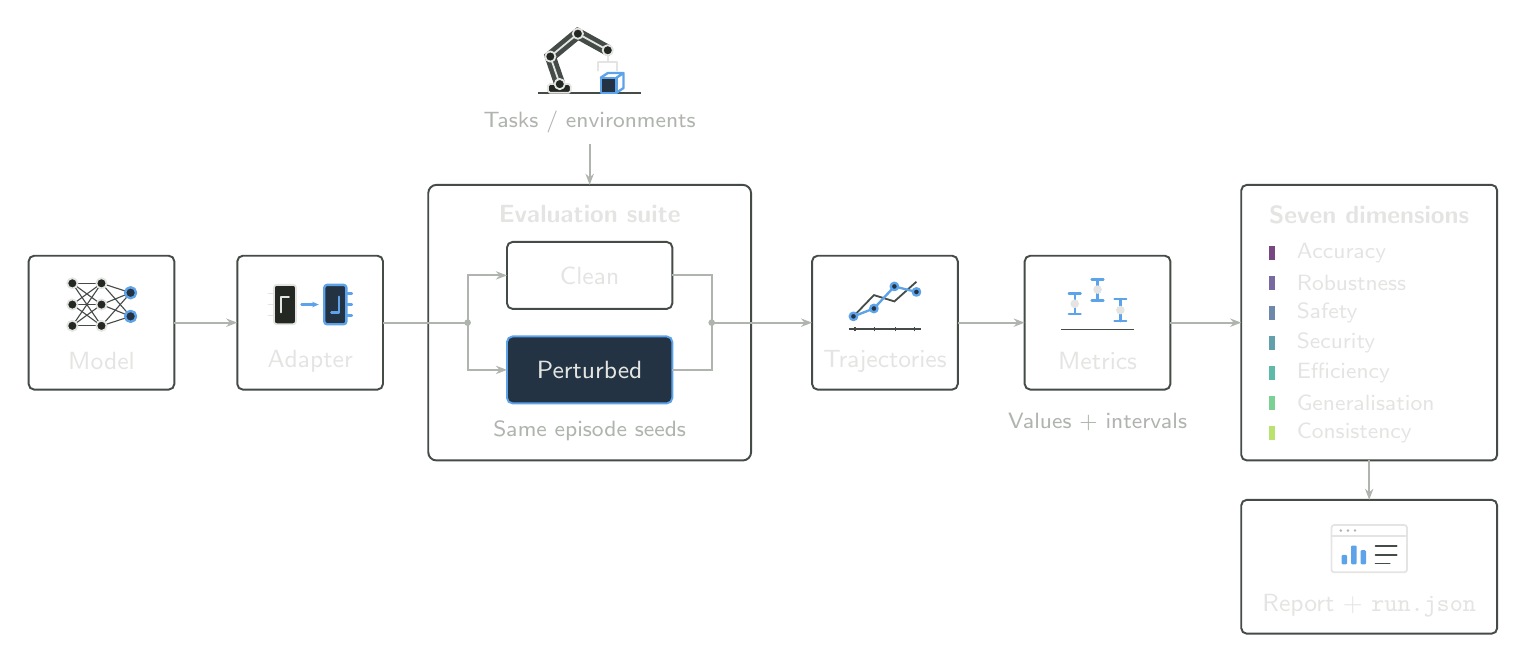
\begin{tikzpicture}[
  x=1cm,y=1cm,
  every node/.style={font=\sffamily\fontsize{9}{11}\selectfont,
    text=ink,inner sep=4pt,outer sep=0pt,align=center},
  box/.style={draw=rule,line width=0.7pt,rounded corners=2pt,
    minimum height=0.85cm,minimum width=1.85cm},
  note/.style={text=muted,font=\sffamily\fontsize{8}{10}\selectfont},
  flow/.style={draw=muted,line width=0.7pt,-{Stealth[length=4pt,width=3pt]}},
  wire/.style={draw=muted,line width=0.7pt},
  icon/.style={draw=ink,line width=0.65pt,line cap=round,line join=round},
  accenticon/.style={draw=signal,line width=0.85pt,line cap=round,line join=round},
  % Small vector illustrations share a two-tone palette and a 0.9 cm footprint.
  pics/model/.style={code={
    \foreach \a in {-0.27,0,0.27} {
      \foreach \b in {-0.27,0,0.27}
        \draw[draw=rule,line width=0.4pt] (-0.37,\a) -- (0,\b);
      \foreach \b in {-0.15,0.15}
        \draw[draw=rule,line width=0.4pt] (0,\a) -- (0.37,\b);
    }
    \foreach \x in {-0.37,0} {
      \foreach \y in {-0.27,0,0.27}
        \draw[icon,fill=panel] (\x,\y) circle (0.065);
    }
    \foreach \y in {-0.15,0.15}
      \draw[accenticon,fill=tint] (0.37,\y) circle (0.07);
  }},
  pics/adapter/.style={code={
    \draw[icon,fill=panel,rounded corners=1pt] (-0.46,-0.25) rectangle (-0.18,0.25);
    \draw[accenticon,fill=tint,rounded corners=1pt] (0.18,-0.25) rectangle (0.46,0.25);
    \foreach \y in {-0.14,0,0.14} {
      \draw[icon] (-0.53,\y) -- (-0.46,\y);
      \draw[accenticon] (0.46,\y) -- (0.53,\y);
    }
    \draw[accenticon,-{Stealth[length=2.4pt,width=2pt]}] (-0.11,0) -- (0.11,0);
    \draw[icon] (-0.37,-0.10) -- (-0.37,0.10) -- (-0.27,0.10);
    \draw[accenticon] (0.27,-0.10) -- (0.37,-0.10) -- (0.37,0.10);
  }},
  pics/trajectory/.style={code={
    \draw[draw=rule,line width=0.45pt] (-0.46,-0.31) -- (0.46,-0.31);
    \foreach \x in {-0.38,-0.13,0.13,0.38}
      \draw[draw=rule,line width=0.45pt] (\x,-0.34) -- (\x,-0.28);
    \draw[draw=rule,line width=0.65pt] (-0.40,-0.15) -- (-0.14,0.12) -- (0.12,0.04) -- (0.40,0.29);
    \draw[accenticon] (-0.40,-0.15) -- (-0.14,-0.05) -- (0.12,0.23) -- (0.40,0.16);
    \foreach \x/\y in {-0.40/-0.15,-0.14/-0.05,0.12/0.23,0.40/0.16}
      \draw[accenticon,fill=tint] (\x,\y) circle (0.047);
  }},
  pics/metrics/.style={code={
    \draw[draw=rule,line width=0.45pt] (-0.46,-0.32) -- (0.46,-0.32);
    \foreach \x/\y/\lo/\hi in {-0.29/0.01/-0.12/0.14,0/0.19/0.05/0.32,0.29/-0.07/-0.21/0.07} {
      \draw[accenticon] (\x,\lo) -- (\x,\hi)
        (\x-0.075,\lo) -- (\x+0.075,\lo)
        (\x-0.075,\hi) -- (\x+0.075,\hi);
      \fill[ink] (\x,\y) circle (0.055);
    }
  }},
  pics/scene/.style={code={
    % Articulated manipulator and an object on its work surface.
    \draw[draw=rule,line width=0.6pt] (-0.65,-0.38) -- (0.65,-0.38);
    \draw[icon,fill=panel,rounded corners=0.7pt] (-0.53,-0.38) rectangle (-0.24,-0.27);
    \draw[draw=rule,line width=4pt,line cap=round] (-0.38,-0.27) -- (-0.50,0.08) -- (-0.15,0.37) -- (0.23,0.16);
    \draw[icon] (-0.38,-0.27) -- (-0.50,0.08) -- (-0.15,0.37) -- (0.23,0.16);
    \foreach \x/\y in {-0.38/-0.27,-0.50/0.08,-0.15/0.37,0.23/0.16}
      \draw[icon,fill=panel] (\x,\y) circle (0.065);
    \draw[icon] (0.23,0.09) -- (0.23,0.01)
      (0.11,-0.10) -- (0.11,0.01) -- (0.35,0.01) -- (0.35,-0.10);
    \draw[accenticon,fill=tint] (0.14,-0.38) rectangle (0.34,-0.19);
    \draw[accenticon] (0.14,-0.19) -- (0.23,-0.13) -- (0.43,-0.13)
      -- (0.34,-0.19) (0.43,-0.13) -- (0.43,-0.32) -- (0.34,-0.38);
  }},
  pics/report/.style={code={
    \draw[icon,rounded corners=1pt] (-0.48,-0.30) rectangle (0.48,0.30);
    \draw[icon] (-0.48,0.16) -- (0.48,0.16);
    \foreach \x in {-0.36,-0.27,-0.18}
      \fill[muted] (\x,0.23) circle (0.018);
    \foreach \x/\h in {-0.35/0.12,-0.23/0.24,-0.11/0.18}
      \fill[signal,rounded corners=0.4pt] (\x,-0.20) rectangle ++(0.07,\h);
    \draw[draw=rule,line width=0.6pt,line cap=round]
      (0.08,0.03) -- (0.35,0.03) (0.08,-0.08) -- (0.35,-0.08)
      (0.08,-0.19) -- (0.26,-0.19);
  }},
]
% The suite branches into matched conditions, whose recorded trajectories feed
% the same metrics. Boxes denote operations or data, never illustrative scores.
\node[box,minimum height=1.70cm] (model) at (0,0) {};
\pic at (0,0.23) {model};
\node at (0,-0.49) {Model};
\node[box,minimum height=1.70cm] (adapter) at (2.65,0) {};
\pic at (2.65,0.23) {adapter};
\node at (2.65,-0.49) {Adapter};
\draw[flow] (model) -- (adapter);

\draw[draw=rule,line width=0.7pt,rounded corners=3pt]
  (4.15,-1.75) rectangle (8.25,1.75);
\node[font=\sffamily\bfseries\fontsize{9}{11}\selectfont]
  at (6.20,1.38) {Evaluation suite};
\node[box,minimum width=2.1cm] (clean) at (6.20,0.60) {Clean};
\node[box,minimum width=2.1cm,draw=signal,fill=tint]
  (perturbed) at (6.20,-0.60) {Perturbed};
\node[note] at (6.20,-1.38) {Same episode seeds};
\coordinate (split) at (4.65,0);
\draw[wire] (adapter.east) -- (split);
\draw[flow] (split) |- (clean.west);
\draw[flow] (split) |- (perturbed.west);
\fill[muted] (split) circle (1.2pt);

\pic at (6.20,3.30) {scene};
\node[note] (tasks) at (6.20,2.55) {Tasks / environments};
\draw[flow] (tasks.south) -- (6.20,1.75);

\node[box,minimum height=1.70cm] (trajectories) at (9.95,0) {};
\pic at (9.95,0.23) {trajectory};
\node at (9.95,-0.49) {Trajectories};
\coordinate (join) at (7.75,0);
\draw[wire] (clean.east) -| (join);
\draw[wire] (perturbed.east) -| (join);
\draw[flow] (join) -- (trajectories.west);
\fill[muted] (join) circle (1.2pt);
\node[box,minimum height=1.70cm] (metrics) at (12.65,0) {};
\pic at (12.65,0.23) {metrics};
\node at (12.65,-0.49) {Metrics};
\draw[flow] (trajectories) -- (metrics);
\node[note,anchor=north] at (12.65,-1.01) {Values + intervals};

% A compact, named output vector avoids fabricating a chart of model scores.
\node[box,minimum width=3.25cm,minimum height=3.50cm]
  (profile) at (16.10,0) {};
\node[font=\sffamily\bfseries\fontsize{9}{11}\selectfont]
  at (16.10,1.37) {Seven dimensions};
\foreach \y/\col/\title in {
  0.88/dimA/Accuracy,
  0.50/dimB/Robustness,
  0.12/dimC/Safety,
  -0.26/dimD/Security,
  -0.64/dimE/Efficiency,
  -1.02/dimF/Generalisation,
  -1.40/dimG/Consistency} {
  \fill[\col] (14.83,\y-0.09) rectangle ++(0.07,0.18);
  \node[anchor=west,font=\sffamily\fontsize{8.5}{10}\selectfont]
    at (15.04,\y) {\title};
}
\draw[flow] (metrics) -- (profile);
\node[box,minimum width=3.25cm,minimum height=1.70cm] (artifacts) at (16.10,-3.10) {};
\pic at (16.10,-2.87) {report};
\node at (16.10,-3.59) {Report + \texttt{run.json}};
\draw[flow] (profile) -- (artifacts);
\end{tikzpicture}
\end{document}
"
%   pdftocairo -svg method-light.pdf method-light.svg
%   pdftocairo -svg method-dark.pdf method-dark.svg
% Commit the SVGs; documentation builds do not require LaTeX.
\documentclass[border=8pt]{standalone}
\usepackage[T1]{fontenc}
\usepackage{lmodern}
\usepackage{xcolor}
\usepackage{tikz}
\usetikzlibrary{arrows.meta}
\providecommand{\xevalstheme}{light}
\def\xevalslight{light}
\ifx\xevalstheme\xevalslight
  \definecolor{ink}{HTML}{121412}
  \definecolor{muted}{HTML}{5C615D}
  \definecolor{rule}{HTML}{A8ADA7}
  \definecolor{panel}{HTML}{F1F2EF}
  \definecolor{signal}{HTML}{367FC9}
  \definecolor{tint}{HTML}{E8F0F8}
  \definecolor{dimA}{HTML}{440154}\definecolor{dimB}{HTML}{46327E}
  \definecolor{dimC}{HTML}{365C8D}\definecolor{dimD}{HTML}{277F8E}
  \definecolor{dimE}{HTML}{1FA187}\definecolor{dimF}{HTML}{4AC16D}
  \definecolor{dimG}{HTML}{A0DA39}
\else
  \definecolor{ink}{HTML}{E4E5E2}
  \definecolor{muted}{HTML}{AFB4AE}
  \definecolor{rule}{HTML}{454B46}
  \definecolor{panel}{HTML}{232823}
  \definecolor{signal}{HTML}{5DA3E9}
  \definecolor{tint}{HTML}{233344}
  \definecolor{dimA}{HTML}{774782}\definecolor{dimB}{HTML}{786AA0}
  \definecolor{dimC}{HTML}{6D88AB}\definecolor{dimD}{HTML}{62A1AC}
  \definecolor{dimE}{HTML}{5CBAA7}\definecolor{dimF}{HTML}{7BD194}
  \definecolor{dimG}{HTML}{B9E36E}
\fi
\begin{document}
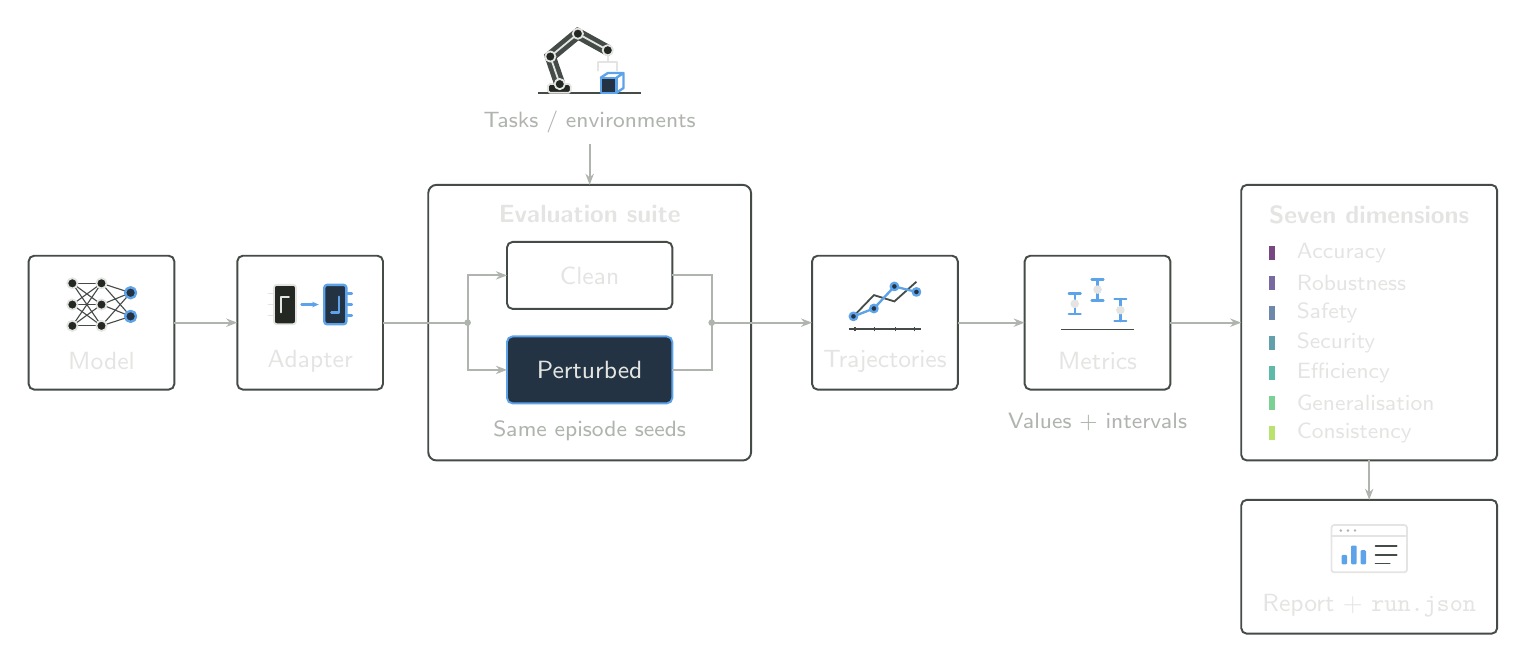
\begin{tikzpicture}[
  x=1cm,y=1cm,
  every node/.style={font=\sffamily\fontsize{9}{11}\selectfont,
    text=ink,inner sep=4pt,outer sep=0pt,align=center},
  box/.style={draw=rule,line width=0.7pt,rounded corners=2pt,
    minimum height=0.85cm,minimum width=1.85cm},
  note/.style={text=muted,font=\sffamily\fontsize{8}{10}\selectfont},
  flow/.style={draw=muted,line width=0.7pt,-{Stealth[length=4pt,width=3pt]}},
  wire/.style={draw=muted,line width=0.7pt},
  icon/.style={draw=ink,line width=0.65pt,line cap=round,line join=round},
  accenticon/.style={draw=signal,line width=0.85pt,line cap=round,line join=round},
  % Small vector illustrations share a two-tone palette and a 0.9 cm footprint.
  pics/model/.style={code={
    \foreach \a in {-0.27,0,0.27} {
      \foreach \b in {-0.27,0,0.27}
        \draw[draw=rule,line width=0.4pt] (-0.37,\a) -- (0,\b);
      \foreach \b in {-0.15,0.15}
        \draw[draw=rule,line width=0.4pt] (0,\a) -- (0.37,\b);
    }
    \foreach \x in {-0.37,0} {
      \foreach \y in {-0.27,0,0.27}
        \draw[icon,fill=panel] (\x,\y) circle (0.065);
    }
    \foreach \y in {-0.15,0.15}
      \draw[accenticon,fill=tint] (0.37,\y) circle (0.07);
  }},
  pics/adapter/.style={code={
    \draw[icon,fill=panel,rounded corners=1pt] (-0.46,-0.25) rectangle (-0.18,0.25);
    \draw[accenticon,fill=tint,rounded corners=1pt] (0.18,-0.25) rectangle (0.46,0.25);
    \foreach \y in {-0.14,0,0.14} {
      \draw[icon] (-0.53,\y) -- (-0.46,\y);
      \draw[accenticon] (0.46,\y) -- (0.53,\y);
    }
    \draw[accenticon,-{Stealth[length=2.4pt,width=2pt]}] (-0.11,0) -- (0.11,0);
    \draw[icon] (-0.37,-0.10) -- (-0.37,0.10) -- (-0.27,0.10);
    \draw[accenticon] (0.27,-0.10) -- (0.37,-0.10) -- (0.37,0.10);
  }},
  pics/trajectory/.style={code={
    \draw[draw=rule,line width=0.45pt] (-0.46,-0.31) -- (0.46,-0.31);
    \foreach \x in {-0.38,-0.13,0.13,0.38}
      \draw[draw=rule,line width=0.45pt] (\x,-0.34) -- (\x,-0.28);
    \draw[draw=rule,line width=0.65pt] (-0.40,-0.15) -- (-0.14,0.12) -- (0.12,0.04) -- (0.40,0.29);
    \draw[accenticon] (-0.40,-0.15) -- (-0.14,-0.05) -- (0.12,0.23) -- (0.40,0.16);
    \foreach \x/\y in {-0.40/-0.15,-0.14/-0.05,0.12/0.23,0.40/0.16}
      \draw[accenticon,fill=tint] (\x,\y) circle (0.047);
  }},
  pics/metrics/.style={code={
    \draw[draw=rule,line width=0.45pt] (-0.46,-0.32) -- (0.46,-0.32);
    \foreach \x/\y/\lo/\hi in {-0.29/0.01/-0.12/0.14,0/0.19/0.05/0.32,0.29/-0.07/-0.21/0.07} {
      \draw[accenticon] (\x,\lo) -- (\x,\hi)
        (\x-0.075,\lo) -- (\x+0.075,\lo)
        (\x-0.075,\hi) -- (\x+0.075,\hi);
      \fill[ink] (\x,\y) circle (0.055);
    }
  }},
  pics/scene/.style={code={
    % Articulated manipulator and an object on its work surface.
    \draw[draw=rule,line width=0.6pt] (-0.65,-0.38) -- (0.65,-0.38);
    \draw[icon,fill=panel,rounded corners=0.7pt] (-0.53,-0.38) rectangle (-0.24,-0.27);
    \draw[draw=rule,line width=4pt,line cap=round] (-0.38,-0.27) -- (-0.50,0.08) -- (-0.15,0.37) -- (0.23,0.16);
    \draw[icon] (-0.38,-0.27) -- (-0.50,0.08) -- (-0.15,0.37) -- (0.23,0.16);
    \foreach \x/\y in {-0.38/-0.27,-0.50/0.08,-0.15/0.37,0.23/0.16}
      \draw[icon,fill=panel] (\x,\y) circle (0.065);
    \draw[icon] (0.23,0.09) -- (0.23,0.01)
      (0.11,-0.10) -- (0.11,0.01) -- (0.35,0.01) -- (0.35,-0.10);
    \draw[accenticon,fill=tint] (0.14,-0.38) rectangle (0.34,-0.19);
    \draw[accenticon] (0.14,-0.19) -- (0.23,-0.13) -- (0.43,-0.13)
      -- (0.34,-0.19) (0.43,-0.13) -- (0.43,-0.32) -- (0.34,-0.38);
  }},
  pics/report/.style={code={
    \draw[icon,rounded corners=1pt] (-0.48,-0.30) rectangle (0.48,0.30);
    \draw[icon] (-0.48,0.16) -- (0.48,0.16);
    \foreach \x in {-0.36,-0.27,-0.18}
      \fill[muted] (\x,0.23) circle (0.018);
    \foreach \x/\h in {-0.35/0.12,-0.23/0.24,-0.11/0.18}
      \fill[signal,rounded corners=0.4pt] (\x,-0.20) rectangle ++(0.07,\h);
    \draw[draw=rule,line width=0.6pt,line cap=round]
      (0.08,0.03) -- (0.35,0.03) (0.08,-0.08) -- (0.35,-0.08)
      (0.08,-0.19) -- (0.26,-0.19);
  }},
]
% The suite branches into matched conditions, whose recorded trajectories feed
% the same metrics. Boxes denote operations or data, never illustrative scores.
\node[box,minimum height=1.70cm] (model) at (0,0) {};
\pic at (0,0.23) {model};
\node at (0,-0.49) {Model};
\node[box,minimum height=1.70cm] (adapter) at (2.65,0) {};
\pic at (2.65,0.23) {adapter};
\node at (2.65,-0.49) {Adapter};
\draw[flow] (model) -- (adapter);

\draw[draw=rule,line width=0.7pt,rounded corners=3pt]
  (4.15,-1.75) rectangle (8.25,1.75);
\node[font=\sffamily\bfseries\fontsize{9}{11}\selectfont]
  at (6.20,1.38) {Evaluation suite};
\node[box,minimum width=2.1cm] (clean) at (6.20,0.60) {Clean};
\node[box,minimum width=2.1cm,draw=signal,fill=tint]
  (perturbed) at (6.20,-0.60) {Perturbed};
\node[note] at (6.20,-1.38) {Same episode seeds};
\coordinate (split) at (4.65,0);
\draw[wire] (adapter.east) -- (split);
\draw[flow] (split) |- (clean.west);
\draw[flow] (split) |- (perturbed.west);
\fill[muted] (split) circle (1.2pt);

\pic at (6.20,3.30) {scene};
\node[note] (tasks) at (6.20,2.55) {Tasks / environments};
\draw[flow] (tasks.south) -- (6.20,1.75);

\node[box,minimum height=1.70cm] (trajectories) at (9.95,0) {};
\pic at (9.95,0.23) {trajectory};
\node at (9.95,-0.49) {Trajectories};
\coordinate (join) at (7.75,0);
\draw[wire] (clean.east) -| (join);
\draw[wire] (perturbed.east) -| (join);
\draw[flow] (join) -- (trajectories.west);
\fill[muted] (join) circle (1.2pt);
\node[box,minimum height=1.70cm] (metrics) at (12.65,0) {};
\pic at (12.65,0.23) {metrics};
\node at (12.65,-0.49) {Metrics};
\draw[flow] (trajectories) -- (metrics);
\node[note,anchor=north] at (12.65,-1.01) {Values + intervals};

% A compact, named output vector avoids fabricating a chart of model scores.
\node[box,minimum width=3.25cm,minimum height=3.50cm]
  (profile) at (16.10,0) {};
\node[font=\sffamily\bfseries\fontsize{9}{11}\selectfont]
  at (16.10,1.37) {Seven dimensions};
\foreach \y/\col/\title in {
  0.88/dimA/Accuracy,
  0.50/dimB/Robustness,
  0.12/dimC/Safety,
  -0.26/dimD/Security,
  -0.64/dimE/Efficiency,
  -1.02/dimF/Generalisation,
  -1.40/dimG/Consistency} {
  \fill[\col] (14.83,\y-0.09) rectangle ++(0.07,0.18);
  \node[anchor=west,font=\sffamily\fontsize{8.5}{10}\selectfont]
    at (15.04,\y) {\title};
}
\draw[flow] (metrics) -- (profile);
\node[box,minimum width=3.25cm,minimum height=1.70cm] (artifacts) at (16.10,-3.10) {};
\pic at (16.10,-2.87) {report};
\node at (16.10,-3.59) {Report + \texttt{run.json}};
\draw[flow] (profile) -- (artifacts);
\end{tikzpicture}
\end{document}
"
%   pdflatex -jobname=method-dark  "\def\xevalstheme{dark}% Documentation method diagram. Build both themes with TeX Live and poppler:
%   pdflatex -jobname=method-light "\def\xevalstheme{light}% Documentation method diagram. Build both themes with TeX Live and poppler:
%   pdflatex -jobname=method-light "\def\xevalstheme{light}% Documentation method diagram. Build both themes with TeX Live and poppler:
%   pdflatex -jobname=method-light "\def\xevalstheme{light}\input{method.tex}"
%   pdflatex -jobname=method-dark  "\def\xevalstheme{dark}\input{method.tex}"
%   pdftocairo -svg method-light.pdf method-light.svg
%   pdftocairo -svg method-dark.pdf method-dark.svg
% Commit the SVGs; documentation builds do not require LaTeX.
\documentclass[border=8pt]{standalone}
\usepackage[T1]{fontenc}
\usepackage{lmodern}
\usepackage{xcolor}
\usepackage{tikz}
\usetikzlibrary{arrows.meta}
\providecommand{\xevalstheme}{light}
\def\xevalslight{light}
\ifx\xevalstheme\xevalslight
  \definecolor{ink}{HTML}{121412}
  \definecolor{muted}{HTML}{5C615D}
  \definecolor{rule}{HTML}{A8ADA7}
  \definecolor{panel}{HTML}{F1F2EF}
  \definecolor{signal}{HTML}{367FC9}
  \definecolor{tint}{HTML}{E8F0F8}
  \definecolor{dimA}{HTML}{440154}\definecolor{dimB}{HTML}{46327E}
  \definecolor{dimC}{HTML}{365C8D}\definecolor{dimD}{HTML}{277F8E}
  \definecolor{dimE}{HTML}{1FA187}\definecolor{dimF}{HTML}{4AC16D}
  \definecolor{dimG}{HTML}{A0DA39}
\else
  \definecolor{ink}{HTML}{E4E5E2}
  \definecolor{muted}{HTML}{AFB4AE}
  \definecolor{rule}{HTML}{454B46}
  \definecolor{panel}{HTML}{232823}
  \definecolor{signal}{HTML}{5DA3E9}
  \definecolor{tint}{HTML}{233344}
  \definecolor{dimA}{HTML}{774782}\definecolor{dimB}{HTML}{786AA0}
  \definecolor{dimC}{HTML}{6D88AB}\definecolor{dimD}{HTML}{62A1AC}
  \definecolor{dimE}{HTML}{5CBAA7}\definecolor{dimF}{HTML}{7BD194}
  \definecolor{dimG}{HTML}{B9E36E}
\fi
\begin{document}
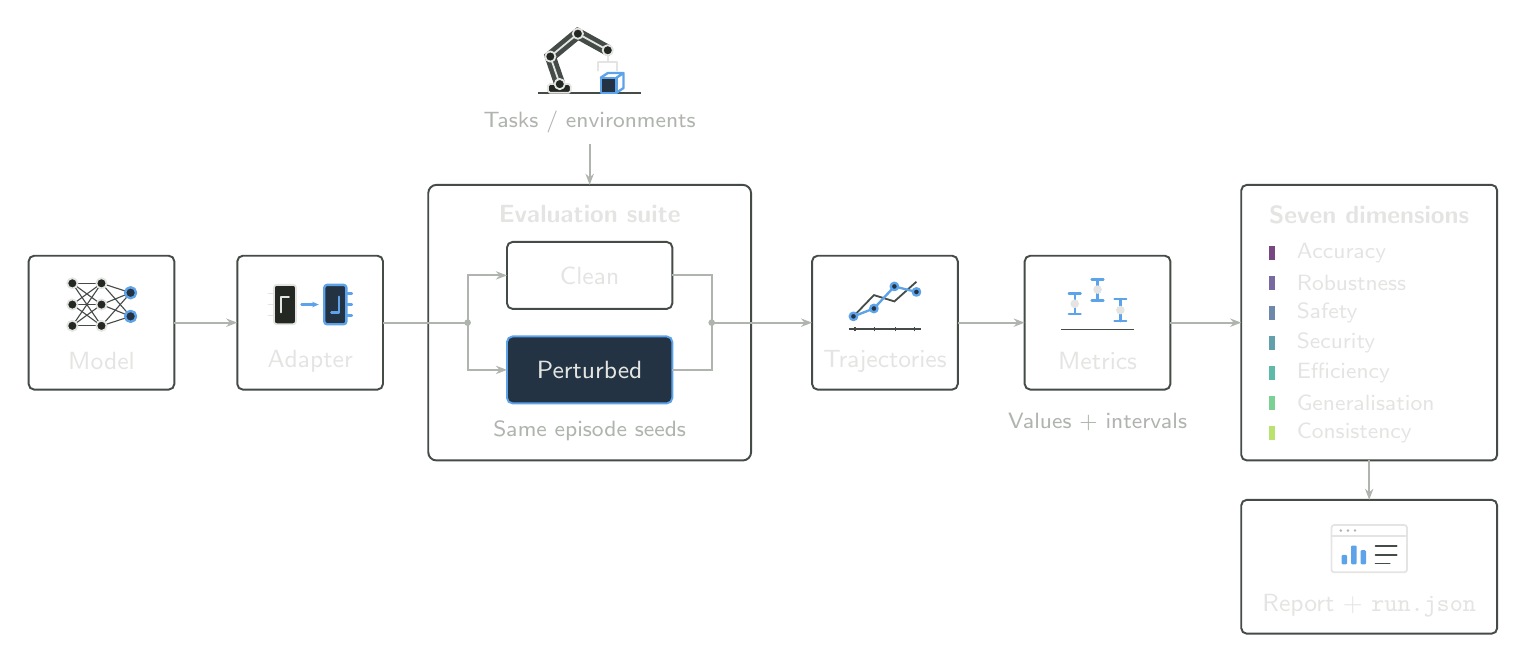
\begin{tikzpicture}[
  x=1cm,y=1cm,
  every node/.style={font=\sffamily\fontsize{9}{11}\selectfont,
    text=ink,inner sep=4pt,outer sep=0pt,align=center},
  box/.style={draw=rule,line width=0.7pt,rounded corners=2pt,
    minimum height=0.85cm,minimum width=1.85cm},
  note/.style={text=muted,font=\sffamily\fontsize{8}{10}\selectfont},
  flow/.style={draw=muted,line width=0.7pt,-{Stealth[length=4pt,width=3pt]}},
  wire/.style={draw=muted,line width=0.7pt},
  icon/.style={draw=ink,line width=0.65pt,line cap=round,line join=round},
  accenticon/.style={draw=signal,line width=0.85pt,line cap=round,line join=round},
  % Small vector illustrations share a two-tone palette and a 0.9 cm footprint.
  pics/model/.style={code={
    \foreach \a in {-0.27,0,0.27} {
      \foreach \b in {-0.27,0,0.27}
        \draw[draw=rule,line width=0.4pt] (-0.37,\a) -- (0,\b);
      \foreach \b in {-0.15,0.15}
        \draw[draw=rule,line width=0.4pt] (0,\a) -- (0.37,\b);
    }
    \foreach \x in {-0.37,0} {
      \foreach \y in {-0.27,0,0.27}
        \draw[icon,fill=panel] (\x,\y) circle (0.065);
    }
    \foreach \y in {-0.15,0.15}
      \draw[accenticon,fill=tint] (0.37,\y) circle (0.07);
  }},
  pics/adapter/.style={code={
    \draw[icon,fill=panel,rounded corners=1pt] (-0.46,-0.25) rectangle (-0.18,0.25);
    \draw[accenticon,fill=tint,rounded corners=1pt] (0.18,-0.25) rectangle (0.46,0.25);
    \foreach \y in {-0.14,0,0.14} {
      \draw[icon] (-0.53,\y) -- (-0.46,\y);
      \draw[accenticon] (0.46,\y) -- (0.53,\y);
    }
    \draw[accenticon,-{Stealth[length=2.4pt,width=2pt]}] (-0.11,0) -- (0.11,0);
    \draw[icon] (-0.37,-0.10) -- (-0.37,0.10) -- (-0.27,0.10);
    \draw[accenticon] (0.27,-0.10) -- (0.37,-0.10) -- (0.37,0.10);
  }},
  pics/trajectory/.style={code={
    \draw[draw=rule,line width=0.45pt] (-0.46,-0.31) -- (0.46,-0.31);
    \foreach \x in {-0.38,-0.13,0.13,0.38}
      \draw[draw=rule,line width=0.45pt] (\x,-0.34) -- (\x,-0.28);
    \draw[draw=rule,line width=0.65pt] (-0.40,-0.15) -- (-0.14,0.12) -- (0.12,0.04) -- (0.40,0.29);
    \draw[accenticon] (-0.40,-0.15) -- (-0.14,-0.05) -- (0.12,0.23) -- (0.40,0.16);
    \foreach \x/\y in {-0.40/-0.15,-0.14/-0.05,0.12/0.23,0.40/0.16}
      \draw[accenticon,fill=tint] (\x,\y) circle (0.047);
  }},
  pics/metrics/.style={code={
    \draw[draw=rule,line width=0.45pt] (-0.46,-0.32) -- (0.46,-0.32);
    \foreach \x/\y/\lo/\hi in {-0.29/0.01/-0.12/0.14,0/0.19/0.05/0.32,0.29/-0.07/-0.21/0.07} {
      \draw[accenticon] (\x,\lo) -- (\x,\hi)
        (\x-0.075,\lo) -- (\x+0.075,\lo)
        (\x-0.075,\hi) -- (\x+0.075,\hi);
      \fill[ink] (\x,\y) circle (0.055);
    }
  }},
  pics/scene/.style={code={
    % Articulated manipulator and an object on its work surface.
    \draw[draw=rule,line width=0.6pt] (-0.65,-0.38) -- (0.65,-0.38);
    \draw[icon,fill=panel,rounded corners=0.7pt] (-0.53,-0.38) rectangle (-0.24,-0.27);
    \draw[draw=rule,line width=4pt,line cap=round] (-0.38,-0.27) -- (-0.50,0.08) -- (-0.15,0.37) -- (0.23,0.16);
    \draw[icon] (-0.38,-0.27) -- (-0.50,0.08) -- (-0.15,0.37) -- (0.23,0.16);
    \foreach \x/\y in {-0.38/-0.27,-0.50/0.08,-0.15/0.37,0.23/0.16}
      \draw[icon,fill=panel] (\x,\y) circle (0.065);
    \draw[icon] (0.23,0.09) -- (0.23,0.01)
      (0.11,-0.10) -- (0.11,0.01) -- (0.35,0.01) -- (0.35,-0.10);
    \draw[accenticon,fill=tint] (0.14,-0.38) rectangle (0.34,-0.19);
    \draw[accenticon] (0.14,-0.19) -- (0.23,-0.13) -- (0.43,-0.13)
      -- (0.34,-0.19) (0.43,-0.13) -- (0.43,-0.32) -- (0.34,-0.38);
  }},
  pics/report/.style={code={
    \draw[icon,rounded corners=1pt] (-0.48,-0.30) rectangle (0.48,0.30);
    \draw[icon] (-0.48,0.16) -- (0.48,0.16);
    \foreach \x in {-0.36,-0.27,-0.18}
      \fill[muted] (\x,0.23) circle (0.018);
    \foreach \x/\h in {-0.35/0.12,-0.23/0.24,-0.11/0.18}
      \fill[signal,rounded corners=0.4pt] (\x,-0.20) rectangle ++(0.07,\h);
    \draw[draw=rule,line width=0.6pt,line cap=round]
      (0.08,0.03) -- (0.35,0.03) (0.08,-0.08) -- (0.35,-0.08)
      (0.08,-0.19) -- (0.26,-0.19);
  }},
]
% The suite branches into matched conditions, whose recorded trajectories feed
% the same metrics. Boxes denote operations or data, never illustrative scores.
\node[box,minimum height=1.70cm] (model) at (0,0) {};
\pic at (0,0.23) {model};
\node at (0,-0.49) {Model};
\node[box,minimum height=1.70cm] (adapter) at (2.65,0) {};
\pic at (2.65,0.23) {adapter};
\node at (2.65,-0.49) {Adapter};
\draw[flow] (model) -- (adapter);

\draw[draw=rule,line width=0.7pt,rounded corners=3pt]
  (4.15,-1.75) rectangle (8.25,1.75);
\node[font=\sffamily\bfseries\fontsize{9}{11}\selectfont]
  at (6.20,1.38) {Evaluation suite};
\node[box,minimum width=2.1cm] (clean) at (6.20,0.60) {Clean};
\node[box,minimum width=2.1cm,draw=signal,fill=tint]
  (perturbed) at (6.20,-0.60) {Perturbed};
\node[note] at (6.20,-1.38) {Same episode seeds};
\coordinate (split) at (4.65,0);
\draw[wire] (adapter.east) -- (split);
\draw[flow] (split) |- (clean.west);
\draw[flow] (split) |- (perturbed.west);
\fill[muted] (split) circle (1.2pt);

\pic at (6.20,3.30) {scene};
\node[note] (tasks) at (6.20,2.55) {Tasks / environments};
\draw[flow] (tasks.south) -- (6.20,1.75);

\node[box,minimum height=1.70cm] (trajectories) at (9.95,0) {};
\pic at (9.95,0.23) {trajectory};
\node at (9.95,-0.49) {Trajectories};
\coordinate (join) at (7.75,0);
\draw[wire] (clean.east) -| (join);
\draw[wire] (perturbed.east) -| (join);
\draw[flow] (join) -- (trajectories.west);
\fill[muted] (join) circle (1.2pt);
\node[box,minimum height=1.70cm] (metrics) at (12.65,0) {};
\pic at (12.65,0.23) {metrics};
\node at (12.65,-0.49) {Metrics};
\draw[flow] (trajectories) -- (metrics);
\node[note,anchor=north] at (12.65,-1.01) {Values + intervals};

% A compact, named output vector avoids fabricating a chart of model scores.
\node[box,minimum width=3.25cm,minimum height=3.50cm]
  (profile) at (16.10,0) {};
\node[font=\sffamily\bfseries\fontsize{9}{11}\selectfont]
  at (16.10,1.37) {Seven dimensions};
\foreach \y/\col/\title in {
  0.88/dimA/Accuracy,
  0.50/dimB/Robustness,
  0.12/dimC/Safety,
  -0.26/dimD/Security,
  -0.64/dimE/Efficiency,
  -1.02/dimF/Generalisation,
  -1.40/dimG/Consistency} {
  \fill[\col] (14.83,\y-0.09) rectangle ++(0.07,0.18);
  \node[anchor=west,font=\sffamily\fontsize{8.5}{10}\selectfont]
    at (15.04,\y) {\title};
}
\draw[flow] (metrics) -- (profile);
\node[box,minimum width=3.25cm,minimum height=1.70cm] (artifacts) at (16.10,-3.10) {};
\pic at (16.10,-2.87) {report};
\node at (16.10,-3.59) {Report + \texttt{run.json}};
\draw[flow] (profile) -- (artifacts);
\end{tikzpicture}
\end{document}
"
%   pdflatex -jobname=method-dark  "\def\xevalstheme{dark}% Documentation method diagram. Build both themes with TeX Live and poppler:
%   pdflatex -jobname=method-light "\def\xevalstheme{light}\input{method.tex}"
%   pdflatex -jobname=method-dark  "\def\xevalstheme{dark}\input{method.tex}"
%   pdftocairo -svg method-light.pdf method-light.svg
%   pdftocairo -svg method-dark.pdf method-dark.svg
% Commit the SVGs; documentation builds do not require LaTeX.
\documentclass[border=8pt]{standalone}
\usepackage[T1]{fontenc}
\usepackage{lmodern}
\usepackage{xcolor}
\usepackage{tikz}
\usetikzlibrary{arrows.meta}
\providecommand{\xevalstheme}{light}
\def\xevalslight{light}
\ifx\xevalstheme\xevalslight
  \definecolor{ink}{HTML}{121412}
  \definecolor{muted}{HTML}{5C615D}
  \definecolor{rule}{HTML}{A8ADA7}
  \definecolor{panel}{HTML}{F1F2EF}
  \definecolor{signal}{HTML}{367FC9}
  \definecolor{tint}{HTML}{E8F0F8}
  \definecolor{dimA}{HTML}{440154}\definecolor{dimB}{HTML}{46327E}
  \definecolor{dimC}{HTML}{365C8D}\definecolor{dimD}{HTML}{277F8E}
  \definecolor{dimE}{HTML}{1FA187}\definecolor{dimF}{HTML}{4AC16D}
  \definecolor{dimG}{HTML}{A0DA39}
\else
  \definecolor{ink}{HTML}{E4E5E2}
  \definecolor{muted}{HTML}{AFB4AE}
  \definecolor{rule}{HTML}{454B46}
  \definecolor{panel}{HTML}{232823}
  \definecolor{signal}{HTML}{5DA3E9}
  \definecolor{tint}{HTML}{233344}
  \definecolor{dimA}{HTML}{774782}\definecolor{dimB}{HTML}{786AA0}
  \definecolor{dimC}{HTML}{6D88AB}\definecolor{dimD}{HTML}{62A1AC}
  \definecolor{dimE}{HTML}{5CBAA7}\definecolor{dimF}{HTML}{7BD194}
  \definecolor{dimG}{HTML}{B9E36E}
\fi
\begin{document}
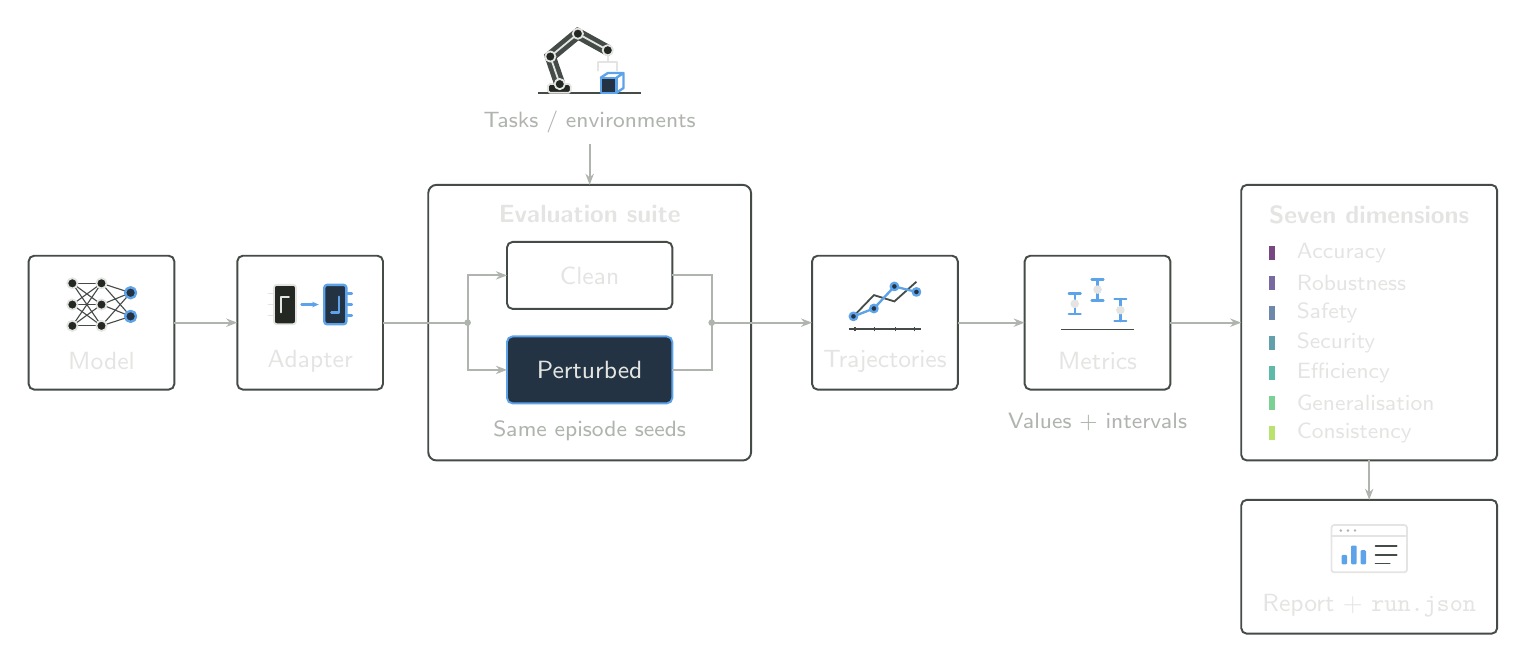
\begin{tikzpicture}[
  x=1cm,y=1cm,
  every node/.style={font=\sffamily\fontsize{9}{11}\selectfont,
    text=ink,inner sep=4pt,outer sep=0pt,align=center},
  box/.style={draw=rule,line width=0.7pt,rounded corners=2pt,
    minimum height=0.85cm,minimum width=1.85cm},
  note/.style={text=muted,font=\sffamily\fontsize{8}{10}\selectfont},
  flow/.style={draw=muted,line width=0.7pt,-{Stealth[length=4pt,width=3pt]}},
  wire/.style={draw=muted,line width=0.7pt},
  icon/.style={draw=ink,line width=0.65pt,line cap=round,line join=round},
  accenticon/.style={draw=signal,line width=0.85pt,line cap=round,line join=round},
  % Small vector illustrations share a two-tone palette and a 0.9 cm footprint.
  pics/model/.style={code={
    \foreach \a in {-0.27,0,0.27} {
      \foreach \b in {-0.27,0,0.27}
        \draw[draw=rule,line width=0.4pt] (-0.37,\a) -- (0,\b);
      \foreach \b in {-0.15,0.15}
        \draw[draw=rule,line width=0.4pt] (0,\a) -- (0.37,\b);
    }
    \foreach \x in {-0.37,0} {
      \foreach \y in {-0.27,0,0.27}
        \draw[icon,fill=panel] (\x,\y) circle (0.065);
    }
    \foreach \y in {-0.15,0.15}
      \draw[accenticon,fill=tint] (0.37,\y) circle (0.07);
  }},
  pics/adapter/.style={code={
    \draw[icon,fill=panel,rounded corners=1pt] (-0.46,-0.25) rectangle (-0.18,0.25);
    \draw[accenticon,fill=tint,rounded corners=1pt] (0.18,-0.25) rectangle (0.46,0.25);
    \foreach \y in {-0.14,0,0.14} {
      \draw[icon] (-0.53,\y) -- (-0.46,\y);
      \draw[accenticon] (0.46,\y) -- (0.53,\y);
    }
    \draw[accenticon,-{Stealth[length=2.4pt,width=2pt]}] (-0.11,0) -- (0.11,0);
    \draw[icon] (-0.37,-0.10) -- (-0.37,0.10) -- (-0.27,0.10);
    \draw[accenticon] (0.27,-0.10) -- (0.37,-0.10) -- (0.37,0.10);
  }},
  pics/trajectory/.style={code={
    \draw[draw=rule,line width=0.45pt] (-0.46,-0.31) -- (0.46,-0.31);
    \foreach \x in {-0.38,-0.13,0.13,0.38}
      \draw[draw=rule,line width=0.45pt] (\x,-0.34) -- (\x,-0.28);
    \draw[draw=rule,line width=0.65pt] (-0.40,-0.15) -- (-0.14,0.12) -- (0.12,0.04) -- (0.40,0.29);
    \draw[accenticon] (-0.40,-0.15) -- (-0.14,-0.05) -- (0.12,0.23) -- (0.40,0.16);
    \foreach \x/\y in {-0.40/-0.15,-0.14/-0.05,0.12/0.23,0.40/0.16}
      \draw[accenticon,fill=tint] (\x,\y) circle (0.047);
  }},
  pics/metrics/.style={code={
    \draw[draw=rule,line width=0.45pt] (-0.46,-0.32) -- (0.46,-0.32);
    \foreach \x/\y/\lo/\hi in {-0.29/0.01/-0.12/0.14,0/0.19/0.05/0.32,0.29/-0.07/-0.21/0.07} {
      \draw[accenticon] (\x,\lo) -- (\x,\hi)
        (\x-0.075,\lo) -- (\x+0.075,\lo)
        (\x-0.075,\hi) -- (\x+0.075,\hi);
      \fill[ink] (\x,\y) circle (0.055);
    }
  }},
  pics/scene/.style={code={
    % Articulated manipulator and an object on its work surface.
    \draw[draw=rule,line width=0.6pt] (-0.65,-0.38) -- (0.65,-0.38);
    \draw[icon,fill=panel,rounded corners=0.7pt] (-0.53,-0.38) rectangle (-0.24,-0.27);
    \draw[draw=rule,line width=4pt,line cap=round] (-0.38,-0.27) -- (-0.50,0.08) -- (-0.15,0.37) -- (0.23,0.16);
    \draw[icon] (-0.38,-0.27) -- (-0.50,0.08) -- (-0.15,0.37) -- (0.23,0.16);
    \foreach \x/\y in {-0.38/-0.27,-0.50/0.08,-0.15/0.37,0.23/0.16}
      \draw[icon,fill=panel] (\x,\y) circle (0.065);
    \draw[icon] (0.23,0.09) -- (0.23,0.01)
      (0.11,-0.10) -- (0.11,0.01) -- (0.35,0.01) -- (0.35,-0.10);
    \draw[accenticon,fill=tint] (0.14,-0.38) rectangle (0.34,-0.19);
    \draw[accenticon] (0.14,-0.19) -- (0.23,-0.13) -- (0.43,-0.13)
      -- (0.34,-0.19) (0.43,-0.13) -- (0.43,-0.32) -- (0.34,-0.38);
  }},
  pics/report/.style={code={
    \draw[icon,rounded corners=1pt] (-0.48,-0.30) rectangle (0.48,0.30);
    \draw[icon] (-0.48,0.16) -- (0.48,0.16);
    \foreach \x in {-0.36,-0.27,-0.18}
      \fill[muted] (\x,0.23) circle (0.018);
    \foreach \x/\h in {-0.35/0.12,-0.23/0.24,-0.11/0.18}
      \fill[signal,rounded corners=0.4pt] (\x,-0.20) rectangle ++(0.07,\h);
    \draw[draw=rule,line width=0.6pt,line cap=round]
      (0.08,0.03) -- (0.35,0.03) (0.08,-0.08) -- (0.35,-0.08)
      (0.08,-0.19) -- (0.26,-0.19);
  }},
]
% The suite branches into matched conditions, whose recorded trajectories feed
% the same metrics. Boxes denote operations or data, never illustrative scores.
\node[box,minimum height=1.70cm] (model) at (0,0) {};
\pic at (0,0.23) {model};
\node at (0,-0.49) {Model};
\node[box,minimum height=1.70cm] (adapter) at (2.65,0) {};
\pic at (2.65,0.23) {adapter};
\node at (2.65,-0.49) {Adapter};
\draw[flow] (model) -- (adapter);

\draw[draw=rule,line width=0.7pt,rounded corners=3pt]
  (4.15,-1.75) rectangle (8.25,1.75);
\node[font=\sffamily\bfseries\fontsize{9}{11}\selectfont]
  at (6.20,1.38) {Evaluation suite};
\node[box,minimum width=2.1cm] (clean) at (6.20,0.60) {Clean};
\node[box,minimum width=2.1cm,draw=signal,fill=tint]
  (perturbed) at (6.20,-0.60) {Perturbed};
\node[note] at (6.20,-1.38) {Same episode seeds};
\coordinate (split) at (4.65,0);
\draw[wire] (adapter.east) -- (split);
\draw[flow] (split) |- (clean.west);
\draw[flow] (split) |- (perturbed.west);
\fill[muted] (split) circle (1.2pt);

\pic at (6.20,3.30) {scene};
\node[note] (tasks) at (6.20,2.55) {Tasks / environments};
\draw[flow] (tasks.south) -- (6.20,1.75);

\node[box,minimum height=1.70cm] (trajectories) at (9.95,0) {};
\pic at (9.95,0.23) {trajectory};
\node at (9.95,-0.49) {Trajectories};
\coordinate (join) at (7.75,0);
\draw[wire] (clean.east) -| (join);
\draw[wire] (perturbed.east) -| (join);
\draw[flow] (join) -- (trajectories.west);
\fill[muted] (join) circle (1.2pt);
\node[box,minimum height=1.70cm] (metrics) at (12.65,0) {};
\pic at (12.65,0.23) {metrics};
\node at (12.65,-0.49) {Metrics};
\draw[flow] (trajectories) -- (metrics);
\node[note,anchor=north] at (12.65,-1.01) {Values + intervals};

% A compact, named output vector avoids fabricating a chart of model scores.
\node[box,minimum width=3.25cm,minimum height=3.50cm]
  (profile) at (16.10,0) {};
\node[font=\sffamily\bfseries\fontsize{9}{11}\selectfont]
  at (16.10,1.37) {Seven dimensions};
\foreach \y/\col/\title in {
  0.88/dimA/Accuracy,
  0.50/dimB/Robustness,
  0.12/dimC/Safety,
  -0.26/dimD/Security,
  -0.64/dimE/Efficiency,
  -1.02/dimF/Generalisation,
  -1.40/dimG/Consistency} {
  \fill[\col] (14.83,\y-0.09) rectangle ++(0.07,0.18);
  \node[anchor=west,font=\sffamily\fontsize{8.5}{10}\selectfont]
    at (15.04,\y) {\title};
}
\draw[flow] (metrics) -- (profile);
\node[box,minimum width=3.25cm,minimum height=1.70cm] (artifacts) at (16.10,-3.10) {};
\pic at (16.10,-2.87) {report};
\node at (16.10,-3.59) {Report + \texttt{run.json}};
\draw[flow] (profile) -- (artifacts);
\end{tikzpicture}
\end{document}
"
%   pdftocairo -svg method-light.pdf method-light.svg
%   pdftocairo -svg method-dark.pdf method-dark.svg
% Commit the SVGs; documentation builds do not require LaTeX.
\documentclass[border=8pt]{standalone}
\usepackage[T1]{fontenc}
\usepackage{lmodern}
\usepackage{xcolor}
\usepackage{tikz}
\usetikzlibrary{arrows.meta}
\providecommand{\xevalstheme}{light}
\def\xevalslight{light}
\ifx\xevalstheme\xevalslight
  \definecolor{ink}{HTML}{121412}
  \definecolor{muted}{HTML}{5C615D}
  \definecolor{rule}{HTML}{A8ADA7}
  \definecolor{panel}{HTML}{F1F2EF}
  \definecolor{signal}{HTML}{367FC9}
  \definecolor{tint}{HTML}{E8F0F8}
  \definecolor{dimA}{HTML}{440154}\definecolor{dimB}{HTML}{46327E}
  \definecolor{dimC}{HTML}{365C8D}\definecolor{dimD}{HTML}{277F8E}
  \definecolor{dimE}{HTML}{1FA187}\definecolor{dimF}{HTML}{4AC16D}
  \definecolor{dimG}{HTML}{A0DA39}
\else
  \definecolor{ink}{HTML}{E4E5E2}
  \definecolor{muted}{HTML}{AFB4AE}
  \definecolor{rule}{HTML}{454B46}
  \definecolor{panel}{HTML}{232823}
  \definecolor{signal}{HTML}{5DA3E9}
  \definecolor{tint}{HTML}{233344}
  \definecolor{dimA}{HTML}{774782}\definecolor{dimB}{HTML}{786AA0}
  \definecolor{dimC}{HTML}{6D88AB}\definecolor{dimD}{HTML}{62A1AC}
  \definecolor{dimE}{HTML}{5CBAA7}\definecolor{dimF}{HTML}{7BD194}
  \definecolor{dimG}{HTML}{B9E36E}
\fi
\begin{document}
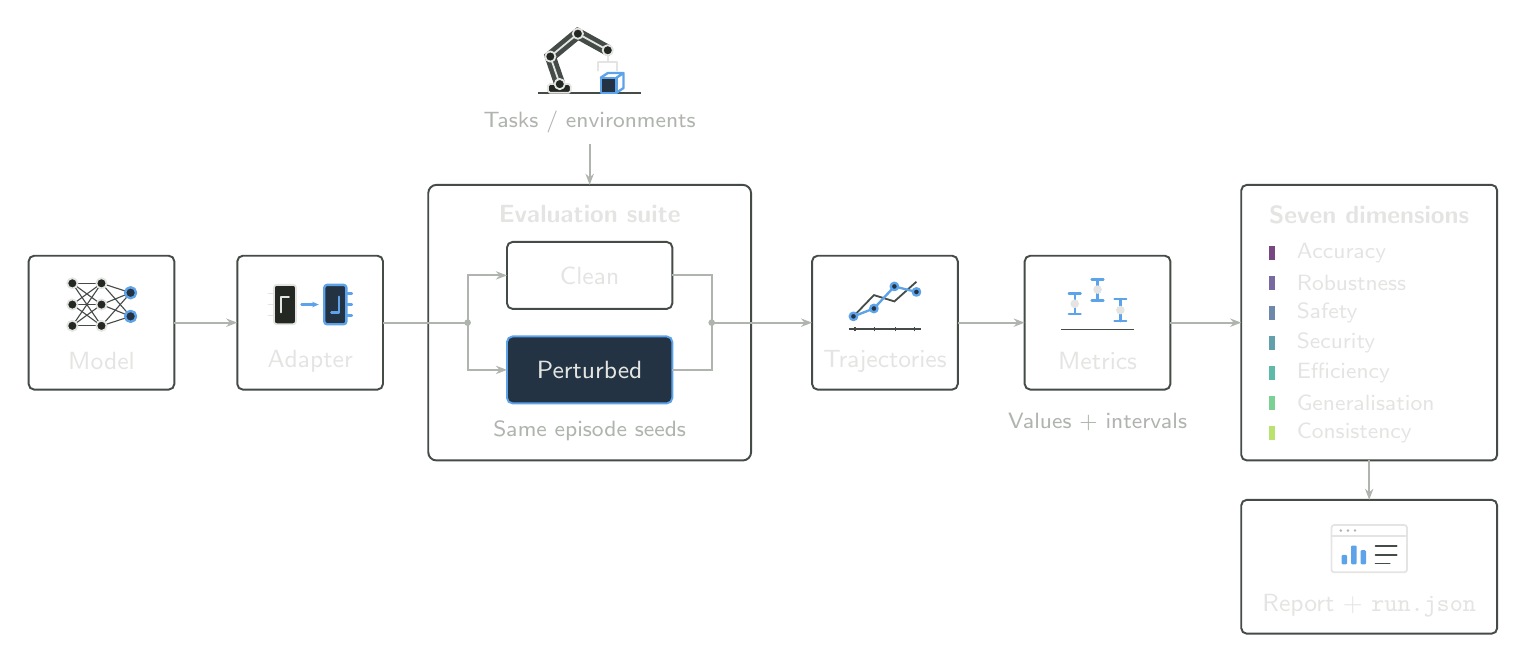
\begin{tikzpicture}[
  x=1cm,y=1cm,
  every node/.style={font=\sffamily\fontsize{9}{11}\selectfont,
    text=ink,inner sep=4pt,outer sep=0pt,align=center},
  box/.style={draw=rule,line width=0.7pt,rounded corners=2pt,
    minimum height=0.85cm,minimum width=1.85cm},
  note/.style={text=muted,font=\sffamily\fontsize{8}{10}\selectfont},
  flow/.style={draw=muted,line width=0.7pt,-{Stealth[length=4pt,width=3pt]}},
  wire/.style={draw=muted,line width=0.7pt},
  icon/.style={draw=ink,line width=0.65pt,line cap=round,line join=round},
  accenticon/.style={draw=signal,line width=0.85pt,line cap=round,line join=round},
  % Small vector illustrations share a two-tone palette and a 0.9 cm footprint.
  pics/model/.style={code={
    \foreach \a in {-0.27,0,0.27} {
      \foreach \b in {-0.27,0,0.27}
        \draw[draw=rule,line width=0.4pt] (-0.37,\a) -- (0,\b);
      \foreach \b in {-0.15,0.15}
        \draw[draw=rule,line width=0.4pt] (0,\a) -- (0.37,\b);
    }
    \foreach \x in {-0.37,0} {
      \foreach \y in {-0.27,0,0.27}
        \draw[icon,fill=panel] (\x,\y) circle (0.065);
    }
    \foreach \y in {-0.15,0.15}
      \draw[accenticon,fill=tint] (0.37,\y) circle (0.07);
  }},
  pics/adapter/.style={code={
    \draw[icon,fill=panel,rounded corners=1pt] (-0.46,-0.25) rectangle (-0.18,0.25);
    \draw[accenticon,fill=tint,rounded corners=1pt] (0.18,-0.25) rectangle (0.46,0.25);
    \foreach \y in {-0.14,0,0.14} {
      \draw[icon] (-0.53,\y) -- (-0.46,\y);
      \draw[accenticon] (0.46,\y) -- (0.53,\y);
    }
    \draw[accenticon,-{Stealth[length=2.4pt,width=2pt]}] (-0.11,0) -- (0.11,0);
    \draw[icon] (-0.37,-0.10) -- (-0.37,0.10) -- (-0.27,0.10);
    \draw[accenticon] (0.27,-0.10) -- (0.37,-0.10) -- (0.37,0.10);
  }},
  pics/trajectory/.style={code={
    \draw[draw=rule,line width=0.45pt] (-0.46,-0.31) -- (0.46,-0.31);
    \foreach \x in {-0.38,-0.13,0.13,0.38}
      \draw[draw=rule,line width=0.45pt] (\x,-0.34) -- (\x,-0.28);
    \draw[draw=rule,line width=0.65pt] (-0.40,-0.15) -- (-0.14,0.12) -- (0.12,0.04) -- (0.40,0.29);
    \draw[accenticon] (-0.40,-0.15) -- (-0.14,-0.05) -- (0.12,0.23) -- (0.40,0.16);
    \foreach \x/\y in {-0.40/-0.15,-0.14/-0.05,0.12/0.23,0.40/0.16}
      \draw[accenticon,fill=tint] (\x,\y) circle (0.047);
  }},
  pics/metrics/.style={code={
    \draw[draw=rule,line width=0.45pt] (-0.46,-0.32) -- (0.46,-0.32);
    \foreach \x/\y/\lo/\hi in {-0.29/0.01/-0.12/0.14,0/0.19/0.05/0.32,0.29/-0.07/-0.21/0.07} {
      \draw[accenticon] (\x,\lo) -- (\x,\hi)
        (\x-0.075,\lo) -- (\x+0.075,\lo)
        (\x-0.075,\hi) -- (\x+0.075,\hi);
      \fill[ink] (\x,\y) circle (0.055);
    }
  }},
  pics/scene/.style={code={
    % Articulated manipulator and an object on its work surface.
    \draw[draw=rule,line width=0.6pt] (-0.65,-0.38) -- (0.65,-0.38);
    \draw[icon,fill=panel,rounded corners=0.7pt] (-0.53,-0.38) rectangle (-0.24,-0.27);
    \draw[draw=rule,line width=4pt,line cap=round] (-0.38,-0.27) -- (-0.50,0.08) -- (-0.15,0.37) -- (0.23,0.16);
    \draw[icon] (-0.38,-0.27) -- (-0.50,0.08) -- (-0.15,0.37) -- (0.23,0.16);
    \foreach \x/\y in {-0.38/-0.27,-0.50/0.08,-0.15/0.37,0.23/0.16}
      \draw[icon,fill=panel] (\x,\y) circle (0.065);
    \draw[icon] (0.23,0.09) -- (0.23,0.01)
      (0.11,-0.10) -- (0.11,0.01) -- (0.35,0.01) -- (0.35,-0.10);
    \draw[accenticon,fill=tint] (0.14,-0.38) rectangle (0.34,-0.19);
    \draw[accenticon] (0.14,-0.19) -- (0.23,-0.13) -- (0.43,-0.13)
      -- (0.34,-0.19) (0.43,-0.13) -- (0.43,-0.32) -- (0.34,-0.38);
  }},
  pics/report/.style={code={
    \draw[icon,rounded corners=1pt] (-0.48,-0.30) rectangle (0.48,0.30);
    \draw[icon] (-0.48,0.16) -- (0.48,0.16);
    \foreach \x in {-0.36,-0.27,-0.18}
      \fill[muted] (\x,0.23) circle (0.018);
    \foreach \x/\h in {-0.35/0.12,-0.23/0.24,-0.11/0.18}
      \fill[signal,rounded corners=0.4pt] (\x,-0.20) rectangle ++(0.07,\h);
    \draw[draw=rule,line width=0.6pt,line cap=round]
      (0.08,0.03) -- (0.35,0.03) (0.08,-0.08) -- (0.35,-0.08)
      (0.08,-0.19) -- (0.26,-0.19);
  }},
]
% The suite branches into matched conditions, whose recorded trajectories feed
% the same metrics. Boxes denote operations or data, never illustrative scores.
\node[box,minimum height=1.70cm] (model) at (0,0) {};
\pic at (0,0.23) {model};
\node at (0,-0.49) {Model};
\node[box,minimum height=1.70cm] (adapter) at (2.65,0) {};
\pic at (2.65,0.23) {adapter};
\node at (2.65,-0.49) {Adapter};
\draw[flow] (model) -- (adapter);

\draw[draw=rule,line width=0.7pt,rounded corners=3pt]
  (4.15,-1.75) rectangle (8.25,1.75);
\node[font=\sffamily\bfseries\fontsize{9}{11}\selectfont]
  at (6.20,1.38) {Evaluation suite};
\node[box,minimum width=2.1cm] (clean) at (6.20,0.60) {Clean};
\node[box,minimum width=2.1cm,draw=signal,fill=tint]
  (perturbed) at (6.20,-0.60) {Perturbed};
\node[note] at (6.20,-1.38) {Same episode seeds};
\coordinate (split) at (4.65,0);
\draw[wire] (adapter.east) -- (split);
\draw[flow] (split) |- (clean.west);
\draw[flow] (split) |- (perturbed.west);
\fill[muted] (split) circle (1.2pt);

\pic at (6.20,3.30) {scene};
\node[note] (tasks) at (6.20,2.55) {Tasks / environments};
\draw[flow] (tasks.south) -- (6.20,1.75);

\node[box,minimum height=1.70cm] (trajectories) at (9.95,0) {};
\pic at (9.95,0.23) {trajectory};
\node at (9.95,-0.49) {Trajectories};
\coordinate (join) at (7.75,0);
\draw[wire] (clean.east) -| (join);
\draw[wire] (perturbed.east) -| (join);
\draw[flow] (join) -- (trajectories.west);
\fill[muted] (join) circle (1.2pt);
\node[box,minimum height=1.70cm] (metrics) at (12.65,0) {};
\pic at (12.65,0.23) {metrics};
\node at (12.65,-0.49) {Metrics};
\draw[flow] (trajectories) -- (metrics);
\node[note,anchor=north] at (12.65,-1.01) {Values + intervals};

% A compact, named output vector avoids fabricating a chart of model scores.
\node[box,minimum width=3.25cm,minimum height=3.50cm]
  (profile) at (16.10,0) {};
\node[font=\sffamily\bfseries\fontsize{9}{11}\selectfont]
  at (16.10,1.37) {Seven dimensions};
\foreach \y/\col/\title in {
  0.88/dimA/Accuracy,
  0.50/dimB/Robustness,
  0.12/dimC/Safety,
  -0.26/dimD/Security,
  -0.64/dimE/Efficiency,
  -1.02/dimF/Generalisation,
  -1.40/dimG/Consistency} {
  \fill[\col] (14.83,\y-0.09) rectangle ++(0.07,0.18);
  \node[anchor=west,font=\sffamily\fontsize{8.5}{10}\selectfont]
    at (15.04,\y) {\title};
}
\draw[flow] (metrics) -- (profile);
\node[box,minimum width=3.25cm,minimum height=1.70cm] (artifacts) at (16.10,-3.10) {};
\pic at (16.10,-2.87) {report};
\node at (16.10,-3.59) {Report + \texttt{run.json}};
\draw[flow] (profile) -- (artifacts);
\end{tikzpicture}
\end{document}
"
%   pdflatex -jobname=method-dark  "\def\xevalstheme{dark}% Documentation method diagram. Build both themes with TeX Live and poppler:
%   pdflatex -jobname=method-light "\def\xevalstheme{light}% Documentation method diagram. Build both themes with TeX Live and poppler:
%   pdflatex -jobname=method-light "\def\xevalstheme{light}\input{method.tex}"
%   pdflatex -jobname=method-dark  "\def\xevalstheme{dark}\input{method.tex}"
%   pdftocairo -svg method-light.pdf method-light.svg
%   pdftocairo -svg method-dark.pdf method-dark.svg
% Commit the SVGs; documentation builds do not require LaTeX.
\documentclass[border=8pt]{standalone}
\usepackage[T1]{fontenc}
\usepackage{lmodern}
\usepackage{xcolor}
\usepackage{tikz}
\usetikzlibrary{arrows.meta}
\providecommand{\xevalstheme}{light}
\def\xevalslight{light}
\ifx\xevalstheme\xevalslight
  \definecolor{ink}{HTML}{121412}
  \definecolor{muted}{HTML}{5C615D}
  \definecolor{rule}{HTML}{A8ADA7}
  \definecolor{panel}{HTML}{F1F2EF}
  \definecolor{signal}{HTML}{367FC9}
  \definecolor{tint}{HTML}{E8F0F8}
  \definecolor{dimA}{HTML}{440154}\definecolor{dimB}{HTML}{46327E}
  \definecolor{dimC}{HTML}{365C8D}\definecolor{dimD}{HTML}{277F8E}
  \definecolor{dimE}{HTML}{1FA187}\definecolor{dimF}{HTML}{4AC16D}
  \definecolor{dimG}{HTML}{A0DA39}
\else
  \definecolor{ink}{HTML}{E4E5E2}
  \definecolor{muted}{HTML}{AFB4AE}
  \definecolor{rule}{HTML}{454B46}
  \definecolor{panel}{HTML}{232823}
  \definecolor{signal}{HTML}{5DA3E9}
  \definecolor{tint}{HTML}{233344}
  \definecolor{dimA}{HTML}{774782}\definecolor{dimB}{HTML}{786AA0}
  \definecolor{dimC}{HTML}{6D88AB}\definecolor{dimD}{HTML}{62A1AC}
  \definecolor{dimE}{HTML}{5CBAA7}\definecolor{dimF}{HTML}{7BD194}
  \definecolor{dimG}{HTML}{B9E36E}
\fi
\begin{document}
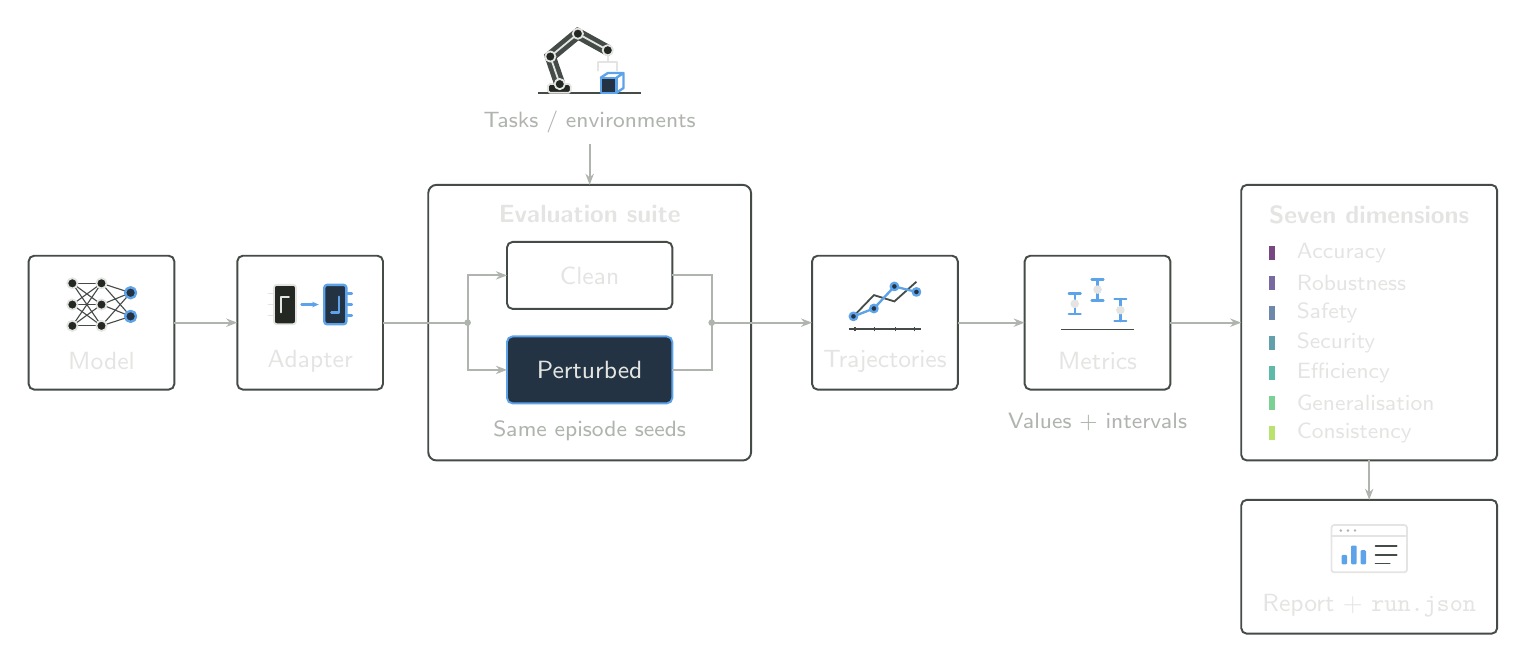
\begin{tikzpicture}[
  x=1cm,y=1cm,
  every node/.style={font=\sffamily\fontsize{9}{11}\selectfont,
    text=ink,inner sep=4pt,outer sep=0pt,align=center},
  box/.style={draw=rule,line width=0.7pt,rounded corners=2pt,
    minimum height=0.85cm,minimum width=1.85cm},
  note/.style={text=muted,font=\sffamily\fontsize{8}{10}\selectfont},
  flow/.style={draw=muted,line width=0.7pt,-{Stealth[length=4pt,width=3pt]}},
  wire/.style={draw=muted,line width=0.7pt},
  icon/.style={draw=ink,line width=0.65pt,line cap=round,line join=round},
  accenticon/.style={draw=signal,line width=0.85pt,line cap=round,line join=round},
  % Small vector illustrations share a two-tone palette and a 0.9 cm footprint.
  pics/model/.style={code={
    \foreach \a in {-0.27,0,0.27} {
      \foreach \b in {-0.27,0,0.27}
        \draw[draw=rule,line width=0.4pt] (-0.37,\a) -- (0,\b);
      \foreach \b in {-0.15,0.15}
        \draw[draw=rule,line width=0.4pt] (0,\a) -- (0.37,\b);
    }
    \foreach \x in {-0.37,0} {
      \foreach \y in {-0.27,0,0.27}
        \draw[icon,fill=panel] (\x,\y) circle (0.065);
    }
    \foreach \y in {-0.15,0.15}
      \draw[accenticon,fill=tint] (0.37,\y) circle (0.07);
  }},
  pics/adapter/.style={code={
    \draw[icon,fill=panel,rounded corners=1pt] (-0.46,-0.25) rectangle (-0.18,0.25);
    \draw[accenticon,fill=tint,rounded corners=1pt] (0.18,-0.25) rectangle (0.46,0.25);
    \foreach \y in {-0.14,0,0.14} {
      \draw[icon] (-0.53,\y) -- (-0.46,\y);
      \draw[accenticon] (0.46,\y) -- (0.53,\y);
    }
    \draw[accenticon,-{Stealth[length=2.4pt,width=2pt]}] (-0.11,0) -- (0.11,0);
    \draw[icon] (-0.37,-0.10) -- (-0.37,0.10) -- (-0.27,0.10);
    \draw[accenticon] (0.27,-0.10) -- (0.37,-0.10) -- (0.37,0.10);
  }},
  pics/trajectory/.style={code={
    \draw[draw=rule,line width=0.45pt] (-0.46,-0.31) -- (0.46,-0.31);
    \foreach \x in {-0.38,-0.13,0.13,0.38}
      \draw[draw=rule,line width=0.45pt] (\x,-0.34) -- (\x,-0.28);
    \draw[draw=rule,line width=0.65pt] (-0.40,-0.15) -- (-0.14,0.12) -- (0.12,0.04) -- (0.40,0.29);
    \draw[accenticon] (-0.40,-0.15) -- (-0.14,-0.05) -- (0.12,0.23) -- (0.40,0.16);
    \foreach \x/\y in {-0.40/-0.15,-0.14/-0.05,0.12/0.23,0.40/0.16}
      \draw[accenticon,fill=tint] (\x,\y) circle (0.047);
  }},
  pics/metrics/.style={code={
    \draw[draw=rule,line width=0.45pt] (-0.46,-0.32) -- (0.46,-0.32);
    \foreach \x/\y/\lo/\hi in {-0.29/0.01/-0.12/0.14,0/0.19/0.05/0.32,0.29/-0.07/-0.21/0.07} {
      \draw[accenticon] (\x,\lo) -- (\x,\hi)
        (\x-0.075,\lo) -- (\x+0.075,\lo)
        (\x-0.075,\hi) -- (\x+0.075,\hi);
      \fill[ink] (\x,\y) circle (0.055);
    }
  }},
  pics/scene/.style={code={
    % Articulated manipulator and an object on its work surface.
    \draw[draw=rule,line width=0.6pt] (-0.65,-0.38) -- (0.65,-0.38);
    \draw[icon,fill=panel,rounded corners=0.7pt] (-0.53,-0.38) rectangle (-0.24,-0.27);
    \draw[draw=rule,line width=4pt,line cap=round] (-0.38,-0.27) -- (-0.50,0.08) -- (-0.15,0.37) -- (0.23,0.16);
    \draw[icon] (-0.38,-0.27) -- (-0.50,0.08) -- (-0.15,0.37) -- (0.23,0.16);
    \foreach \x/\y in {-0.38/-0.27,-0.50/0.08,-0.15/0.37,0.23/0.16}
      \draw[icon,fill=panel] (\x,\y) circle (0.065);
    \draw[icon] (0.23,0.09) -- (0.23,0.01)
      (0.11,-0.10) -- (0.11,0.01) -- (0.35,0.01) -- (0.35,-0.10);
    \draw[accenticon,fill=tint] (0.14,-0.38) rectangle (0.34,-0.19);
    \draw[accenticon] (0.14,-0.19) -- (0.23,-0.13) -- (0.43,-0.13)
      -- (0.34,-0.19) (0.43,-0.13) -- (0.43,-0.32) -- (0.34,-0.38);
  }},
  pics/report/.style={code={
    \draw[icon,rounded corners=1pt] (-0.48,-0.30) rectangle (0.48,0.30);
    \draw[icon] (-0.48,0.16) -- (0.48,0.16);
    \foreach \x in {-0.36,-0.27,-0.18}
      \fill[muted] (\x,0.23) circle (0.018);
    \foreach \x/\h in {-0.35/0.12,-0.23/0.24,-0.11/0.18}
      \fill[signal,rounded corners=0.4pt] (\x,-0.20) rectangle ++(0.07,\h);
    \draw[draw=rule,line width=0.6pt,line cap=round]
      (0.08,0.03) -- (0.35,0.03) (0.08,-0.08) -- (0.35,-0.08)
      (0.08,-0.19) -- (0.26,-0.19);
  }},
]
% The suite branches into matched conditions, whose recorded trajectories feed
% the same metrics. Boxes denote operations or data, never illustrative scores.
\node[box,minimum height=1.70cm] (model) at (0,0) {};
\pic at (0,0.23) {model};
\node at (0,-0.49) {Model};
\node[box,minimum height=1.70cm] (adapter) at (2.65,0) {};
\pic at (2.65,0.23) {adapter};
\node at (2.65,-0.49) {Adapter};
\draw[flow] (model) -- (adapter);

\draw[draw=rule,line width=0.7pt,rounded corners=3pt]
  (4.15,-1.75) rectangle (8.25,1.75);
\node[font=\sffamily\bfseries\fontsize{9}{11}\selectfont]
  at (6.20,1.38) {Evaluation suite};
\node[box,minimum width=2.1cm] (clean) at (6.20,0.60) {Clean};
\node[box,minimum width=2.1cm,draw=signal,fill=tint]
  (perturbed) at (6.20,-0.60) {Perturbed};
\node[note] at (6.20,-1.38) {Same episode seeds};
\coordinate (split) at (4.65,0);
\draw[wire] (adapter.east) -- (split);
\draw[flow] (split) |- (clean.west);
\draw[flow] (split) |- (perturbed.west);
\fill[muted] (split) circle (1.2pt);

\pic at (6.20,3.30) {scene};
\node[note] (tasks) at (6.20,2.55) {Tasks / environments};
\draw[flow] (tasks.south) -- (6.20,1.75);

\node[box,minimum height=1.70cm] (trajectories) at (9.95,0) {};
\pic at (9.95,0.23) {trajectory};
\node at (9.95,-0.49) {Trajectories};
\coordinate (join) at (7.75,0);
\draw[wire] (clean.east) -| (join);
\draw[wire] (perturbed.east) -| (join);
\draw[flow] (join) -- (trajectories.west);
\fill[muted] (join) circle (1.2pt);
\node[box,minimum height=1.70cm] (metrics) at (12.65,0) {};
\pic at (12.65,0.23) {metrics};
\node at (12.65,-0.49) {Metrics};
\draw[flow] (trajectories) -- (metrics);
\node[note,anchor=north] at (12.65,-1.01) {Values + intervals};

% A compact, named output vector avoids fabricating a chart of model scores.
\node[box,minimum width=3.25cm,minimum height=3.50cm]
  (profile) at (16.10,0) {};
\node[font=\sffamily\bfseries\fontsize{9}{11}\selectfont]
  at (16.10,1.37) {Seven dimensions};
\foreach \y/\col/\title in {
  0.88/dimA/Accuracy,
  0.50/dimB/Robustness,
  0.12/dimC/Safety,
  -0.26/dimD/Security,
  -0.64/dimE/Efficiency,
  -1.02/dimF/Generalisation,
  -1.40/dimG/Consistency} {
  \fill[\col] (14.83,\y-0.09) rectangle ++(0.07,0.18);
  \node[anchor=west,font=\sffamily\fontsize{8.5}{10}\selectfont]
    at (15.04,\y) {\title};
}
\draw[flow] (metrics) -- (profile);
\node[box,minimum width=3.25cm,minimum height=1.70cm] (artifacts) at (16.10,-3.10) {};
\pic at (16.10,-2.87) {report};
\node at (16.10,-3.59) {Report + \texttt{run.json}};
\draw[flow] (profile) -- (artifacts);
\end{tikzpicture}
\end{document}
"
%   pdflatex -jobname=method-dark  "\def\xevalstheme{dark}% Documentation method diagram. Build both themes with TeX Live and poppler:
%   pdflatex -jobname=method-light "\def\xevalstheme{light}\input{method.tex}"
%   pdflatex -jobname=method-dark  "\def\xevalstheme{dark}\input{method.tex}"
%   pdftocairo -svg method-light.pdf method-light.svg
%   pdftocairo -svg method-dark.pdf method-dark.svg
% Commit the SVGs; documentation builds do not require LaTeX.
\documentclass[border=8pt]{standalone}
\usepackage[T1]{fontenc}
\usepackage{lmodern}
\usepackage{xcolor}
\usepackage{tikz}
\usetikzlibrary{arrows.meta}
\providecommand{\xevalstheme}{light}
\def\xevalslight{light}
\ifx\xevalstheme\xevalslight
  \definecolor{ink}{HTML}{121412}
  \definecolor{muted}{HTML}{5C615D}
  \definecolor{rule}{HTML}{A8ADA7}
  \definecolor{panel}{HTML}{F1F2EF}
  \definecolor{signal}{HTML}{367FC9}
  \definecolor{tint}{HTML}{E8F0F8}
  \definecolor{dimA}{HTML}{440154}\definecolor{dimB}{HTML}{46327E}
  \definecolor{dimC}{HTML}{365C8D}\definecolor{dimD}{HTML}{277F8E}
  \definecolor{dimE}{HTML}{1FA187}\definecolor{dimF}{HTML}{4AC16D}
  \definecolor{dimG}{HTML}{A0DA39}
\else
  \definecolor{ink}{HTML}{E4E5E2}
  \definecolor{muted}{HTML}{AFB4AE}
  \definecolor{rule}{HTML}{454B46}
  \definecolor{panel}{HTML}{232823}
  \definecolor{signal}{HTML}{5DA3E9}
  \definecolor{tint}{HTML}{233344}
  \definecolor{dimA}{HTML}{774782}\definecolor{dimB}{HTML}{786AA0}
  \definecolor{dimC}{HTML}{6D88AB}\definecolor{dimD}{HTML}{62A1AC}
  \definecolor{dimE}{HTML}{5CBAA7}\definecolor{dimF}{HTML}{7BD194}
  \definecolor{dimG}{HTML}{B9E36E}
\fi
\begin{document}
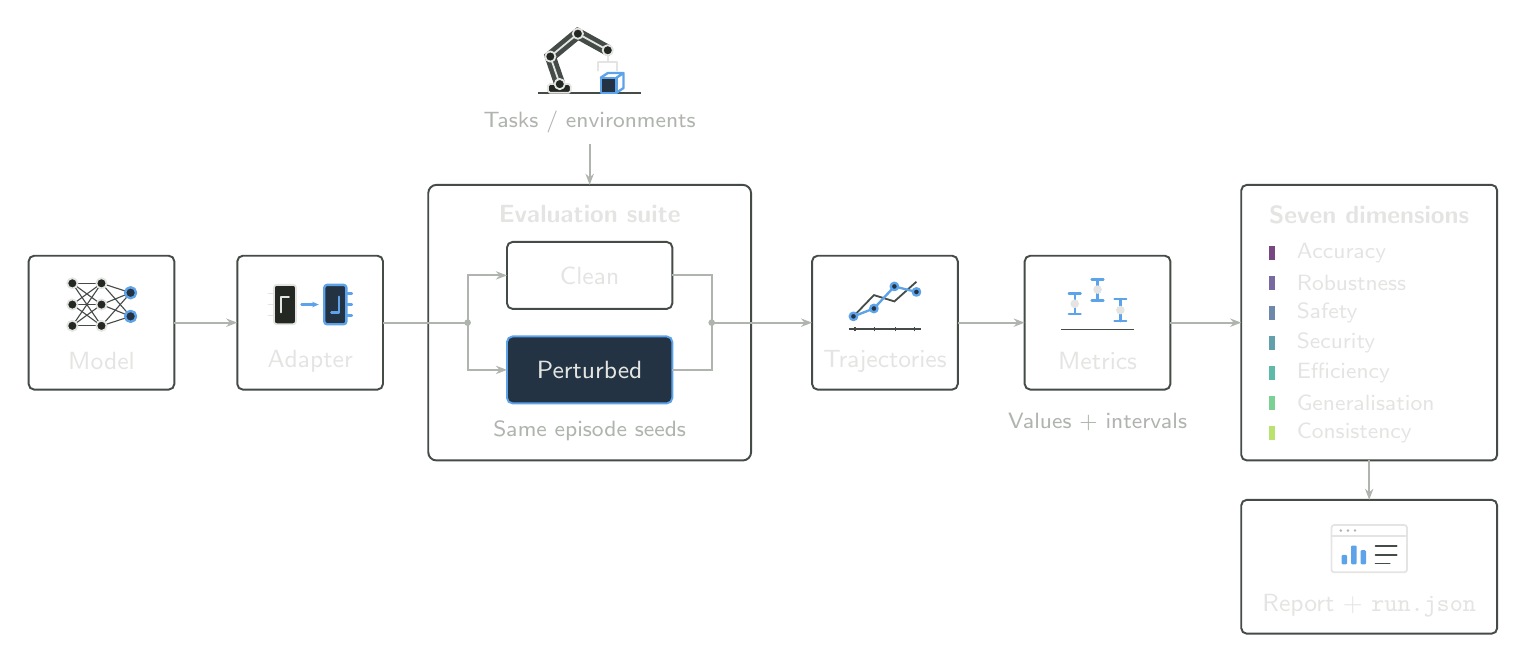
\begin{tikzpicture}[
  x=1cm,y=1cm,
  every node/.style={font=\sffamily\fontsize{9}{11}\selectfont,
    text=ink,inner sep=4pt,outer sep=0pt,align=center},
  box/.style={draw=rule,line width=0.7pt,rounded corners=2pt,
    minimum height=0.85cm,minimum width=1.85cm},
  note/.style={text=muted,font=\sffamily\fontsize{8}{10}\selectfont},
  flow/.style={draw=muted,line width=0.7pt,-{Stealth[length=4pt,width=3pt]}},
  wire/.style={draw=muted,line width=0.7pt},
  icon/.style={draw=ink,line width=0.65pt,line cap=round,line join=round},
  accenticon/.style={draw=signal,line width=0.85pt,line cap=round,line join=round},
  % Small vector illustrations share a two-tone palette and a 0.9 cm footprint.
  pics/model/.style={code={
    \foreach \a in {-0.27,0,0.27} {
      \foreach \b in {-0.27,0,0.27}
        \draw[draw=rule,line width=0.4pt] (-0.37,\a) -- (0,\b);
      \foreach \b in {-0.15,0.15}
        \draw[draw=rule,line width=0.4pt] (0,\a) -- (0.37,\b);
    }
    \foreach \x in {-0.37,0} {
      \foreach \y in {-0.27,0,0.27}
        \draw[icon,fill=panel] (\x,\y) circle (0.065);
    }
    \foreach \y in {-0.15,0.15}
      \draw[accenticon,fill=tint] (0.37,\y) circle (0.07);
  }},
  pics/adapter/.style={code={
    \draw[icon,fill=panel,rounded corners=1pt] (-0.46,-0.25) rectangle (-0.18,0.25);
    \draw[accenticon,fill=tint,rounded corners=1pt] (0.18,-0.25) rectangle (0.46,0.25);
    \foreach \y in {-0.14,0,0.14} {
      \draw[icon] (-0.53,\y) -- (-0.46,\y);
      \draw[accenticon] (0.46,\y) -- (0.53,\y);
    }
    \draw[accenticon,-{Stealth[length=2.4pt,width=2pt]}] (-0.11,0) -- (0.11,0);
    \draw[icon] (-0.37,-0.10) -- (-0.37,0.10) -- (-0.27,0.10);
    \draw[accenticon] (0.27,-0.10) -- (0.37,-0.10) -- (0.37,0.10);
  }},
  pics/trajectory/.style={code={
    \draw[draw=rule,line width=0.45pt] (-0.46,-0.31) -- (0.46,-0.31);
    \foreach \x in {-0.38,-0.13,0.13,0.38}
      \draw[draw=rule,line width=0.45pt] (\x,-0.34) -- (\x,-0.28);
    \draw[draw=rule,line width=0.65pt] (-0.40,-0.15) -- (-0.14,0.12) -- (0.12,0.04) -- (0.40,0.29);
    \draw[accenticon] (-0.40,-0.15) -- (-0.14,-0.05) -- (0.12,0.23) -- (0.40,0.16);
    \foreach \x/\y in {-0.40/-0.15,-0.14/-0.05,0.12/0.23,0.40/0.16}
      \draw[accenticon,fill=tint] (\x,\y) circle (0.047);
  }},
  pics/metrics/.style={code={
    \draw[draw=rule,line width=0.45pt] (-0.46,-0.32) -- (0.46,-0.32);
    \foreach \x/\y/\lo/\hi in {-0.29/0.01/-0.12/0.14,0/0.19/0.05/0.32,0.29/-0.07/-0.21/0.07} {
      \draw[accenticon] (\x,\lo) -- (\x,\hi)
        (\x-0.075,\lo) -- (\x+0.075,\lo)
        (\x-0.075,\hi) -- (\x+0.075,\hi);
      \fill[ink] (\x,\y) circle (0.055);
    }
  }},
  pics/scene/.style={code={
    % Articulated manipulator and an object on its work surface.
    \draw[draw=rule,line width=0.6pt] (-0.65,-0.38) -- (0.65,-0.38);
    \draw[icon,fill=panel,rounded corners=0.7pt] (-0.53,-0.38) rectangle (-0.24,-0.27);
    \draw[draw=rule,line width=4pt,line cap=round] (-0.38,-0.27) -- (-0.50,0.08) -- (-0.15,0.37) -- (0.23,0.16);
    \draw[icon] (-0.38,-0.27) -- (-0.50,0.08) -- (-0.15,0.37) -- (0.23,0.16);
    \foreach \x/\y in {-0.38/-0.27,-0.50/0.08,-0.15/0.37,0.23/0.16}
      \draw[icon,fill=panel] (\x,\y) circle (0.065);
    \draw[icon] (0.23,0.09) -- (0.23,0.01)
      (0.11,-0.10) -- (0.11,0.01) -- (0.35,0.01) -- (0.35,-0.10);
    \draw[accenticon,fill=tint] (0.14,-0.38) rectangle (0.34,-0.19);
    \draw[accenticon] (0.14,-0.19) -- (0.23,-0.13) -- (0.43,-0.13)
      -- (0.34,-0.19) (0.43,-0.13) -- (0.43,-0.32) -- (0.34,-0.38);
  }},
  pics/report/.style={code={
    \draw[icon,rounded corners=1pt] (-0.48,-0.30) rectangle (0.48,0.30);
    \draw[icon] (-0.48,0.16) -- (0.48,0.16);
    \foreach \x in {-0.36,-0.27,-0.18}
      \fill[muted] (\x,0.23) circle (0.018);
    \foreach \x/\h in {-0.35/0.12,-0.23/0.24,-0.11/0.18}
      \fill[signal,rounded corners=0.4pt] (\x,-0.20) rectangle ++(0.07,\h);
    \draw[draw=rule,line width=0.6pt,line cap=round]
      (0.08,0.03) -- (0.35,0.03) (0.08,-0.08) -- (0.35,-0.08)
      (0.08,-0.19) -- (0.26,-0.19);
  }},
]
% The suite branches into matched conditions, whose recorded trajectories feed
% the same metrics. Boxes denote operations or data, never illustrative scores.
\node[box,minimum height=1.70cm] (model) at (0,0) {};
\pic at (0,0.23) {model};
\node at (0,-0.49) {Model};
\node[box,minimum height=1.70cm] (adapter) at (2.65,0) {};
\pic at (2.65,0.23) {adapter};
\node at (2.65,-0.49) {Adapter};
\draw[flow] (model) -- (adapter);

\draw[draw=rule,line width=0.7pt,rounded corners=3pt]
  (4.15,-1.75) rectangle (8.25,1.75);
\node[font=\sffamily\bfseries\fontsize{9}{11}\selectfont]
  at (6.20,1.38) {Evaluation suite};
\node[box,minimum width=2.1cm] (clean) at (6.20,0.60) {Clean};
\node[box,minimum width=2.1cm,draw=signal,fill=tint]
  (perturbed) at (6.20,-0.60) {Perturbed};
\node[note] at (6.20,-1.38) {Same episode seeds};
\coordinate (split) at (4.65,0);
\draw[wire] (adapter.east) -- (split);
\draw[flow] (split) |- (clean.west);
\draw[flow] (split) |- (perturbed.west);
\fill[muted] (split) circle (1.2pt);

\pic at (6.20,3.30) {scene};
\node[note] (tasks) at (6.20,2.55) {Tasks / environments};
\draw[flow] (tasks.south) -- (6.20,1.75);

\node[box,minimum height=1.70cm] (trajectories) at (9.95,0) {};
\pic at (9.95,0.23) {trajectory};
\node at (9.95,-0.49) {Trajectories};
\coordinate (join) at (7.75,0);
\draw[wire] (clean.east) -| (join);
\draw[wire] (perturbed.east) -| (join);
\draw[flow] (join) -- (trajectories.west);
\fill[muted] (join) circle (1.2pt);
\node[box,minimum height=1.70cm] (metrics) at (12.65,0) {};
\pic at (12.65,0.23) {metrics};
\node at (12.65,-0.49) {Metrics};
\draw[flow] (trajectories) -- (metrics);
\node[note,anchor=north] at (12.65,-1.01) {Values + intervals};

% A compact, named output vector avoids fabricating a chart of model scores.
\node[box,minimum width=3.25cm,minimum height=3.50cm]
  (profile) at (16.10,0) {};
\node[font=\sffamily\bfseries\fontsize{9}{11}\selectfont]
  at (16.10,1.37) {Seven dimensions};
\foreach \y/\col/\title in {
  0.88/dimA/Accuracy,
  0.50/dimB/Robustness,
  0.12/dimC/Safety,
  -0.26/dimD/Security,
  -0.64/dimE/Efficiency,
  -1.02/dimF/Generalisation,
  -1.40/dimG/Consistency} {
  \fill[\col] (14.83,\y-0.09) rectangle ++(0.07,0.18);
  \node[anchor=west,font=\sffamily\fontsize{8.5}{10}\selectfont]
    at (15.04,\y) {\title};
}
\draw[flow] (metrics) -- (profile);
\node[box,minimum width=3.25cm,minimum height=1.70cm] (artifacts) at (16.10,-3.10) {};
\pic at (16.10,-2.87) {report};
\node at (16.10,-3.59) {Report + \texttt{run.json}};
\draw[flow] (profile) -- (artifacts);
\end{tikzpicture}
\end{document}
"
%   pdftocairo -svg method-light.pdf method-light.svg
%   pdftocairo -svg method-dark.pdf method-dark.svg
% Commit the SVGs; documentation builds do not require LaTeX.
\documentclass[border=8pt]{standalone}
\usepackage[T1]{fontenc}
\usepackage{lmodern}
\usepackage{xcolor}
\usepackage{tikz}
\usetikzlibrary{arrows.meta}
\providecommand{\xevalstheme}{light}
\def\xevalslight{light}
\ifx\xevalstheme\xevalslight
  \definecolor{ink}{HTML}{121412}
  \definecolor{muted}{HTML}{5C615D}
  \definecolor{rule}{HTML}{A8ADA7}
  \definecolor{panel}{HTML}{F1F2EF}
  \definecolor{signal}{HTML}{367FC9}
  \definecolor{tint}{HTML}{E8F0F8}
  \definecolor{dimA}{HTML}{440154}\definecolor{dimB}{HTML}{46327E}
  \definecolor{dimC}{HTML}{365C8D}\definecolor{dimD}{HTML}{277F8E}
  \definecolor{dimE}{HTML}{1FA187}\definecolor{dimF}{HTML}{4AC16D}
  \definecolor{dimG}{HTML}{A0DA39}
\else
  \definecolor{ink}{HTML}{E4E5E2}
  \definecolor{muted}{HTML}{AFB4AE}
  \definecolor{rule}{HTML}{454B46}
  \definecolor{panel}{HTML}{232823}
  \definecolor{signal}{HTML}{5DA3E9}
  \definecolor{tint}{HTML}{233344}
  \definecolor{dimA}{HTML}{774782}\definecolor{dimB}{HTML}{786AA0}
  \definecolor{dimC}{HTML}{6D88AB}\definecolor{dimD}{HTML}{62A1AC}
  \definecolor{dimE}{HTML}{5CBAA7}\definecolor{dimF}{HTML}{7BD194}
  \definecolor{dimG}{HTML}{B9E36E}
\fi
\begin{document}
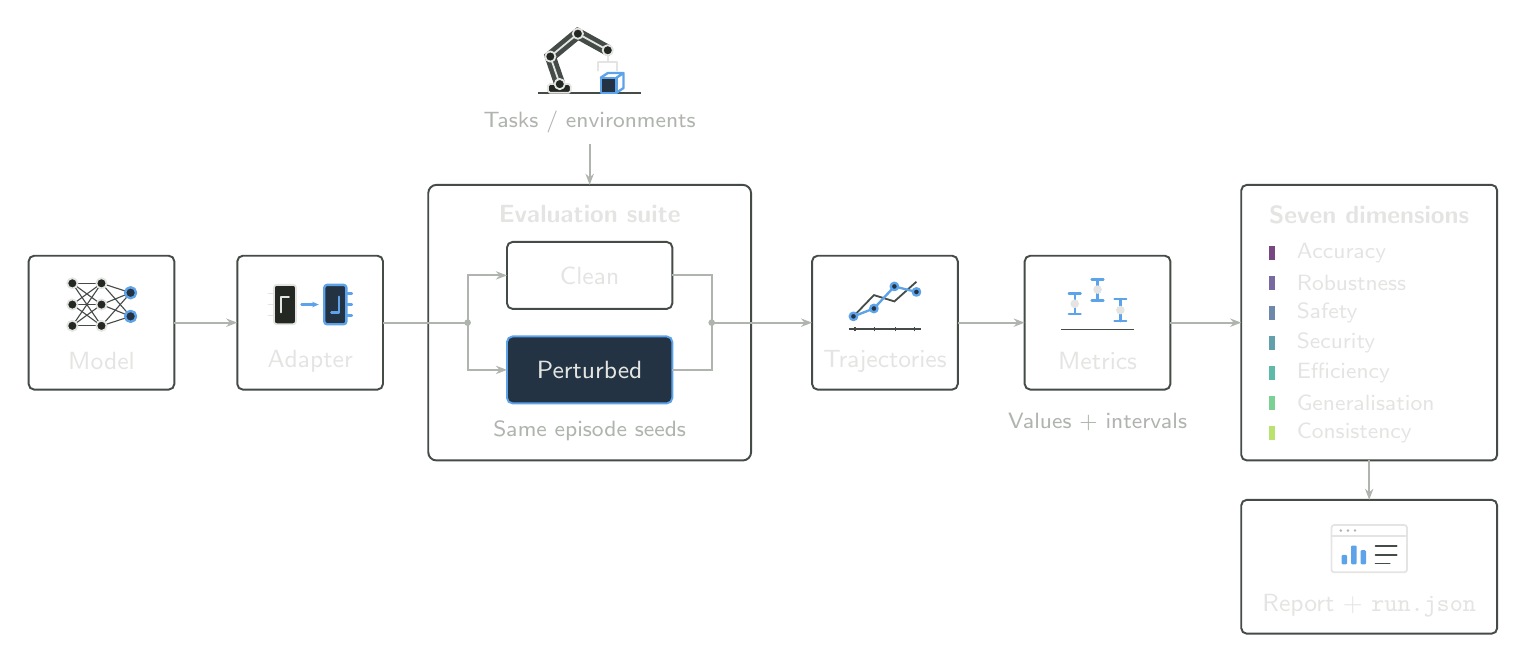
\begin{tikzpicture}[
  x=1cm,y=1cm,
  every node/.style={font=\sffamily\fontsize{9}{11}\selectfont,
    text=ink,inner sep=4pt,outer sep=0pt,align=center},
  box/.style={draw=rule,line width=0.7pt,rounded corners=2pt,
    minimum height=0.85cm,minimum width=1.85cm},
  note/.style={text=muted,font=\sffamily\fontsize{8}{10}\selectfont},
  flow/.style={draw=muted,line width=0.7pt,-{Stealth[length=4pt,width=3pt]}},
  wire/.style={draw=muted,line width=0.7pt},
  icon/.style={draw=ink,line width=0.65pt,line cap=round,line join=round},
  accenticon/.style={draw=signal,line width=0.85pt,line cap=round,line join=round},
  % Small vector illustrations share a two-tone palette and a 0.9 cm footprint.
  pics/model/.style={code={
    \foreach \a in {-0.27,0,0.27} {
      \foreach \b in {-0.27,0,0.27}
        \draw[draw=rule,line width=0.4pt] (-0.37,\a) -- (0,\b);
      \foreach \b in {-0.15,0.15}
        \draw[draw=rule,line width=0.4pt] (0,\a) -- (0.37,\b);
    }
    \foreach \x in {-0.37,0} {
      \foreach \y in {-0.27,0,0.27}
        \draw[icon,fill=panel] (\x,\y) circle (0.065);
    }
    \foreach \y in {-0.15,0.15}
      \draw[accenticon,fill=tint] (0.37,\y) circle (0.07);
  }},
  pics/adapter/.style={code={
    \draw[icon,fill=panel,rounded corners=1pt] (-0.46,-0.25) rectangle (-0.18,0.25);
    \draw[accenticon,fill=tint,rounded corners=1pt] (0.18,-0.25) rectangle (0.46,0.25);
    \foreach \y in {-0.14,0,0.14} {
      \draw[icon] (-0.53,\y) -- (-0.46,\y);
      \draw[accenticon] (0.46,\y) -- (0.53,\y);
    }
    \draw[accenticon,-{Stealth[length=2.4pt,width=2pt]}] (-0.11,0) -- (0.11,0);
    \draw[icon] (-0.37,-0.10) -- (-0.37,0.10) -- (-0.27,0.10);
    \draw[accenticon] (0.27,-0.10) -- (0.37,-0.10) -- (0.37,0.10);
  }},
  pics/trajectory/.style={code={
    \draw[draw=rule,line width=0.45pt] (-0.46,-0.31) -- (0.46,-0.31);
    \foreach \x in {-0.38,-0.13,0.13,0.38}
      \draw[draw=rule,line width=0.45pt] (\x,-0.34) -- (\x,-0.28);
    \draw[draw=rule,line width=0.65pt] (-0.40,-0.15) -- (-0.14,0.12) -- (0.12,0.04) -- (0.40,0.29);
    \draw[accenticon] (-0.40,-0.15) -- (-0.14,-0.05) -- (0.12,0.23) -- (0.40,0.16);
    \foreach \x/\y in {-0.40/-0.15,-0.14/-0.05,0.12/0.23,0.40/0.16}
      \draw[accenticon,fill=tint] (\x,\y) circle (0.047);
  }},
  pics/metrics/.style={code={
    \draw[draw=rule,line width=0.45pt] (-0.46,-0.32) -- (0.46,-0.32);
    \foreach \x/\y/\lo/\hi in {-0.29/0.01/-0.12/0.14,0/0.19/0.05/0.32,0.29/-0.07/-0.21/0.07} {
      \draw[accenticon] (\x,\lo) -- (\x,\hi)
        (\x-0.075,\lo) -- (\x+0.075,\lo)
        (\x-0.075,\hi) -- (\x+0.075,\hi);
      \fill[ink] (\x,\y) circle (0.055);
    }
  }},
  pics/scene/.style={code={
    % Articulated manipulator and an object on its work surface.
    \draw[draw=rule,line width=0.6pt] (-0.65,-0.38) -- (0.65,-0.38);
    \draw[icon,fill=panel,rounded corners=0.7pt] (-0.53,-0.38) rectangle (-0.24,-0.27);
    \draw[draw=rule,line width=4pt,line cap=round] (-0.38,-0.27) -- (-0.50,0.08) -- (-0.15,0.37) -- (0.23,0.16);
    \draw[icon] (-0.38,-0.27) -- (-0.50,0.08) -- (-0.15,0.37) -- (0.23,0.16);
    \foreach \x/\y in {-0.38/-0.27,-0.50/0.08,-0.15/0.37,0.23/0.16}
      \draw[icon,fill=panel] (\x,\y) circle (0.065);
    \draw[icon] (0.23,0.09) -- (0.23,0.01)
      (0.11,-0.10) -- (0.11,0.01) -- (0.35,0.01) -- (0.35,-0.10);
    \draw[accenticon,fill=tint] (0.14,-0.38) rectangle (0.34,-0.19);
    \draw[accenticon] (0.14,-0.19) -- (0.23,-0.13) -- (0.43,-0.13)
      -- (0.34,-0.19) (0.43,-0.13) -- (0.43,-0.32) -- (0.34,-0.38);
  }},
  pics/report/.style={code={
    \draw[icon,rounded corners=1pt] (-0.48,-0.30) rectangle (0.48,0.30);
    \draw[icon] (-0.48,0.16) -- (0.48,0.16);
    \foreach \x in {-0.36,-0.27,-0.18}
      \fill[muted] (\x,0.23) circle (0.018);
    \foreach \x/\h in {-0.35/0.12,-0.23/0.24,-0.11/0.18}
      \fill[signal,rounded corners=0.4pt] (\x,-0.20) rectangle ++(0.07,\h);
    \draw[draw=rule,line width=0.6pt,line cap=round]
      (0.08,0.03) -- (0.35,0.03) (0.08,-0.08) -- (0.35,-0.08)
      (0.08,-0.19) -- (0.26,-0.19);
  }},
]
% The suite branches into matched conditions, whose recorded trajectories feed
% the same metrics. Boxes denote operations or data, never illustrative scores.
\node[box,minimum height=1.70cm] (model) at (0,0) {};
\pic at (0,0.23) {model};
\node at (0,-0.49) {Model};
\node[box,minimum height=1.70cm] (adapter) at (2.65,0) {};
\pic at (2.65,0.23) {adapter};
\node at (2.65,-0.49) {Adapter};
\draw[flow] (model) -- (adapter);

\draw[draw=rule,line width=0.7pt,rounded corners=3pt]
  (4.15,-1.75) rectangle (8.25,1.75);
\node[font=\sffamily\bfseries\fontsize{9}{11}\selectfont]
  at (6.20,1.38) {Evaluation suite};
\node[box,minimum width=2.1cm] (clean) at (6.20,0.60) {Clean};
\node[box,minimum width=2.1cm,draw=signal,fill=tint]
  (perturbed) at (6.20,-0.60) {Perturbed};
\node[note] at (6.20,-1.38) {Same episode seeds};
\coordinate (split) at (4.65,0);
\draw[wire] (adapter.east) -- (split);
\draw[flow] (split) |- (clean.west);
\draw[flow] (split) |- (perturbed.west);
\fill[muted] (split) circle (1.2pt);

\pic at (6.20,3.30) {scene};
\node[note] (tasks) at (6.20,2.55) {Tasks / environments};
\draw[flow] (tasks.south) -- (6.20,1.75);

\node[box,minimum height=1.70cm] (trajectories) at (9.95,0) {};
\pic at (9.95,0.23) {trajectory};
\node at (9.95,-0.49) {Trajectories};
\coordinate (join) at (7.75,0);
\draw[wire] (clean.east) -| (join);
\draw[wire] (perturbed.east) -| (join);
\draw[flow] (join) -- (trajectories.west);
\fill[muted] (join) circle (1.2pt);
\node[box,minimum height=1.70cm] (metrics) at (12.65,0) {};
\pic at (12.65,0.23) {metrics};
\node at (12.65,-0.49) {Metrics};
\draw[flow] (trajectories) -- (metrics);
\node[note,anchor=north] at (12.65,-1.01) {Values + intervals};

% A compact, named output vector avoids fabricating a chart of model scores.
\node[box,minimum width=3.25cm,minimum height=3.50cm]
  (profile) at (16.10,0) {};
\node[font=\sffamily\bfseries\fontsize{9}{11}\selectfont]
  at (16.10,1.37) {Seven dimensions};
\foreach \y/\col/\title in {
  0.88/dimA/Accuracy,
  0.50/dimB/Robustness,
  0.12/dimC/Safety,
  -0.26/dimD/Security,
  -0.64/dimE/Efficiency,
  -1.02/dimF/Generalisation,
  -1.40/dimG/Consistency} {
  \fill[\col] (14.83,\y-0.09) rectangle ++(0.07,0.18);
  \node[anchor=west,font=\sffamily\fontsize{8.5}{10}\selectfont]
    at (15.04,\y) {\title};
}
\draw[flow] (metrics) -- (profile);
\node[box,minimum width=3.25cm,minimum height=1.70cm] (artifacts) at (16.10,-3.10) {};
\pic at (16.10,-2.87) {report};
\node at (16.10,-3.59) {Report + \texttt{run.json}};
\draw[flow] (profile) -- (artifacts);
\end{tikzpicture}
\end{document}
"
%   pdftocairo -svg method-light.pdf method-light.svg
%   pdftocairo -svg method-dark.pdf method-dark.svg
% Commit the SVGs; documentation builds do not require LaTeX.
\documentclass[border=8pt]{standalone}
\usepackage[T1]{fontenc}
\usepackage{lmodern}
\usepackage{xcolor}
\usepackage{tikz}
\usetikzlibrary{arrows.meta}
\providecommand{\xevalstheme}{light}
\def\xevalslight{light}
\ifx\xevalstheme\xevalslight
  \definecolor{ink}{HTML}{121412}
  \definecolor{muted}{HTML}{5C615D}
  \definecolor{rule}{HTML}{A8ADA7}
  \definecolor{panel}{HTML}{F1F2EF}
  \definecolor{signal}{HTML}{367FC9}
  \definecolor{tint}{HTML}{E8F0F8}
  \definecolor{dimA}{HTML}{440154}\definecolor{dimB}{HTML}{46327E}
  \definecolor{dimC}{HTML}{365C8D}\definecolor{dimD}{HTML}{277F8E}
  \definecolor{dimE}{HTML}{1FA187}\definecolor{dimF}{HTML}{4AC16D}
  \definecolor{dimG}{HTML}{A0DA39}
\else
  \definecolor{ink}{HTML}{E4E5E2}
  \definecolor{muted}{HTML}{AFB4AE}
  \definecolor{rule}{HTML}{454B46}
  \definecolor{panel}{HTML}{232823}
  \definecolor{signal}{HTML}{5DA3E9}
  \definecolor{tint}{HTML}{233344}
  \definecolor{dimA}{HTML}{774782}\definecolor{dimB}{HTML}{786AA0}
  \definecolor{dimC}{HTML}{6D88AB}\definecolor{dimD}{HTML}{62A1AC}
  \definecolor{dimE}{HTML}{5CBAA7}\definecolor{dimF}{HTML}{7BD194}
  \definecolor{dimG}{HTML}{B9E36E}
\fi
\begin{document}
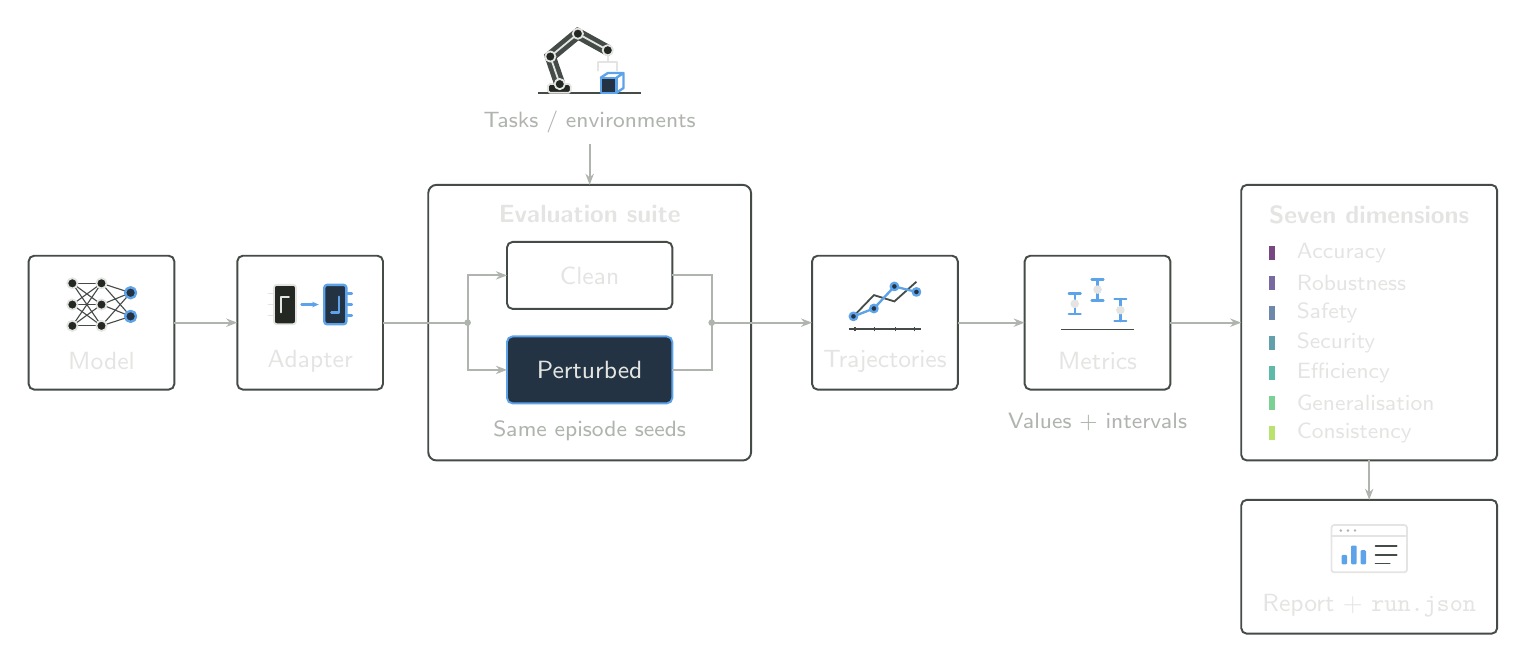
\begin{tikzpicture}[
  x=1cm,y=1cm,
  every node/.style={font=\sffamily\fontsize{9}{11}\selectfont,
    text=ink,inner sep=4pt,outer sep=0pt,align=center},
  box/.style={draw=rule,line width=0.7pt,rounded corners=2pt,
    minimum height=0.85cm,minimum width=1.85cm},
  note/.style={text=muted,font=\sffamily\fontsize{8}{10}\selectfont},
  flow/.style={draw=muted,line width=0.7pt,-{Stealth[length=4pt,width=3pt]}},
  wire/.style={draw=muted,line width=0.7pt},
  icon/.style={draw=ink,line width=0.65pt,line cap=round,line join=round},
  accenticon/.style={draw=signal,line width=0.85pt,line cap=round,line join=round},
  % Small vector illustrations share a two-tone palette and a 0.9 cm footprint.
  pics/model/.style={code={
    \foreach \a in {-0.27,0,0.27} {
      \foreach \b in {-0.27,0,0.27}
        \draw[draw=rule,line width=0.4pt] (-0.37,\a) -- (0,\b);
      \foreach \b in {-0.15,0.15}
        \draw[draw=rule,line width=0.4pt] (0,\a) -- (0.37,\b);
    }
    \foreach \x in {-0.37,0} {
      \foreach \y in {-0.27,0,0.27}
        \draw[icon,fill=panel] (\x,\y) circle (0.065);
    }
    \foreach \y in {-0.15,0.15}
      \draw[accenticon,fill=tint] (0.37,\y) circle (0.07);
  }},
  pics/adapter/.style={code={
    \draw[icon,fill=panel,rounded corners=1pt] (-0.46,-0.25) rectangle (-0.18,0.25);
    \draw[accenticon,fill=tint,rounded corners=1pt] (0.18,-0.25) rectangle (0.46,0.25);
    \foreach \y in {-0.14,0,0.14} {
      \draw[icon] (-0.53,\y) -- (-0.46,\y);
      \draw[accenticon] (0.46,\y) -- (0.53,\y);
    }
    \draw[accenticon,-{Stealth[length=2.4pt,width=2pt]}] (-0.11,0) -- (0.11,0);
    \draw[icon] (-0.37,-0.10) -- (-0.37,0.10) -- (-0.27,0.10);
    \draw[accenticon] (0.27,-0.10) -- (0.37,-0.10) -- (0.37,0.10);
  }},
  pics/trajectory/.style={code={
    \draw[draw=rule,line width=0.45pt] (-0.46,-0.31) -- (0.46,-0.31);
    \foreach \x in {-0.38,-0.13,0.13,0.38}
      \draw[draw=rule,line width=0.45pt] (\x,-0.34) -- (\x,-0.28);
    \draw[draw=rule,line width=0.65pt] (-0.40,-0.15) -- (-0.14,0.12) -- (0.12,0.04) -- (0.40,0.29);
    \draw[accenticon] (-0.40,-0.15) -- (-0.14,-0.05) -- (0.12,0.23) -- (0.40,0.16);
    \foreach \x/\y in {-0.40/-0.15,-0.14/-0.05,0.12/0.23,0.40/0.16}
      \draw[accenticon,fill=tint] (\x,\y) circle (0.047);
  }},
  pics/metrics/.style={code={
    \draw[draw=rule,line width=0.45pt] (-0.46,-0.32) -- (0.46,-0.32);
    \foreach \x/\y/\lo/\hi in {-0.29/0.01/-0.12/0.14,0/0.19/0.05/0.32,0.29/-0.07/-0.21/0.07} {
      \draw[accenticon] (\x,\lo) -- (\x,\hi)
        (\x-0.075,\lo) -- (\x+0.075,\lo)
        (\x-0.075,\hi) -- (\x+0.075,\hi);
      \fill[ink] (\x,\y) circle (0.055);
    }
  }},
  pics/scene/.style={code={
    % Articulated manipulator and an object on its work surface.
    \draw[draw=rule,line width=0.6pt] (-0.65,-0.38) -- (0.65,-0.38);
    \draw[icon,fill=panel,rounded corners=0.7pt] (-0.53,-0.38) rectangle (-0.24,-0.27);
    \draw[draw=rule,line width=4pt,line cap=round] (-0.38,-0.27) -- (-0.50,0.08) -- (-0.15,0.37) -- (0.23,0.16);
    \draw[icon] (-0.38,-0.27) -- (-0.50,0.08) -- (-0.15,0.37) -- (0.23,0.16);
    \foreach \x/\y in {-0.38/-0.27,-0.50/0.08,-0.15/0.37,0.23/0.16}
      \draw[icon,fill=panel] (\x,\y) circle (0.065);
    \draw[icon] (0.23,0.09) -- (0.23,0.01)
      (0.11,-0.10) -- (0.11,0.01) -- (0.35,0.01) -- (0.35,-0.10);
    \draw[accenticon,fill=tint] (0.14,-0.38) rectangle (0.34,-0.19);
    \draw[accenticon] (0.14,-0.19) -- (0.23,-0.13) -- (0.43,-0.13)
      -- (0.34,-0.19) (0.43,-0.13) -- (0.43,-0.32) -- (0.34,-0.38);
  }},
  pics/report/.style={code={
    \draw[icon,rounded corners=1pt] (-0.48,-0.30) rectangle (0.48,0.30);
    \draw[icon] (-0.48,0.16) -- (0.48,0.16);
    \foreach \x in {-0.36,-0.27,-0.18}
      \fill[muted] (\x,0.23) circle (0.018);
    \foreach \x/\h in {-0.35/0.12,-0.23/0.24,-0.11/0.18}
      \fill[signal,rounded corners=0.4pt] (\x,-0.20) rectangle ++(0.07,\h);
    \draw[draw=rule,line width=0.6pt,line cap=round]
      (0.08,0.03) -- (0.35,0.03) (0.08,-0.08) -- (0.35,-0.08)
      (0.08,-0.19) -- (0.26,-0.19);
  }},
]
% The suite branches into matched conditions, whose recorded trajectories feed
% the same metrics. Boxes denote operations or data, never illustrative scores.
\node[box,minimum height=1.70cm] (model) at (0,0) {};
\pic at (0,0.23) {model};
\node at (0,-0.49) {Model};
\node[box,minimum height=1.70cm] (adapter) at (2.65,0) {};
\pic at (2.65,0.23) {adapter};
\node at (2.65,-0.49) {Adapter};
\draw[flow] (model) -- (adapter);

\draw[draw=rule,line width=0.7pt,rounded corners=3pt]
  (4.15,-1.75) rectangle (8.25,1.75);
\node[font=\sffamily\bfseries\fontsize{9}{11}\selectfont]
  at (6.20,1.38) {Evaluation suite};
\node[box,minimum width=2.1cm] (clean) at (6.20,0.60) {Clean};
\node[box,minimum width=2.1cm,draw=signal,fill=tint]
  (perturbed) at (6.20,-0.60) {Perturbed};
\node[note] at (6.20,-1.38) {Same episode seeds};
\coordinate (split) at (4.65,0);
\draw[wire] (adapter.east) -- (split);
\draw[flow] (split) |- (clean.west);
\draw[flow] (split) |- (perturbed.west);
\fill[muted] (split) circle (1.2pt);

\pic at (6.20,3.30) {scene};
\node[note] (tasks) at (6.20,2.55) {Tasks / environments};
\draw[flow] (tasks.south) -- (6.20,1.75);

\node[box,minimum height=1.70cm] (trajectories) at (9.95,0) {};
\pic at (9.95,0.23) {trajectory};
\node at (9.95,-0.49) {Trajectories};
\coordinate (join) at (7.75,0);
\draw[wire] (clean.east) -| (join);
\draw[wire] (perturbed.east) -| (join);
\draw[flow] (join) -- (trajectories.west);
\fill[muted] (join) circle (1.2pt);
\node[box,minimum height=1.70cm] (metrics) at (12.65,0) {};
\pic at (12.65,0.23) {metrics};
\node at (12.65,-0.49) {Metrics};
\draw[flow] (trajectories) -- (metrics);
\node[note,anchor=north] at (12.65,-1.01) {Values + intervals};

% A compact, named output vector avoids fabricating a chart of model scores.
\node[box,minimum width=3.25cm,minimum height=3.50cm]
  (profile) at (16.10,0) {};
\node[font=\sffamily\bfseries\fontsize{9}{11}\selectfont]
  at (16.10,1.37) {Seven dimensions};
\foreach \y/\col/\title in {
  0.88/dimA/Accuracy,
  0.50/dimB/Robustness,
  0.12/dimC/Safety,
  -0.26/dimD/Security,
  -0.64/dimE/Efficiency,
  -1.02/dimF/Generalisation,
  -1.40/dimG/Consistency} {
  \fill[\col] (14.83,\y-0.09) rectangle ++(0.07,0.18);
  \node[anchor=west,font=\sffamily\fontsize{8.5}{10}\selectfont]
    at (15.04,\y) {\title};
}
\draw[flow] (metrics) -- (profile);
\node[box,minimum width=3.25cm,minimum height=1.70cm] (artifacts) at (16.10,-3.10) {};
\pic at (16.10,-2.87) {report};
\node at (16.10,-3.59) {Report + \texttt{run.json}};
\draw[flow] (profile) -- (artifacts);
\end{tikzpicture}
\end{document}
"
%   pdftocairo -svg method-light.pdf method-light.svg
%   pdftocairo -svg method-dark.pdf method-dark.svg
% Commit the SVGs; documentation builds do not require LaTeX.
\documentclass[border=8pt]{standalone}
\usepackage[T1]{fontenc}
\usepackage{lmodern}
\usepackage{xcolor}
\usepackage{tikz}
\usetikzlibrary{arrows.meta}
\providecommand{\xevalstheme}{light}
\def\xevalslight{light}
\ifx\xevalstheme\xevalslight
  \definecolor{ink}{HTML}{121412}
  \definecolor{muted}{HTML}{5C615D}
  \definecolor{rule}{HTML}{A8ADA7}
  \definecolor{panel}{HTML}{F1F2EF}
  \definecolor{signal}{HTML}{367FC9}
  \definecolor{tint}{HTML}{E8F0F8}
  \definecolor{dimA}{HTML}{440154}\definecolor{dimB}{HTML}{46327E}
  \definecolor{dimC}{HTML}{365C8D}\definecolor{dimD}{HTML}{277F8E}
  \definecolor{dimE}{HTML}{1FA187}\definecolor{dimF}{HTML}{4AC16D}
  \definecolor{dimG}{HTML}{A0DA39}
\else
  \definecolor{ink}{HTML}{E4E5E2}
  \definecolor{muted}{HTML}{AFB4AE}
  \definecolor{rule}{HTML}{454B46}
  \definecolor{panel}{HTML}{232823}
  \definecolor{signal}{HTML}{5DA3E9}
  \definecolor{tint}{HTML}{233344}
  \definecolor{dimA}{HTML}{774782}\definecolor{dimB}{HTML}{786AA0}
  \definecolor{dimC}{HTML}{6D88AB}\definecolor{dimD}{HTML}{62A1AC}
  \definecolor{dimE}{HTML}{5CBAA7}\definecolor{dimF}{HTML}{7BD194}
  \definecolor{dimG}{HTML}{B9E36E}
\fi
\begin{document}
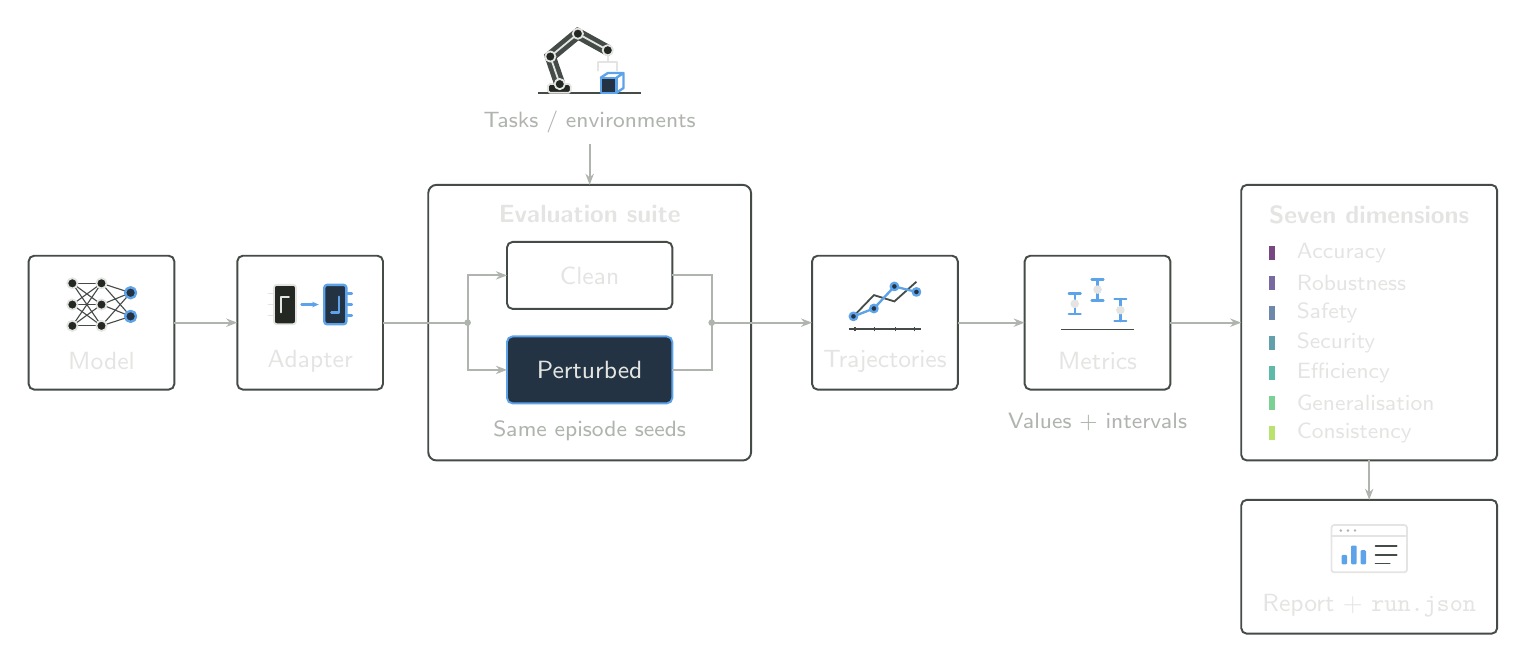
\begin{tikzpicture}[
  x=1cm,y=1cm,
  every node/.style={font=\sffamily\fontsize{9}{11}\selectfont,
    text=ink,inner sep=4pt,outer sep=0pt,align=center},
  box/.style={draw=rule,line width=0.7pt,rounded corners=2pt,
    minimum height=0.85cm,minimum width=1.85cm},
  note/.style={text=muted,font=\sffamily\fontsize{8}{10}\selectfont},
  flow/.style={draw=muted,line width=0.7pt,-{Stealth[length=4pt,width=3pt]}},
  wire/.style={draw=muted,line width=0.7pt},
  icon/.style={draw=ink,line width=0.65pt,line cap=round,line join=round},
  accenticon/.style={draw=signal,line width=0.85pt,line cap=round,line join=round},
  % Small vector illustrations share a two-tone palette and a 0.9 cm footprint.
  pics/model/.style={code={
    \foreach \a in {-0.27,0,0.27} {
      \foreach \b in {-0.27,0,0.27}
        \draw[draw=rule,line width=0.4pt] (-0.37,\a) -- (0,\b);
      \foreach \b in {-0.15,0.15}
        \draw[draw=rule,line width=0.4pt] (0,\a) -- (0.37,\b);
    }
    \foreach \x in {-0.37,0} {
      \foreach \y in {-0.27,0,0.27}
        \draw[icon,fill=panel] (\x,\y) circle (0.065);
    }
    \foreach \y in {-0.15,0.15}
      \draw[accenticon,fill=tint] (0.37,\y) circle (0.07);
  }},
  pics/adapter/.style={code={
    \draw[icon,fill=panel,rounded corners=1pt] (-0.46,-0.25) rectangle (-0.18,0.25);
    \draw[accenticon,fill=tint,rounded corners=1pt] (0.18,-0.25) rectangle (0.46,0.25);
    \foreach \y in {-0.14,0,0.14} {
      \draw[icon] (-0.53,\y) -- (-0.46,\y);
      \draw[accenticon] (0.46,\y) -- (0.53,\y);
    }
    \draw[accenticon,-{Stealth[length=2.4pt,width=2pt]}] (-0.11,0) -- (0.11,0);
    \draw[icon] (-0.37,-0.10) -- (-0.37,0.10) -- (-0.27,0.10);
    \draw[accenticon] (0.27,-0.10) -- (0.37,-0.10) -- (0.37,0.10);
  }},
  pics/trajectory/.style={code={
    \draw[draw=rule,line width=0.45pt] (-0.46,-0.31) -- (0.46,-0.31);
    \foreach \x in {-0.38,-0.13,0.13,0.38}
      \draw[draw=rule,line width=0.45pt] (\x,-0.34) -- (\x,-0.28);
    \draw[draw=rule,line width=0.65pt] (-0.40,-0.15) -- (-0.14,0.12) -- (0.12,0.04) -- (0.40,0.29);
    \draw[accenticon] (-0.40,-0.15) -- (-0.14,-0.05) -- (0.12,0.23) -- (0.40,0.16);
    \foreach \x/\y in {-0.40/-0.15,-0.14/-0.05,0.12/0.23,0.40/0.16}
      \draw[accenticon,fill=tint] (\x,\y) circle (0.047);
  }},
  pics/metrics/.style={code={
    \draw[draw=rule,line width=0.45pt] (-0.46,-0.32) -- (0.46,-0.32);
    \foreach \x/\y/\lo/\hi in {-0.29/0.01/-0.12/0.14,0/0.19/0.05/0.32,0.29/-0.07/-0.21/0.07} {
      \draw[accenticon] (\x,\lo) -- (\x,\hi)
        (\x-0.075,\lo) -- (\x+0.075,\lo)
        (\x-0.075,\hi) -- (\x+0.075,\hi);
      \fill[ink] (\x,\y) circle (0.055);
    }
  }},
  pics/scene/.style={code={
    % Articulated manipulator and an object on its work surface.
    \draw[draw=rule,line width=0.6pt] (-0.65,-0.38) -- (0.65,-0.38);
    \draw[icon,fill=panel,rounded corners=0.7pt] (-0.53,-0.38) rectangle (-0.24,-0.27);
    \draw[draw=rule,line width=4pt,line cap=round] (-0.38,-0.27) -- (-0.50,0.08) -- (-0.15,0.37) -- (0.23,0.16);
    \draw[icon] (-0.38,-0.27) -- (-0.50,0.08) -- (-0.15,0.37) -- (0.23,0.16);
    \foreach \x/\y in {-0.38/-0.27,-0.50/0.08,-0.15/0.37,0.23/0.16}
      \draw[icon,fill=panel] (\x,\y) circle (0.065);
    \draw[icon] (0.23,0.09) -- (0.23,0.01)
      (0.11,-0.10) -- (0.11,0.01) -- (0.35,0.01) -- (0.35,-0.10);
    \draw[accenticon,fill=tint] (0.14,-0.38) rectangle (0.34,-0.19);
    \draw[accenticon] (0.14,-0.19) -- (0.23,-0.13) -- (0.43,-0.13)
      -- (0.34,-0.19) (0.43,-0.13) -- (0.43,-0.32) -- (0.34,-0.38);
  }},
  pics/report/.style={code={
    \draw[icon,rounded corners=1pt] (-0.48,-0.30) rectangle (0.48,0.30);
    \draw[icon] (-0.48,0.16) -- (0.48,0.16);
    \foreach \x in {-0.36,-0.27,-0.18}
      \fill[muted] (\x,0.23) circle (0.018);
    \foreach \x/\h in {-0.35/0.12,-0.23/0.24,-0.11/0.18}
      \fill[signal,rounded corners=0.4pt] (\x,-0.20) rectangle ++(0.07,\h);
    \draw[draw=rule,line width=0.6pt,line cap=round]
      (0.08,0.03) -- (0.35,0.03) (0.08,-0.08) -- (0.35,-0.08)
      (0.08,-0.19) -- (0.26,-0.19);
  }},
]
% The suite branches into matched conditions, whose recorded trajectories feed
% the same metrics. Boxes denote operations or data, never illustrative scores.
\node[box,minimum height=1.70cm] (model) at (0,0) {};
\pic at (0,0.23) {model};
\node at (0,-0.49) {Model};
\node[box,minimum height=1.70cm] (adapter) at (2.65,0) {};
\pic at (2.65,0.23) {adapter};
\node at (2.65,-0.49) {Adapter};
\draw[flow] (model) -- (adapter);

\draw[draw=rule,line width=0.7pt,rounded corners=3pt]
  (4.15,-1.75) rectangle (8.25,1.75);
\node[font=\sffamily\bfseries\fontsize{9}{11}\selectfont]
  at (6.20,1.38) {Evaluation suite};
\node[box,minimum width=2.1cm] (clean) at (6.20,0.60) {Clean};
\node[box,minimum width=2.1cm,draw=signal,fill=tint]
  (perturbed) at (6.20,-0.60) {Perturbed};
\node[note] at (6.20,-1.38) {Same episode seeds};
\coordinate (split) at (4.65,0);
\draw[wire] (adapter.east) -- (split);
\draw[flow] (split) |- (clean.west);
\draw[flow] (split) |- (perturbed.west);
\fill[muted] (split) circle (1.2pt);

\pic at (6.20,3.30) {scene};
\node[note] (tasks) at (6.20,2.55) {Tasks / environments};
\draw[flow] (tasks.south) -- (6.20,1.75);

\node[box,minimum height=1.70cm] (trajectories) at (9.95,0) {};
\pic at (9.95,0.23) {trajectory};
\node at (9.95,-0.49) {Trajectories};
\coordinate (join) at (7.75,0);
\draw[wire] (clean.east) -| (join);
\draw[wire] (perturbed.east) -| (join);
\draw[flow] (join) -- (trajectories.west);
\fill[muted] (join) circle (1.2pt);
\node[box,minimum height=1.70cm] (metrics) at (12.65,0) {};
\pic at (12.65,0.23) {metrics};
\node at (12.65,-0.49) {Metrics};
\draw[flow] (trajectories) -- (metrics);
\node[note,anchor=north] at (12.65,-1.01) {Values + intervals};

% A compact, named output vector avoids fabricating a chart of model scores.
\node[box,minimum width=3.25cm,minimum height=3.50cm]
  (profile) at (16.10,0) {};
\node[font=\sffamily\bfseries\fontsize{9}{11}\selectfont]
  at (16.10,1.37) {Seven dimensions};
\foreach \y/\col/\title in {
  0.88/dimA/Accuracy,
  0.50/dimB/Robustness,
  0.12/dimC/Safety,
  -0.26/dimD/Security,
  -0.64/dimE/Efficiency,
  -1.02/dimF/Generalisation,
  -1.40/dimG/Consistency} {
  \fill[\col] (14.83,\y-0.09) rectangle ++(0.07,0.18);
  \node[anchor=west,font=\sffamily\fontsize{8.5}{10}\selectfont]
    at (15.04,\y) {\title};
}
\draw[flow] (metrics) -- (profile);
\node[box,minimum width=3.25cm,minimum height=1.70cm] (artifacts) at (16.10,-3.10) {};
\pic at (16.10,-2.87) {report};
\node at (16.10,-3.59) {Report + \texttt{run.json}};
\draw[flow] (profile) -- (artifacts);
\end{tikzpicture}
\end{document}
